% LaTeX source for ``Think Stats:
% Probability and Statistics for Programmers''
% Copyright 2014  Allen B. Downey.

% License: Creative Commons Attribution-NonCommercial 3.0 Unported License.
% http://creativecommons.org/licenses/by-nc/3.0/
%

%\documentclass[10pt,b5paper]{book}
\documentclass[12pt]{book}
\usepackage[width=5.5in,height=8.5in,
  hmarginratio=3:2,vmarginratio=1:1]{geometry}

% for some of these packages, you might have to install
% texlive-latex-extra (in Ubuntu)

\usepackage[T1]{fontenc}
\usepackage{textcomp}
\usepackage{mathpazo}

%\usepackage{pslatex}

\usepackage{url}
\usepackage{fancyhdr}
\usepackage{graphicx}
\usepackage{subfig}
\usepackage{amsmath}
\usepackage{amsthm}
%\usepackage{amssymb}
\usepackage{makeidx}
\usepackage{setspace}
\usepackage{hevea}                           
\usepackage{upquote}

\title{Think Stats}
\author{Allen B. Downey}

\newcommand{\thetitle}{Think Stats: Probability and Statistics for Programmers}
\newcommand{\theversion}{2.0.1}

% these styles get translated in CSS for the HTML version
\newstyle{a:link}{color:black;}
\newstyle{p+p}{margin-top:1em;margin-bottom:1em}
\newstyle{img}{border:0px}

% change the arrows in the HTML version
\setlinkstext
  {\imgsrc[ALT="Previous"]{back.png}}
  {\imgsrc[ALT="Up"]{up.png}}
  {\imgsrc[ALT="Next"]{next.png}} 

\makeindex

\newif\ifplastex
\plastexfalse

\begin{document}

\frontmatter

\newcommand{\Erdos}{Erd\H{o}s}
\newcommand{\nhat}{\hat{N}}
\newcommand{\eps}{\varepsilon}
\newcommand{\slope}{\beta}
\newcommand{\inter}{\alpha}
\newcommand{\xbar}{\bar{x}}
\newcommand{\ybar}{\bar{y}}
\newcommand{\PMF}{\mathrm{PMF}}
\newcommand{\PDF}{\mathrm{PDF}}
\newcommand{\CDF}{\mathrm{CDF}}
\newcommand{\ICDF}{\mathrm{ICDF}}
\newcommand{\Prob}{\mathrm{P}}
\newcommand{\Corr}{\mathrm{Corr}}
\newcommand{\normal}{\mathcal{N}}
\newcommand{\given}{|}
\newcommand{\goodchi}{\protect\raisebox{2pt}{$\chi$}}

\ifplastex
    \usepackage{localdef}
    \maketitle

\newcount\anchorcnt
\newcommand*{\Anchor}[1]{%
  \@bsphack%
    \Hy@GlobalStepCount\anchorcnt%
    \edef\@currentHref{anchor.\the\anchorcnt}% 
    \Hy@raisedlink{\hyper@anchorstart{\@currentHref}\hyper@anchorend}% 
    \M@gettitle{}\label{#1}% 
    \@esphack%
}


\else

%%% EXERCISE

\newtheoremstyle{exercise}% name of the style to be used
  {\topsep}% measure of space to leave above the theorem. E.g.: 3pt
  {\topsep}% measure of space to leave below the theorem. E.g.: 3pt
  {}% name of font to use in the body of the theorem
  {0pt}% measure of space to indent
  {\bfseries}% name of head font
  {}% punctuation between head and body
  { }% space after theorem head; " " = normal interword space
  {}% Manually specify head

\theoremstyle{exercise}
\newtheorem{exercise}{Exercise}[chapter]

%\newcounter{exercise}[chapter]
%\newcommand{\nextexercise}{\refstepcounter{exercise}}

%\newenvironment{exercise}{\nextexercise \noindent \textbf{Exercise \thechapter.\theexercise} \begin{itshape} \noindent}{\end{itshape}}

\input{latexonly}

\begin{latexonly}

\renewcommand{\blankpage}{\thispagestyle{empty} \quad \newpage}

%\blankpage
%\blankpage

% TITLE PAGES FOR LATEX VERSION

%-half title--------------------------------------------------
\thispagestyle{empty}

\begin{flushright}
\vspace*{2.0in}

\begin{spacing}{3}
{\huge Think Stats: Probability and Statistics for Programmers}\\
{\Large }
\end{spacing}

\vspace{0.25in}

Version \theversion

\vfill

\end{flushright}

%--verso------------------------------------------------------

\blankpage
\blankpage
%\clearemptydoublepage
%\pagebreak
%\thispagestyle{empty}
%\vspace*{6in}

%--title page--------------------------------------------------
\pagebreak
\thispagestyle{empty}

\begin{flushright}
\vspace*{2.0in}

\begin{spacing}{3}
{\huge Think Stats}\\
{\Large Probability and Statistics for Programmers}
\end{spacing}

\vspace{0.25in}

Version \theversion

\vspace{1in}


{\Large
Allen B. Downey\\
}


\vspace{0.5in}

{\Large Green Tea Press}

{\small Needham, Massachusetts}

%\includegraphics[width=1in]{figs/logo1.eps}
\vfill

\end{flushright}


%--copyright--------------------------------------------------
\pagebreak
\thispagestyle{empty}

{\small
Copyright \copyright ~2014 Allen B. Downey.


\vspace{0.2in}

\begin{flushleft}
Green Tea Press       \\
9 Washburn Ave \\
Needham MA 02492
\end{flushleft}

Permission is granted to copy, distribute, and/or modify this document
under the terms of the Creative Commons Attribution-NonCommercial 3.0 Unported
License, which is available at \url{http://creativecommons.org/licenses/by-nc/3.0/}.

The original form of this book is \LaTeX\ source code.  Compiling this
code has the effect of generating a device-independent representation
of a textbook, which can be converted to other formats and printed.

The \LaTeX\ source for this book is available from
\url{http://thinkstats2.com}.

The cover for this book is based on a photo by Paul Friel
(\url{http://flickr.com/people/frielp/}), who made it available under
the Creative Commons Attribution license.  The original photo
is at \url{http://flickr.com/photos/frielp/11999738/}.

\vspace{0.2in}

} % end small

\end{latexonly}


% HTMLONLY

\begin{htmlonly}

% TITLE PAGE FOR HTML VERSION

{\Large \thetitle}

{\large Allen B. Downey}

Version \theversion

\vspace{0.25in}

Copyright 2014 Allen B. Downey

\vspace{0.25in}

Permission is granted to copy, distribute, and/or modify this document
under the terms of the Creative Commons Attribution-NonCommercial 3.0
Unported License, which is available at
\url{http://creativecommons.org/licenses/by-nc/3.0/}.

\setcounter{chapter}{-1}

\end{htmlonly}

\fi
% END OF THE PART WE SKIP FOR PLASTEX

\chapter{Preface}
\label{preface}

\section*{Why I wrote this book}

{\em Think Stats: Probability and Statistics for Programmers} is an
introduction to the practical tools of exploratory data analysis.

When I start working with a new dataset, I follow these steps:

\begin{itemize}

\item Importing and cleaning: Whatever format the data is in, it
usually takes some time and effort to read the data, clean and transform
it, and check that everything made it through the translation process
intact.

\item Single variable explorations: I usually start by examining one
  variable at a time, finding out what the values mean and what
  distributions of the variables are, and identifying appropriate
  summary statistics.

\item Pair-wise explorations: To identify possible relationships
  between variables, I look at tables and scatter plots, and compute
  correlations and linear fits.

\item Multivariate analysis: If there are apparent relationships
  between variables, I use multiple regression to add control variables
  investigate more complex relationships.

\item Estimation and hypothesis testing: When reporting statistical
  results, it is important to answer three questions: How big is
  the effect?  How much variability should we expect if we run the same
  measurement again?  Is it likely that the apparent effect could be
  due to chance?

\item Visualization: During exploration, visualization is an important 
  tool for finding possible relationships and effects.  Then if an
  apparent effect holds up to scrutiny, visualization is an effective
  way to communicate results.

\end{itemize}


This books takes a computational approach, which has several
advantages:

\begin{itemize}

\item I present most ideas using simple Python code, rather than
  mathematical notation.  In general, Python code is more readble;
  also, because it is executable, readers can download it, run it,
  and modify it.

\item Each chapter includes exercies readers can do to develop
  and solidify their learning.  When you write programs, you
  express your understanding in code; when you debugging the
  program, you are correcting your understanding.

\item Some exercises involve running experiments to test statistical
  behavior.  For example, you can explore the Central Limit Theorem
  (CLT) by generating random samples and computing their sums.  The
  resulting visualizations demonstrate why the CLT works, and when
  it doesn't.

\item Some ideas that are hard to grasp mathematically are easy to
  understand by simulation.  For example, we approximate p-values by
  running Monte Carlo simulations, which reinforces the meaning of the
  p-value.

\item Because the book is based on a general-purpose programming language
  (Python), readers can import data from almost any
  source.  They are not limited to data that has been cleaned and
  formatted for a particular statistics tool.

\end{itemize}

The book lends itself to a project-based approach.  In my class,
students work on a semester-long project that requires them to pose a
statistical question, find a dataset that can address it, and apply
each of the techniques they learn to their own data.

To demonstrate my approach to exploratory data analysis, the book
presents a case study that runs through all of the chapters.  It uses
data from two sources:

\begin{itemize}

\item The National Survey of Family Growth (NSFG), conducted by the
  U.S. Centers for Disease Control and Prevention (CDC) to gather
  ``information on family life, marriage and divorce, pregnancy,
  infertility, use of contraception, and men's and women's health.''
  (See \url{http://cdc.gov/nchs/nsfg.htm}.)

\item The Behavioral Risk Factor Surveillance System (BRFSS),
  conducted by the National Center for Chronic Disease Prevention and
  Health Promotion to ``track health conditions and risk behaviors in
  the United States.''  (See \url{http://cdc.gov/BRFSS/}.)

\end{itemize}

Other examples use data from the IRS, the U.S. Census, and
the Boston Marathon.


\section*{How I wrote this book}

When people write a new textbook, they usually start by
reading a stack of old textbooks.  As a result, most books
contain the same material in pretty much the same order.  Often there
are phrases, and errors, that propagate from one book to the next;
Stephen Jay Gould pointed out an example in his essay, ``The Case of
the Creeping Fox Terrier.''\footnote{A breed of dog that is about half
  the size of a Hyracotherium (see
  \url{http://wikipedia.org/wiki/Hyracotherium}).}

I did not do that.  In fact, I used almost no printed material while I
was writing this book, for several reasons:

\begin{itemize}

\item My goal was to explore a new approach to this material, so I didn't
want much exposure to existing approaches.

\item Since I am making this book available under a free license, I wanted
to make sure that no part of it was encumbered by copyright restrictions.

\item Many readers of my books don't have access to libraries of
printed material, so I tried to make references to resources that are
freely available on the Internet.

\item Some proponents of old media think that the exclusive
use of electronic resources is lazy and unreliable.  They might be right
about the first part, but I think they are wrong about the second, so
I wanted to test my theory.

% http://www.ala.org/ala/mgrps/rts/nmrt/news/footnotes/may2010/in_defense_of_wikipedia_bonnett.cfm

\end{itemize}

The resource I used more than any other is Wikipedia, the bugbear
of librarians everywhere.  In general, the articles I read on
statistical topics were very good (although I made a few small changes
along the way).  I include references to Wikipedia pages throughout
the book and I encourage you to follow those links; in many cases, the
Wikipedia page picks up where my description leaves off.  The
vocabulary and notation in this book are generally consistent with
Wikipedia, unless I had a good reason to deviate.
Other resources I found useful were Wolfram MathWorld and (of course)
Google.

\section*{Using the code}

The code and data used in this book are available from
\url{https://github.com/AllenDowney/ThinkStats2}.  Git is a version
control system that allows you to keep track of the files that
make up a project.  A collection of files under Git's control is
called a {\bf repository}.  GitHub is a hosting service that provides
storage for Git repositories and a convenient web interface.

The GitHub homepage for my repostory provides several ways to
work with the code:

\begin{itemize}

\item You can create a copy of my repository
on GitHub by pressing the {\sf Fork} button.  If you don't already
have a GitHub account, you'll need to create one, but if you do, you'll
have your own repository on GitHub that you can use to keep track
of code you write while working on this book.

\item You can also {\bf clone}
my repository, which means that you create a copy of the files on
your computer.  You don't need a GitHub account to do this, but you
won't be able to write your changes back to my repository.

\item If you don't want to use Git at all, you can download the files
in a Zip file.

\end{itemize}

The code in this book is written to work in both Python 2 and Python 3
with no translation.  However, you will need the following packages
installed: 

\begin{itemize}

\item pandas for representing and analyzing data,
  \url{http://pandas.pydata.org/}.

\item NumPy for basic numerical computation, \url{http://www.numpy.org/}.

\item SciPy for scientific computation including statistics,
  \url{http://www.scipy.org/}.

\item matplotlib for visualization, \url{http://matplotlib.org/}.

\end{itemize}

Although these are commonly-used packages, they are not included with
all Python installations, and they can be hard to install in some
environments.  I developed this book using Anaconda from Continuum
Analytics, which is a free Python distribution that includes all
packages you'll need to run the code (and lots more).

I found Anaconda easy to install.  By default it does a user-level
installation, not system-level, so you don't need administrative
privilege.  And it supports both Python 2 and Python 3.  You can
download Anaconda from \url{http://continuum.io/downloads}.

After you clone the repository or unzip the zip file, you should
have a file called {\tt ThinkStats2/code/nsfg.py}.  If you run it,
it should read a data file, run some tests, and print a message
like, ``All tests passed.''  If you get import errors, it probably
means there are some packages you need to install.  Good luck!


Allen B. Downey \\*
Needham MA \\*

Allen B. Downey is a Professor of Computer Science at 
the Franklin W. Olin College of Engineering.




%\section*{Acknowledgements}



\section*{Contributor List}

If you have a suggestion or correction, please send email to 
{\tt downey@allendowney.com}.  If I make a change based on your
feedback, I will add you to the contributor list
(unless you ask to be omitted).
\index{contributors}

If you include at least part of the sentence the
error appears in, that makes it easy for me to search.  Page and
section numbers are fine, too, but not quite as easy to work with.
Thanks!

\small

\begin{itemize}

\item Lisa Downey and June Downey read an early draft and made many
corrections and suggestions.

\item Steven Zhang found several errors.

\item Andy Pethan and Molly Farison helped debug some of the solutions,
and Molly spotted several typos.

\item Andrew Heine found an error in my error function.

\item Dr. Nikolas Akerblom knows how big a Hyracotherium is.

\item Alex Morrow clarified one of the code examples.

\item Jonathan Street caught an error in the nick of time.

\item G\'{a}bor Lipt\'{a}k found a typo in the book and the relay race solution.

\item Many thanks to Kevin Smith and Tim Arnold for their work on
plasTeX, which I used to convert this book to DocBook.

\item George Caplan sent several suggestions for improving clarity.

\item Julian Ceipek found an error and a number of typos.

\item Stijn Debrouwere, Leo Marihart III, Jonathan Hammler, and Kent Johnson
found errors in the first print edition.

\item Dan Kearney found a typo.

\item Jeff Pickhardt found a broken link and a typo.

\item J\"{o}rg Beyer found typos in the book and made many corrections
in the docstrings of the accompanying code.

\item Tommie Gannert sent a patch file with a number of corrections.

\item Alexander Gryzlov suggested a clarification in an exercise.

\item Martin Veillette reported an error in one of the formulas for
Pearson's correlation.

\item Christoph Lendenmann submitted several errata.

\item Haitao Ma noticed a typo and and sent me a note.

% ENDCONTRIB

\end{itemize}

\normalsize

\clearemptydoublepage

% TABLE OF CONTENTS
\begin{latexonly}

\tableofcontents

\clearemptydoublepage

\end{latexonly}

% START THE BOOK
\mainmatter


\chapter{Data science for programmers}
\label{intro}

The thesis of this book is that data, combined with practical
methods, can answer questions and guide decisions under uncertainty.

As an example, I present a case study motivated by a question
I heard when my wife and I were expecting our first child: do first
babies tend to arrive late?
\index{first babies}

If you Google this question, you will find plenty of
discussion.  Some people claim
it's true, others say it's a myth, and some people say it's the other
way around: first babies come early.

In many of these discussions, people provide data to support their
claims.  I found many examples like these:

\begin{quote}

``My two friends that have given birth recently to their first babies,
BOTH went almost 2 weeks overdue before going into labour or being
induced.''

``My first one came 2 weeks late and now I think the second one is
going to come out two weeks early!!''

``I don't think that can be true because my sister was my mother's
first and she was early, as with many of my cousins.''

\end{quote}

Reports like these are called {\bf anecdotal evidence} because they
are based on data that is unpublished and usually personal.  In casual
conversation, there is nothing wrong with anecdotes, so I don't mean
to pick on the people I quoted.
\index{anecdotal evidence}

But we might want evidence that is more persuasive and
an answer that is more reliable.  By those standards, anecdotal
evidence usually fails, because:

\begin{itemize}

\item Small number of observations: If the gestation period is longer
  for first babies, the difference is probably small compared to
  natural variation.  In that case, we might have to compare a large
  number of pregnancies to be sure that a difference exists.
\index{sample size}

\item Selection bias: People who join a discussion of this question
  might be interested because their first babies were late.  In that
  case the process of selecting data would bias the results.
\index{selection bias}
\index{bias!selection}

\item Confirmation bias:  People who believe the claim might be more
  likely to contribute examples that confirm it.  People who doubt the
  claim are more likely to cite counterexamples.
\index{confirmation bias}
\index{bias!confirmation}

\item Inaccuracy: Anecdotes are often personal stories, and often
  misremembered, misrepresented, repeated
  inaccurately, etc.

\end{itemize}

So how can we do better?

\section{A statistical approach}

To address the limitations of anecdotes, we will use the tools
of statistics, which include:

\begin{itemize}

\item Data collection: We will use data from a large national survey
  that was designed explicitly with the goal of generating
  statistically valid inferences about the U.S. population.
\index{data collection}

\item Descriptive statistics: We will generate statistics that
  summarize the data concisely, and evaluate different ways to
  visualize data.
\index{descriptive statistics}

\item Exploratory data analysis: We will look for
  patterns, differences, and other features that address the questions
  we are interested in.  At the same time we will check for
  inconsistencies and identify limitations.
\index{exploratory data analysis}

\item Estimation: We will use data from a sample to estimate
  characteristics of the general population.
\index{estimation}

\item Hypothesis testing: Where we see apparent effects, like a
  difference between two groups, we will evaluate whether the effect
  might have happened by chance.
\index{hypothesis testing}

\end{itemize}

By performing these steps with care to avoid pitfalls, we can
reach conclusions that are more justifiable and more likely to be
correct.


\section{The National Survey of Family Growth}
\label{nsfg}

Since 1973 the U.S. Centers for Disease Control and Prevention (CDC)
have conducted the National Survey of Family Growth (NSFG),
which is intended to gather ``information on family life, marriage and
divorce, pregnancy, infertility, use of contraception, and men's and
women's health. The survey results are used ... to plan health services and
health education programs, and to do statistical studies of families,
fertility, and health.''\footnote{See
  \url{http://cdc.gov/nchs/nsfg.htm}.}
\index{National Survey of Family Growth}
\index{NSFG}

We will use data collected by this survey to investigate whether first
babies tend to come late, and other questions.  In order to use this
data effectively, we have to understand the design of the study.

The NSFG is a {\bf cross-sectional} study, which means that it
captures a snapshot of a group at a point in time.  The most
common alternative is a {\bf longitudinal} study, which observes a
group repeatedly over a period of time.
\index{cross-sectional study}
\index{study!cross-sectional}
\index{longitudinal study}
\index{study!longitudinal}

The NSFG has been conducted seven times; each deployment is called
a {\bf cycle}.  We will use data from Cycle 6, which was
conducted from January 2002 to March 2003.
\index{cycle}

The goal of the survey is to draw conclusions about a
{\bf population}; the target population of the NSFG is people in
the United States aged 15-44.
\index{population}

The people who participate in a survey are called {\bf respondents};
a group of respondents is called a {\bf cohort}.
In general, cross-sectional studies are meant to be {\bf
  representative}, which means that every member of the target
population has an equal chance of participating.  Of course that ideal
is hard to achieve in practice, but people who conduct surveys come as
close as they can.
\index{respondent}
\index{representative}

The NSFG is not representative; instead it is deliberately {\bf
  oversampled}.  The designers of the study recruited three
groups---Hispanics, African-Americans and teenagers---at rates higher
than their representation in the U.S. population.
The reason for oversampling is to make sure that the number of
respondents in each of these groups is large enough to draw valid
statistical inferences.
\index{oversampling}

Of course, the drawback of oversampling is that it is not as easy
to draw conclusions about the general population based on statistics
from the survey.  We will come back to this point later.

\begin{exercise}

Although the NSFG has been conducted seven times, it is not a
longitudinal study.  Read the Wikipedia pages
\url{http://wikipedia.org/wiki/Cross-sectional_study}
and
\url{http://wikipedia.org/wiki/Longitudinal_study}
to make sure you understand why not.

\end{exercise}


\section{Importing the data}

The code and data used in this book are available from
\url{https://github.com/AllenDowney/ThinkStats2}.  For information
about downloading and working with this code, see Section~\ref{code}.

Once you download the code, you should
have a file called {\tt ThinkStats2/code/nsfg.py}.  If you run it,
it should read a data file, run some tests, and print a message
like, ``All tests passed.''

Let's see what it does.  Pregnancy data from Cycle 6 of the NSFG is in
a file called {\tt 2002FemPreg.dat.gz}.  As the suffixes suggest, it
is a gzip-compressed data file in plain text (ASCII), with fixed width
columns.  Each line in the file contains data about one pregnancy.

The format of the file is documented in {\tt 2002FemPreg.dct}, which
is a Stata dictionary file.  Stata is a statistical software system;
a ``dictionary'' in this context is a list of variable names and types,
and indices that indicate where in each line to find each variable.

For example:
%
\begin{verbatim}
infile dictionary {
  _column(1)  str12  caseid    %12s  "RESPONDENT ID NUMBER"
  _column(13) byte   pregordr   %2f  "PREGNANCY ORDER (NUMBER)"
}
\end{verbatim}

This dictionary describes two variables: {\tt caseid} is a 12-character
string that represents the respondent ID; {\tt pregorder} is a 
one-byte integer that indicates which pregnancy this record
describes for this respondent.

The code you downloaded includes {\tt ThinkStats2} which is a library
that contains many classes and functions used in this book.  {\tt
  ThinkStats2} provides functions to read the Stata dictionary and
then use it to read the NSFG data file.

Here's how it's used in {\tt nsfg.py}:

\begin{verbatim}
def ReadFemPreg(dct_file = '2002FemPreg.dct',
                dat_file = '2002FemPreg.dat.gz'):
    dct = thinkstats2.ReadStataDct(dct_file)
    df = dct.ReadFixedWidth(dat_file, compression='gzip')
    CleanPregFrame(df)
    return df
\end{verbatim}

{\tt thinkstats2.ReadStataDct} takes the name of the dictionary file
and returns a FixedWidthVariables object, which contains the information
from the dictionary file and provides {\tt ReadFixedWidth}, which
reads the data file.

The result is a DataFrame, which is the fundamental data structure
provided by Pandas.  A DataFrame behaves like a list in some ways,
like an array in other ways, and also like a dictionary.

You can think of it as an array that contains a row for
each record, in this case one row per pregnancy, and a column for
each variable.

In addition to the data, a DataFrame also contains the variable
names and their types, and it provides methods for accessing and modifying
the data.


\section{Variables}

For pregnancy records, we extract the following variables:

\begin{itemize}

\item caseid] is the integer ID of the respondent.

\item prglength] is the integer duration of the pregnancy in weeks.

\item outcome] is an integer code for the outcome of the pregnancy.
The code 1 indicates a live birth.

\item birthord] is the integer birth order of each live birth;
for example, the code for a first child is 1. 
For outcomes other than live birth, this field is blank.

\item finalwgt] is the statistical weight associated with the respondent.
It is a floating-point value that indicates the number of people in
the U.S. population this respondent represents.  Members of oversampled
groups have lower weights.\index{weight!sample}

\end{itemize}

If you read the casebook carefully, you will see that most of these
variables are {\bf recodes}, which means that they are not part of the
{\bf raw data} collected by the survey, but they are calculated using
the raw data.  \index{recode} \index{raw data}

For example, {\tt prglength} for live births is equal to the raw
variable {\tt wksgest} (weeks of gestation) if it is available;
otherwise it is estimated using {\tt mosgest * 4.33} (months of
gestation times the average number of weeks in a month).

Recodes are often based on logic that checks the consistency and
accuracy of the data.  In general it is a good idea to use recodes
unless there is a compelling reason to process the raw data
yourself.

You might also notice that {\tt Pregnancies} has a method called
{\tt Recode} that does some additional checking and recoding.




\section{DataFrames}

For now you can think of a DataFrame as a dictionary that maps from
each column name to a column of data.  The attribute {\tt columns}
is a list of column names:  

\begin{verbatim}
>>> import nsfg
>>> df = ReadFemPreg()
>>> df.columns
Index([u'caseid', u'pregordr', u'howpreg_n', u'howpreg_p', ... ])
\end{verbatim}

The result is an Index, which is another Pandas data structure.  For
now, we'll treat it like a list:

\begin{verbatim}
>>> df.columns[1]
'pregordr'
\end{verbatim}

To access a column from a DataFrame, you can use the variable
name as a key:

\begin{verbatim}
>>> pregordr = df['pregordr']
>>> type(pregordr)
<class 'pandas.core.series.Series'>
\end{verbatim}

The result is a Series, yet another Pandas data structure.
For now, you can think of a Series as a list, but there's
a bit more to it.  When you print a Series, you get the indices and the
corresponding values:

\begin{verbatim}
>>> pregordr
0     1
1     2
2     1
3     2
...
13590    3
13591    4
13592    5
Name: pregordr, Length: 13593, dtype: int64
\end{verbatim}

In addition, the Series prints the variable name, length, and data type;
{\tt int64} is one of the types provided by NumPy.  If you run
this example on a 32-bit machine you might see {\tt int32}.

You can access the elements of a Series using integer indices
and slices:

\begin{verbatim}
>>> pregordr[0]
1
>>> pregordr[2:5]
2    1
3    2
4    3
Name: pregordr, dtype: int64
\end{verbatim}

The result of the index operator is an {\tt int64}; the
result of the slice is another Series.

You can also access the columns of a DataFrame using dot notation:

\begin{verbatim}
>>> pregordr = df.pregordr
\end{verbatim}

This notation only works if the column name is a valid Python
identifier, so it has to begin with a letter, can't contain spaces, etc.


\section{Transformation}

When you import data like this, you often have to check for errors,
deal with special values, convert data into different formats, and
perform calculations.  These operations are called {\bf data cleaning}.

{\tt nsfg.py} includes {\tt CleanPregFrame}, a function that cleans
the variables I am planning to use.

\begin{verbatim}
def CleanPregFrame(df):
    df.agepreg /= 100.0

    na_vals = [97, 98, 99]
    df.birthwgt_lb.replace(na_vals, np.nan, inplace=True)
    df.birthwgt_oz.replace(na_vals, np.nan, inplace=True)

    df.totalwgt_lb = df.birthwgt_lb + df.birthwgt_oz / 16.0    
\end{verbatim}

{\tt agepreg} contains the mother's age at the end of the
pregnancy.  
In the data file, {\tt agepreg} is encoded as an integer
number of centiyears.  So the first line divides each element
of {\tt agepreg} by 100, yielding a floating-point value in
years.

\verb"birthwgt_lb" and \verb"birthwgt_oz" contain the weight of the
baby, in pounds and ounces, for pregnancies that end in live birth.
In addition it uses several special codes:

\begin{verbatim}
97	NOT ASCERTAINED
98	REFUSED	 
99	DON'T KNOW
\end{verbatim}

Special values that are encoded as numbers are {\em dangerous} because
if they are not handled properly, they can easily introduce bogus
values.  The {\tt replace} method replaces these values with {\tt NaN}, 
a special floating-point value that represents 
``not a number.''  {\tt nan} is available from NumPy, which I imported
as {\tt np}.

As part of the IEEE floating-point standard, all mathematical
operations return {\tt nan} if either argument is {\tt nan}:

\begin{verbatim}
>>> import numpy as np
>>> np.nan / 100.0
\end{verbatim}

So computations with {\tt nan} tend to do the right thing.  And
most Pandas functions handle {\tt nan} appropriately, at
least for most applications.  But this will be a recurring issue.

Finally, the last line of {\tt CleanPregFrame} creates a new
column \verb"totalwgt_lb" that combines pounds and ounces into
a single quantity, in pounds.



\section{Validation}


In my initial exploration of this dataset, I found one value in
\verb"birthwgt_lb" that is clearly wrong, unless one of the babies
in this dataset was actually 51 pounds at birth.  So I added
this line to replace invalid values with {\tt NaN}:

\begin{verbatim}
df.birthwgt_lb[df.birthwgt_lb > 20] = np.nan
\end{verbatim}

The expression in brackets yields a Series of type {\tt bool}, 
where True indicates that the condition is true.  When a boolean
Series is used as an index, it selects only the elements that
satisfy the condition; in this case, it replaces them with {\tt NaN}.

\begin{verbatim}
\end{verbatim}

\begin{verbatim}
\end{verbatim}

\begin{verbatim}
\end{verbatim}



\section{Interpretation}

To work with data effectively, you have to think on two levels at the
same time: the level of statistics and the level of context.

As an example, let's look at the sequence of outcomes for a few
respondents.  Because of the way the data files are organized, we have
to do some processing to match up each pregnancy record with a respondent.
Here's a function that does that:

\begin{verbatim}
def MakePregMap(df):
    d = {}
    for index, caseid in df.caseid.iteritems():
        d.setdefault(caseid, []).append(index)
    return d
\end{verbatim}

{\tt df} is the DataFrame with pregnancy data.  The {\tt iteritems}
method creates an iterator that enumerates the index (row number)
and {\tt caseid} for each pregnancy.

{\tt d} is a dictionary that maps from each caseid to a list of
indices, so for each respondent we can look up the indices of
that respondent's pregnancies.

This example looks up one respondent and prints a list of outcomes
for her pregnancies:

\begin{verbatim}
    caseid = 10229
    indices = preg_map[caseid]
    print(caseid, preg.outcome[indices].values)
\end{verbatim}

And here is the result:

\begin{verbatim}
10229 [4 4 4 4 4 4 1]
\end{verbatim}

The outcome code {\tt 1} indicates a live birth. Code {\tt 4} indicates
a miscarriage; that is, a preganancy that ended spontaneously, usually
with no known medical cause.

Statistically this respondent is not unusual.  Miscarriages are common
and there are other respondents who reported as many or more.

But remembering the context, this data tells the story of a woman
who was pregnant six times, each time ending in miscarriage.  If we
look at this data with empathy, it is natural to infer from her
persistence how much she wanted a child, and to feel some joy at
the successful outcome of her seventh pregnancy.

Each record in the NSFG dataset represents a person who provided
honest answers to many personal and difficult questions.  We can use
this data to answer statistical questions about family life,
reproduction, and health.  At the same time, we should remember the
context, and the people, the data come from.



\section{Exercises}



\begin{exercise}
In this exercise you will write a program to explore the data
in the Pregnancies table.


\end{exercise}


\begin{exercise}
The best way to learn about statistics is to work on a project you are
interested in.  Is there a question like, ``Do first babies arrive
late,'' that you would like to investigate?

Think about questions you find personally interesting, or items of
conventional wisdom, or controversial topics, or questions that have
political consequences, and see if you can formulate a question that
lends itself to statistical inquiry.

Look for data to help you address the question.  Governments are good
sources because data from public research is often freely
available.

Google and other search engines can also help you find data, but it
can be harder to evaluate the quality of resources on the web.

If it seems like someone has answered your question, look closely to
see whether the answer is justified.  There might be flaws in the data
or the analysis that make the conclusion unreliable.  In that case you
could perform a different analysis of the same data, or look for a
better source of data.

If you find a published paper that addresses your question, you
should be able to get the raw data.  Many authors make their data
available on the web, but for sensitive data you might have to
write to the authors, provide information about how you plan to use
the data, or agree to certain terms of use.  Be persistent!

\end{exercise}


\section{Glossary}

\begin{itemize}

\item anecdotal evidence: Evidence, often personal, that is collected
  casually rather than by a well-designed study.
\index{anecdotal evidence}

\item population: A group we are interested in studying.
  ``Population'' often refers to a
  group of people, but the term is used for other kinds of things,
  too.
\index{population}

\item cross-sectional study: A study that collects data about a
population at a particular point in time.
\index{cross-sectional study}
\index{study!cross-sectional}

\item longitudinal study: A study that follows a population over
time, collecting data from the same group repeatedly.
\index{longitudinal study}
\index{study!longitudinal}

\item respondent: A person who responds to a survey.
\index{respondent}

\item cohort: A group of respondents.
\index{cohort}

\item sample: The subset of a population used to collect data.
\index{sample}

\item representative: A sample is representative if every member
of the population has the same chance of being in the sample.
\index{representative}

\item oversampling: The technique of increasing the representation
of a sub-population in order to avoid errors due to small sample
sizes.
\index{oversampling}

\item record: In a database, a collection of information about
a single person or other object of study.
\index{record}

\item field: In a database, one of the named variables that makes
up a record.
\index{field}

\item table: In a database, a collection of records.
\index{table}

\item raw data: Values collected and recorded with little or no
checking, calculation or interpretation.
\index{raw data}

\item recode: A value that is generated by calculation and other
logic applied to raw data.
\index{recode}

\item summary statistic: The result of a computation that reduces
a dataset to a single number (or at least a smaller set of numbers)
that captures some characteristic of the data.
\index{summary statistic}

\item apparent effect: A measurement or summary statistic that
suggests that something interesting is happening.
\index{apparent effect}

\item statistically significant: An apparent effect is statistically
  significant if it is unlikely to occur by chance.
\index{statistically significant}

\item artifact: An apparent effect that is caused by bias,
  measurement error, or some other kind of error.
\index{artifact}

\end{itemize}



\chapter{Distributions}
\label{descriptive}

\section{Distributions}
\label{distributions}
\index{distribution}

Summary statistics are concise, but dangerous, because they obscure
the data.  An alternative is to look at the {\bf distribution} of the
data, which describes how often each value appears.

The most common representation of a distribution is a {\bf histogram},
which is a graph that shows the frequency
of each value.
In this context, {\bf frequency} means the number of times a value
appears in a dataset---it has nothing to do with the pitch of a sound
or tuning of a radio signal.
\index{histogram}
\index{frequency}
\index{probability}
\index{dictionary}

In Python, an efficient way to compute frequencies is with a dictionary.
Given a sequence of values, {\tt t}:
%
\begin{verbatim}
hist = {}
for x in t:
    hist[x] = hist.get(x, 0) + 1
\end{verbatim}

The result is a dictionary that maps from values to frequencies.
Alternatively, you could use the {\tt Counter} class defined in the
{\tt collections} module:

\begin{verbatim}
from collections import Counter
counter = Counter(t)
\end{verbatim}

The result is a {\tt counter} object, which is a subclass of
dictionary.  For details, see
\url{https://docs.python.org/2/library/collections.html#collections.Counter}.

Another way to represent a distribution is a {\bf probability mass
  function} (PMF), which maps from each value to its probability.  A
{\bf probability} is a frequency expressed as a fraction of the sample
size, $n$.  To get from frequencies to probabilities, we divide
through by $n$, which is called {\bf normalization}:\index{normalization}
\index{PMF}
\index{probability mass function}
%
\begin{verbatim}
n = float(len(t))
pmf = {}
for x, freq in hist.items():
    pmf[x] = freq / n
\end{verbatim}

The result is a dictionary, {\tt pmf}, that maps from each value
to its probability.


\section{Representing histograms}
\index{histogram}
\index{Hist object}
\index{{\tt pmf.py}@{\tt Pmf.py}}

I wrote a Python module called {\tt thinkstats2.py} that contains class
definitions for Hist objects, which represent histograms, and Pmf
objects, which represent PMFs.  You can read the documentation at {\tt
  thinkstats2.com/thinkstats2.html} and download the code from {\tt
  thinkstats2.com/thinkstats2.py}.

The function {\tt MakeHistFromList} takes a list of values and
returns a new Hist object.  You can test it in Python's interactive
mode:
%
\begin{verbatim}
>>> import thinkstats2
>>> hist = thinkstats2.MakeHistFromList([1, 2, 2, 3, 5])
>>> print hist
<thinkstats2.Hist object at 0xb76cf68c>
\end{verbatim}

{\tt thinkstats2.Hist} means that this object is a member of the Hist
class, which is defined in the thinkstats2 module.  In general, I use
upper case letters for the names of classes and functions, and lower
case letters for variables\footnote{TODO: comment on PEP8}.

Hist objects provide methods to look up values and their
probabilities.  {\tt Freq} takes a value and returns its frequency:
%
\begin{verbatim}
>>> hist.Freq(2)
2
\end{verbatim}

If you look up a value that has never appeared, the frequency is 0.
%
\begin{verbatim}
>>> hist.Freq(4)
0
\end{verbatim}

{\tt Values} returns an unsorted list of the values in the Hist:
%
\begin{verbatim}
>>> hist.Values()
[1, 5, 3, 2]
\end{verbatim}

To loop through the values in order, you can use the built-in function
{\tt sorted}:
%
\begin{verbatim}
for val in sorted(hist.Values()):
    print val, hist.Freq(val)
\end{verbatim}

If you are planning to look up all of the frequencies, it is more
efficient to use {\tt Items}, which returns an unsorted list of
value-frequency pairs:
%
\begin{verbatim}
for val, freq in hist.Items():
     print val, freq
\end{verbatim}

\begin{exercise}
The mode of a distribution is the most frequent value (see
\url{http://wikipedia.org/wiki/Mode_(statistics)}).  Write a function called
    {\tt Mode} that takes a Hist object and returns the most frequent
    value.\index{mode}

As a more challenging version, write a function called {\tt AllModes}
that takes a Hist object and returns a list of value-frequency
pairs in descending order of frequency.  Hint: the {\tt operator}
module provides a function called {\tt itemgetter} which you can
pass as a key to {\tt sorted}.

\end{exercise}


\section{Plotting histograms}
\index{plotting}
\index{{\tt pyplot}}

There are a number of Python packages for making figures and graphs.
The one I will demonstrate is {\tt pyplot}, which is part of
the {\tt matplotlib} package at \url{http://matplotlib.sourceforge.net}.

This package is included in many Python installations.  To see whether
you have it, launch the Python interpreter and run:
%
\begin{verbatim}
import matplotlib.pyplot as pyplot
pyplot.pie([1,2,3])
pyplot.show()
\end{verbatim}

If you have {\tt matplotlib} you should see a simple pie chart;
otherwise you will have to install it.
\index{matplotlib}
\index{bar plot}
\index{plot!bar}

Histograms and PMFs are most often plotted as bar charts.  The
{\tt pyplot} function to draw a bar chart is {\tt bar}.  Hist
objects provide a method called {\tt Render} that returns a sorted
list of values and a list of the corresponding frequencies, which
is the format {\tt bar} expects:
%
\begin{verbatim}
>>> vals, freqs = hist.Render()
>>> rectangles = pyplot.bar(vals, freqs)
>>> pyplot.show()
\end{verbatim}

I wrote a module called {\tt myplot.py} that provides functions
for plotting histograms, PMFs and other objects we will see soon.
You can read the documentation at {\tt
  thinkstats2.com/myplot.html} and download the code from {\tt
  thinkstats2.com/myplot.py}.  Or you can use
{\tt pyplot} directly, if you prefer.  Either way, you can find
the documentation for {\tt pyplot} on the web.
\index{{\tt myplot.py}}

Figure~\ref{nsfg_hist} shows histograms of pregnancy lengths for
first babies and others.
\index{pregnancy length}
\index{length!pregnancy}

\begin{figure}
% descriptive.py
\centerline{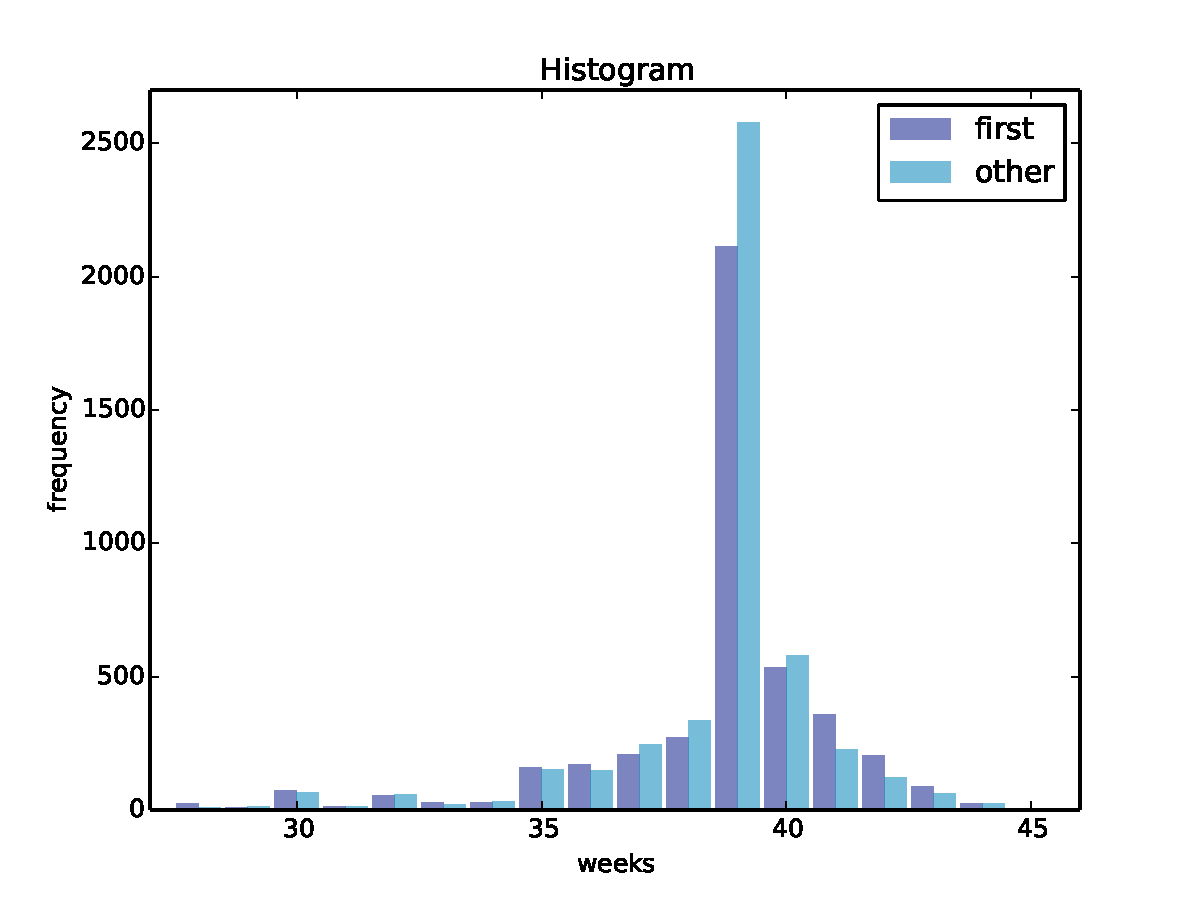
\includegraphics[height=2.5in]{figs/nsfg_hist.pdf}}
\caption{Histogram of pregnancy lengths.}
\label{nsfg_hist}
\end{figure}

Histograms are useful because they make the following features immediately
apparent:

\begin{itemize}

\item Mode: The most common value in a distribution is called the
  {\bf mode}.  In Figure~\ref{nsfg_hist} there is a clear mode at 39
  weeks.  In this case, the mode is the summary statistic that does
  the best job of describing the typical value.
\index{mode}

\item Shape: Around the mode, the distribution is asymmetric; it
  drops off quickly to the right and more slowly to the left.  From a
  medical point of view, this makes sense.  Babies are often born
  early, but seldom later than 42 weeks.  Also, the right side of the
  distribution is truncated because doctors often intervene after 42
  weeks.
\index{shape}

\item Outliers: Values far from the mode are called {\bf outliers}.
  Some of these are just unusual cases, like babies born at 30 weeks.
  But many of them are probably due to errors, either in the reporting
  or recording of data.
\index{outlier}

\end{itemize}

Although histograms make some features apparent, they are usually not
useful for comparing two distributions.  In this example, there are
fewer ``first babies'' than ``others,'' so some of the apparent
differences in the histograms are due to sample sizes.  We can
address this problem using PMFs.


\section{Representing PMFs}
\index{Pmf object}
\index{{\tt pmf.py}@{\tt Pmf.py}}

{\tt thinkstats2.py} provides a class called {\tt Pmf} that represents PMFs.
The notation can be confusing, but here it is: {\tt Pmf} is the
name of the class, I often use {\tt pmf} as a variable name, and in
this book, I use ``PMF'' to refer to the general concept
of a probability mass function, independent of my implementation.

To create a Pmf object, use {\tt MakePmfFromList}, which takes a list
of values:
%
\begin{verbatim}
>>> import thinkstats2
>>> pmf = thinkstats2.MakePmfFromList([1, 2, 2, 3, 5])
>>> print pmf
<thinkstats2.Pmf object at 0xb76cf68c>
\end{verbatim}

Pmf and Hist objects are similar in many ways.  The methods {\tt
  Values} and {\tt Items} work the same way for both types.  The
biggest difference is that a Hist maps from values to integer
counters; a Pmf maps from values to floating-point probabilities.

To look up the probability associated with a value, use {\tt Prob}:
%
\begin{verbatim}
>>> pmf.Prob(2)
0.4
\end{verbatim}

You can modify an existing Pmf by incrementing the probability
associated with a value:
%
\begin{verbatim}
>>> pmf.Incr(2, 0.2)
>>> pmf.Prob(2)
0.6
\end{verbatim}

Or you can multiply a probability by a factor:
%
\begin{verbatim}
>>> pmf.Mult(2, 0.5)
>>> pmf.Prob(2)
0.3
\end{verbatim}

If you modify a Pmf, the result may not be normalized; that is, the
probabilities may no longer add up to 1.  To check, you can call {\tt
  Total}, which returns the sum of the probabilities:
%
\begin{verbatim}
>>> pmf.Total()
0.9
\end{verbatim}

To renormalize, call {\tt Normalize}:
%
\begin{verbatim}
>>> pmf.Normalize()
>>> pmf.Total()
1.0
\end{verbatim}

Pmf objects provide a {\tt Copy} method so you can make
and modify a copy without affecting the original.

\begin{exercise}
According to Wikipedia, ``Survival analysis is a branch of statistics
which deals with death in biological organisms and failure in
mechanical systems;'' see \url{http://wikipedia.org/wiki/Survival_analysis}.
\index{survival analysis}

As part of survival analysis, it is often useful to compute the
remaining lifetime of, for example, a mechanical component.  If we
know the distribution of lifetimes and the age of the component,
we can compute the distribution of remaining lifetimes.

Write a function called {\tt RemainingLifetime} that takes a
Pmf of lifetimes and an age, and returns a new Pmf that represents
the distribution of remaining lifetimes.

\end{exercise}


\section{Plotting PMFs}
\index{plotting}
\index{PMF}

There are two common ways to plot Pmfs:

\begin{itemize}

\item To plot a Pmf as a bar graph, you can use {\tt pyplot.bar}
or {\tt myplot.Hist}.  Bar graphs are most useful if the number
of values in the Pmf is small.
\index{bar plot}
\index{plot!bar}

\item To plot a Pmf as a line, you can use {\tt pyplot.plot}
or {\tt myplot.Pmf}.  Line plots are most useful if there are
a large number of values and the Pmf is smooth.
\index{line plot}
\index{plot!line}

\end{itemize}

\begin{figure}
% descriptive.py
\centerline{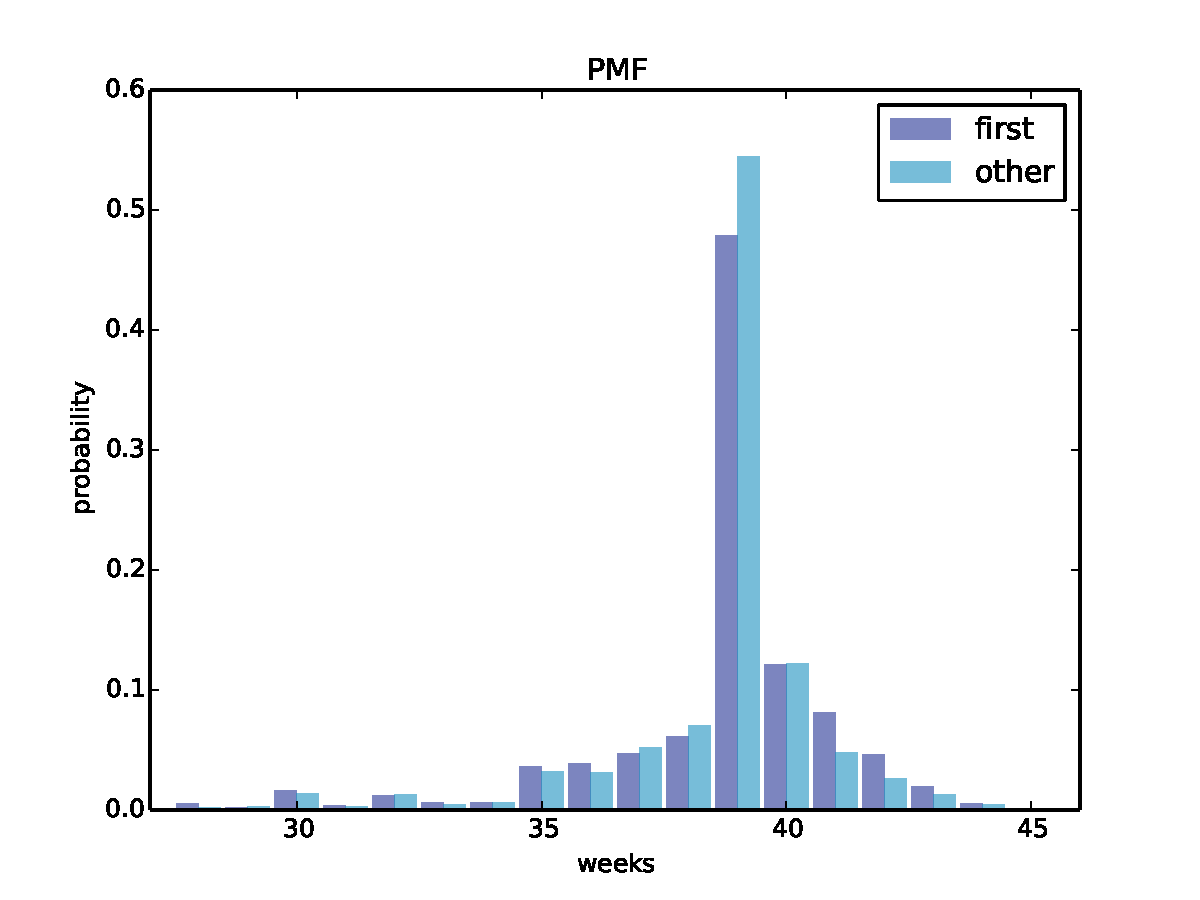
\includegraphics[height=2.5in]{figs/nsfg_pmf.pdf}}
\caption{PMF of pregnancy lengths.}
\label{nsfg_pmf}
\end{figure}
\index{pregnancy length}
\index{length!pregnancy}

Figure~\ref{nsfg_pmf} shows the PMF of pregnancy lengths as a bar
graph.  Using the PMF, we can see more clearly where the distributions
differ.  First babies seem to be less likely than others to arrive on
time (week 39) and more likely to be a late (weeks 41 and 42).

The code that generates the figures in this chapters is available from
\url{http://thinkstats2.com/descriptive.py}.  To run it, you will need the
modules it imports and the data from the NSFG (see
Section~\ref{nsfg}).
\index{National Survey of Family Growth}
\index{NSFG}
\index{{\tt descriptive.py}}

Note: {\tt pyplot} provides a function called {\tt hist} that
takes a sequence of values, computes the histogram and plots it.
Since I use {\tt Hist} objects, I usually don't use {\tt pyplot.hist}.



\section{Other visualizations}
\index{visualization}
\index{exploratory data analysis}

Histograms and PMFs are useful for exploratory data analysis;
once you have an idea what is going on, it is often useful to
design a visualization that focuses on the apparent effect.
\index{apparent effect}

In the NSFG data, the biggest differences in the distributions are
near the mode.  So it makes sense to zoom in on that part of the
graph, and to transform the data to emphasize differences.
\index{National Survey of Family Growth}
\index{NSFG}

Figure~\ref{nsfg_diffs} shows the difference between the PMFs for weeks
35--45.  I multiplied by 100 to express the differences in percentage
points.

\begin{figure}
% descriptive.py
\centerline{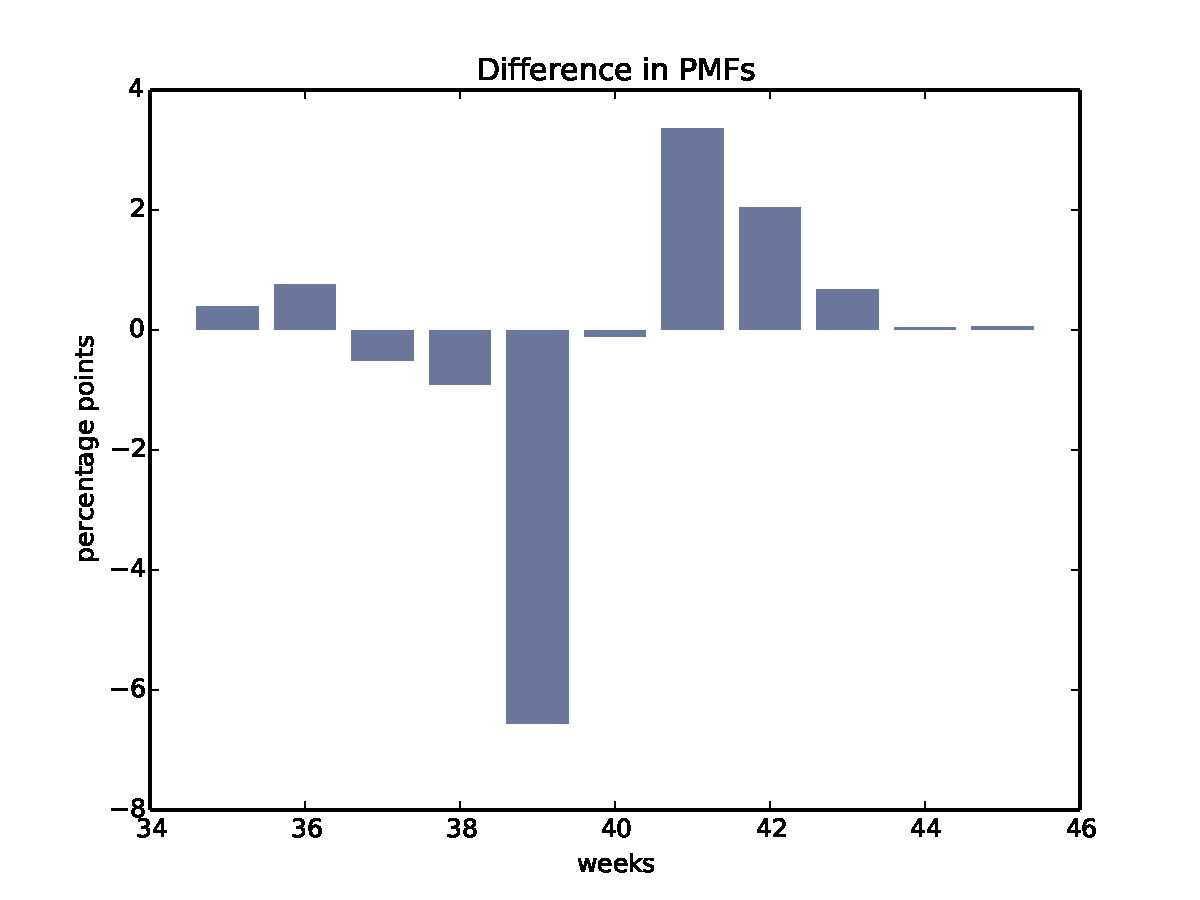
\includegraphics[height=2.5in]{figs/nsfg_diffs.pdf}}
\caption{Difference in percentage, by week.}
\label{nsfg_diffs}
\end{figure}

This figure makes the pattern clearer: first babies are
less likely to be born in week 39, and somewhat more likely
to be born in weeks 41 and 42.


\section{Relative risk}
\label{relative.risk}
\index{relative risk}

We started with the question, ``Do first babies arrive late?''  To
make that more precise, let's say that a baby is early if it is born
during Week 37 or earlier, on time if it is born during Week 38, 39 or
40, and late if it is born during Week 41 or later.  Ranges like these
that are used to group data are called {\bf bins}.
\index{bin}
\index{{\tt risk.py}}

\begin{exercise}
Create a file named {\tt risk.py}.
Write functions named {\tt ProbEarly}, {\tt ProbOnTime} and
{\tt ProbLate} that take a PMF and compute the fraction of births
that fall into each bin.  Hint: write a generalized function
that these functions call.

Make three PMFs, one for first babies, one for others, and one for
all live births.  For each PMF, compute the probability of being
born early, on time, or late.

One way to summarize data like this is with {\bf relative risk},
which is a ratio of two probabilities.  For example, the probability
that a first baby is born early is 18.2\%.  For other babies it is
16.8\%, so the relative risk is 1.08.  That means that first babies
are about 8\% more likely to be early.

Write code to confirm that result, then compute the relative risks of
being born on time and being late.  You can download a solution
from \url{http://thinkstats2.com/risk.py}.

\end{exercise}


\section{Means and averages}
\label{mean}

In the previous chapter, I mentioned three summary statistics---mean,
variance and median---without explaining what they are.  So before
we go any farther, let's take care of that.
\index{mean}
\index{average}
\index{descriptive statistics}
\index{summary statistics}

If you have a sample of $n$ values, $x_i$, the mean, $\xbar$, is
the sum of the values divided by the number of values; in other words
%
\[ \xbar = \frac{1}{n} \sum_i x_i \]
%
The words ``mean'' and ``average'' are sometimes used interchangeably,
but I will maintain this distinction:

\begin{itemize}

\item The ``mean'' of a sample is the summary statistic computed with
  the previous formula.

\item An ``average'' is one of several summary statistics you might
  choose to describe the typical value or the
  {\bf central tendency} of a sample.
\index{central tendency}

\end{itemize}

Sometimes the mean is a good description of a set of values.  For
example, apples are all pretty much the same size (at least the ones
sold in supermarkets).  So if I buy 6 apples and the total weight is 3
pounds, it would be a reasonable summary to say they are about a half
pound each.
\index{weight!pumpkin}

But pumpkins are more diverse.  Suppose I grow several varieties in my
garden, and one day I harvest three decorative pumpkins that are 1
pound each, two pie pumpkins that are 3 pounds each, and one Atlantic
Giant\textregistered~pumpkin that weighs 591 pounds.  The mean of
this sample is 100 pounds, but if I told you ``The average pumpkin
in my garden is 100 pounds,'' that would be wrong, or at least
misleading.  In this example, there is no meaningful average because
there is no typical pumpkin.
\index{pumpkin}



\section{Variance}
\index{variance}

If there is no single number that summarizes pumpkin weights,
we can do a little better with two numbers: mean and {\bf variance}.

In the same way that the mean is intended to describe the central
tendency, variance is intended to describe the {\bf spread}.
The variance of a set of values is
%
\[ S^2 = \frac{1}{n} \sum_i (x_i - \xbar)^2 \]
%
The term $x_i - \xbar$ is called the ``deviation from the mean,'' so
variance is the mean squared deviation, which is why it is denoted
with exponent 2.  The square root of variance, $S$, is the
{\bf standard deviation}.  \index{deviation} \index{standard
  deviation}

By itself, variance is hard to interpret.  One problem is that the
units are strange; in this case the measurements are in pounds, so the
variance is in pounds squared.  Standard deviation is more meaningful;
in this example the units are pounds.

If you have prior experience, you might have seen a formula for
variance with $n-1$ in the denominator, rather than $n$.  This
statistic is used to
estimate the variance in a population using a sample.  We will come
back to this in Chapter~\ref{estimation}.  \index{sample variance}


\begin{exercise}
%
\index{mean}
\index{variance}
\index{PMF}
%
In Section~\ref{mean} we computed the mean of a sample by adding up
the elements and dividing by n.  If you are given a PMF, you can
still compute the mean, but the process is slightly different:
%
\[ \xbar = \sum_i p_i x_i \]
%
where the $x_i$ are the unique values in the PMF and $p_i=PMF(x_i)$.
Similarly, you can compute variance like this:
%
\[ S^2 = \sum_i p_i (x_i - \xbar)^2\]
% 
Write functions called {\tt PmfMean} and {\tt PmfVar} that take a
Pmf object and compute the mean and variance.  To test these methods,
check that they are consistent with the methods {\tt Mean} and {\tt
  Var} provided by {\tt Pmf}.
\index{{\tt pmf.py}@{\tt Pmf.py}}

\end{exercise}


\section{Outliers}
\index{outlier}

Outliers are values that are far from the central tendency.  Outliers
might be caused by errors in collecting or processing the data, or
they might be correct but unusual measurements.  It is always a good
idea to check for outliers, and sometimes it is useful and appropriate
to discard them.

%weeks  count
%0      1
%4      1
%9      1
%13     1
%17     2
%18     1
%19     1
%20     1
%21     2
%22     7

In the list of pregnancy lengths for live births, the 10 lowest values
are \{0, 4, 9, 13, 17, 17, 18, 19, 20, 21\}.  Values below 20
weeks are certainly errors, and values higher than 30 weeks are
probably legitimate.  But values in between are
hard to interpret.
\index{pregnancy length}
\index{length!pregnancy}

On the other end, the highest values are:
%
\begin{verbatim}
weeks  count
43     148
44     46
45     10
46     1
47     1
48     7
50     2
\end{verbatim}

Again, some values are almost certainly errors,
but it is hard to know for sure.  One option is to {\bf trim} the data
by discarding some fraction of the highest and lowest values (see
\url{http://wikipedia.org/wiki/Truncated_mean}).
\index{trimmed mean}
\index{mean!trimmed}
\index{truncated mean}
\index{mean!truncated}


\section{Reporting results}

At this point we have explored the data and seen several apparent
effects.  For now, let's assume that these effects are real (but let's
remember that it's an assumption).  How should we report these
results?

The answer might depend on who is asking the question.  For example, a
scientist might be interested in any (real) effect, no matter how
small.  A doctor might only care about effects that are {\bf
  clinically significant}; that is, differences that affect treatment
decisions.  A pregnant woman might be interested in results that are
relevant to her, like the probability of delivering early or late.
\index{clinically significant}
\index{significance}

How you report results also depends on your goals.  If you are
trying to demonstrate the significance of an effect, you might choose
summary statistics, like relative risk, that emphasize differences.
If you are trying to reassure a patient, you might choose statistics
that put the differences in context.

\begin{exercise}
Reusing code from {\tt survey.py} and {\tt first.py}, compute the
standard deviation of gestation time for first babies and others.
Does it look like the spread is the same for the two groups?
\index{{\tt survey.py}}
\index{{\tt first.py}}

How big is the difference in the means compared to these standard
deviations?  What does this comparison suggest about the statistical
significance of the difference?
\end{exercise}

\begin{exercise}
Based on the results from the previous exercises, suppose you were
asked to summarize what you learned about whether first
babies arrive late.

Which summary statistics would you use if you wanted to get a story
on the evening news?  Which ones would you use if you wanted to
reassure an anxious patient?
\index{Adams, Cecil}
\index{Straight Dope, The}

Finally, imagine that you are Cecil Adams, author of {\it The Straight
  Dope} (\url{http://straightdope.com}), and your job is to answer the
question, ``Do first babies arrive late?''  Write a paragraph that
uses the results in this chapter to answer the question clearly,
precisely, and accurately.

\end{exercise}



\section{Glossary}

\begin{itemize}

\item central tendency: A characteristic of a sample or population;
intuitively, it is the most average value. 
\index{central tendency}

\item spread: A characteristic of a sample or population;
intuitively, it describes how much variability there is.
\index{spread}

\item variance: A summary statistic often used to quantify spread.
\index{variance}

\item standard deviation: The square root of variance, also used
as a measure of spread.
\index{standard deviation}

\item frequency: The number of times a value appears in a sample.
\index{frequency}

\item histogram: A mapping from values to frequencies, or a graph
that shows this mapping.
\index{histogram}

\item probability: A frequency expressed as a fraction of the sample
size.
\index{probability}

\item normalization: The process of dividing a frequency by a sample
size to get a probability.
\index{normalization}

\item distribution: A summary of the values that appear in a sample
and the frequency, or probability, of each.
\index{distribution}

\item PMF: Probability mass function: a representation of a distribution
as a function that maps from values to probabilities.
\index{PMF}

\item mode: The most frequent value in a sample.
\index{mode}

\item outlier: A value far from the central tendency.
\index{outlier}

\item trim: To remove outliers from a dataset.
\index{trim}

\item bin: A range used to group nearby values.
\index{bin}

\item relative risk: A ratio of two probabilities, often used to measure
a difference between distributions.
\index{relative risk}

\item conditional probability: A probability computed under the assumption
that some condition holds.
\index{conditional probability}

\item clinically significant: A result, like a difference between groups,
that is relevant in practice.
\index{clinically significant}

\end{itemize}


\chapter{Cumulative distribution functions}
\label{cumulative}

\section{The class size paradox}
\index{class size}

At many American colleges and universities, the student-to-faculty
ratio is about 10:1.  But students are often surprised to discover
that their average class size is bigger than 10.  There
are two reasons for the discrepancy:

\begin{itemize}

\item Students typically take 4--5 classes per semester, but
professors often teach 1 or 2.

\item The number of students who enjoy a small class is small,
but the number of students in a large class is (ahem!) large.

\end{itemize}

The first effect is obvious (at least once it is pointed out);
the second is more subtle.  So let's look at an example.  Suppose
that a college offers 65 classes in a given semester, with the
following distribution of sizes:
%
\begin{verbatim}
 size      count
 5- 9          8
10-14          8
15-19         14
20-24          4
25-29          6
30-34         12
35-39          8
40-44          3
45-49          2
\end{verbatim}

If you ask the Dean for the average class size, he would
construct a PMF, compute the mean, and report that the
average class size is 24.

But if you survey a group of students, ask them how many
students are in their classes, and compute the mean, you would
think that the average class size was higher.

\begin{exercise}
Build a PMF of these data and compute the mean as perceived by the
Dean.  Since the data have been grouped in bins, you can use the
mid-point of each bin.
\index{PMF}

Now find the distribution of class sizes as perceived by students
and compute its mean.  

Suppose you want to find the distribution of class sizes at a
college, but you can't get reliable data from the Dean.
An alternative is to choose a random sample of students and ask them
the number of students in each of their classes.  Then you could compute
the PMF of their responses.
\index{bias!oversampling}
\index{oversampling}

The result would be biased because large classes
would be oversampled, but you could estimate the actual
distribution of class sizes by applying an appropriate transformation
to the observed distribution.

Write a function called \verb"UnbiasPmf" that takes the PMF of the
observed values and returns a new Pmf object that estimates the
distribution of class sizes.

You can download a solution to this problem from
\url{http://thinkstats2.com/class_size.py}.
\index{{\tt class\_size.py}}

\end{exercise}


\begin{exercise}
\label{relay}

In most foot races, everyone starts at the same time.  If you are a
fast runner, you usually pass a lot of people at the beginning of the
race, but after a few miles everyone around you is going at the same
speed.
\index{relay race}
\index{bias!oversampling}
\index{oversampling}

When I ran a long-distance (209 miles) relay race for the first
time, I noticed an odd phenomenon: when I overtook another runner, I
was usually much faster, and when another runner overtook me, he was
usually much faster.

At first I thought that the distribution of speeds might be bimodal;
that is, there were many slow runners and many fast runners, but few
at my speed.

Then I realized that I was the victim of selection bias.  The race
was unusual in two ways: it used a staggered start, so teams started
at different times; also, many teams included runners at different
levels of ability.
\index{bias!selection}
\index{selection bias}

As a result, runners were spread out along the course with little
relationship between speed and location.  When I started running my
leg, the runners near me were (pretty much) a random sample of the
runners in the race.

So where does the bias come from?  During my time on the course, the
chance of overtaking a runner, or being overtaken, is proportional to
the difference in our speeds.  To see why, think about the extremes.
If another runner is going at the same speed as me, neither of us will
overtake the other.  If someone is going so fast that they cover the
entire course while I am running, they are certain to overtake me.

Write a function called {\tt BiasPmf} that takes a Pmf representing
the actual distribution of runners' speeds, and the speed of a running
observer, and returns a new Pmf representing the distribution of
runners' speeds as seen by the observer.

To test your function, get the distribution of speeds from a
normal road race (not a relay).  I wrote a program that reads the
results from the James Joyce Ramble 10K in Dedham MA and converts the
pace of each runner to MPH.  Download it from
\url{http://thinkstats2.com/relay.py}.  Run it and look at the PMF of
speeds.
\index{{\tt relay.py}}
\index{{\tt relay\_soln.py}}

Now compute the distribution of speeds you would observe if you ran a
relay race at 7.5 MPH with this group of runners.  You can download a
solution from \url{http://thinkstats2.com/relay_soln.py}

\end{exercise}


\section{The limits of PMFs}
\index{PMF}

PMFs work well if the number of values is small.  But as the
number of values increases, the probability associated with each value
gets smaller and the effect of random noise increases.

For example, we might be interested in the distribution of birth
weights.  In the NSFG data, the variable \verb"totalwgt_oz" records
weight at birth in ounces.  Figure~\ref{nsfg_birthwgt_pmf} shows the
PMF of these values for first babies and others.
\index{National Survey of Family Growth}
\index{NSFG}
\index{birth weight}
\index{weight!birth}

\begin{figure}
% cumulative.py
\centerline{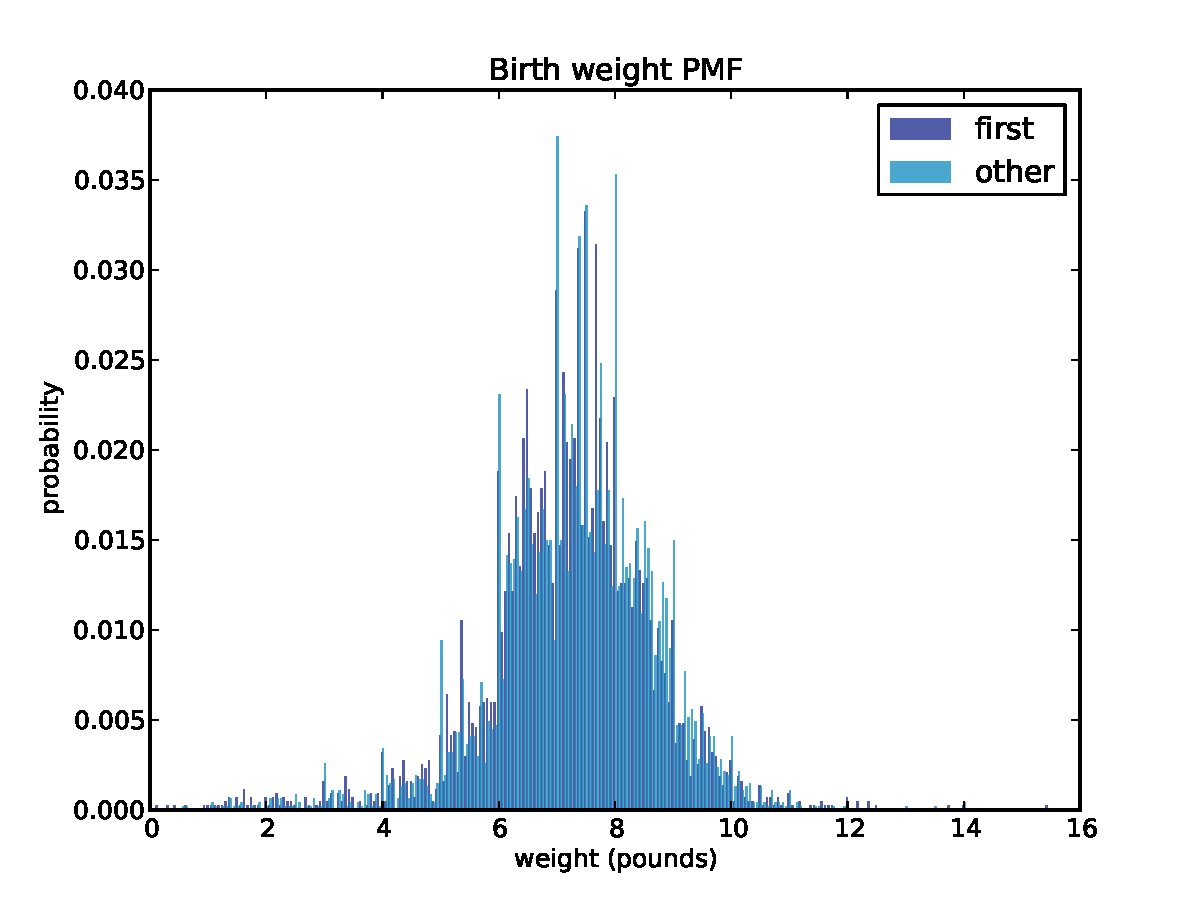
\includegraphics[height=2.5in]{figs/nsfg_birthwgt_pmf.pdf}}
\caption{PMF of birth weights.  This figure shows a limitation
of PMFs: they are hard to compare.}
\label{nsfg_birthwgt_pmf}
\end{figure}

Overall, these distributions resemble the familiar ``bell curve,'' with
many values near the mean and a few values much higher and lower.

But parts of this figure are hard to interpret.  There are many spikes
and valleys, and some apparent differences between the distributions.
It is hard to tell which of these features are significant.  Also, it
is hard to see overall patterns; for example, which distribution do
you think has the higher mean?
\index{binning}

These problems can be mitigated by binning the data;
that is, dividing the domain into non-overlapping intervals and counting
the number of values in each bin.  Binning can be useful, but it is
tricky to get the size of the bins right.  If they are big enough to
smooth out noise, they might also smooth out useful information.

An alternative that avoids these problems is the {\bf cumulative
distribution function}, or {\bf CDF}.  But before we can get to that,
we have to talk about percentiles.
\index{cumulative distribution function}
\index{CDF}


\section{Percentiles}
\index{percentile rank}

If you have taken a standardized test, you probably got your
results in the form of a raw score and a {\bf percentile rank}.
In this context, the percentile rank is the fraction of people who
scored lower than you (or the same).  So if you are ``in the 90th
percentile,'' you did as well as or better than 90\% of the people who
took the exam.

Here's how you could compute the percentile rank of a value,
\verb"your_score", relative to the scores in the sequence {\tt
  scores}:
%
\begin{verbatim}
def PercentileRank(scores, your_score):
    count = 0
    for score in scores:
        if score <= your_score:
            count += 1

    percentile_rank = 100.0 * count / len(scores)
    return percentile_rank
\end{verbatim}
%
% see score_example.py
%
For example, if the scores in the sequence were 55, 66, 77, 88 and 99,
and you got the 88, then your percentile rank would be {\tt 100 * 4 / 5}
which is 80.

If you are given a value, it is easy to find its percentile rank; going
the other way is slightly harder.  If you are given a percentile rank
and you want to find the corresponding value, one option is to
sort the values and search for the one you want:
%
\begin{verbatim}
def Percentile(scores, percentile_rank):
    scores.sort()
    for score in scores:
        if PercentileRank(scores, score) >= percentile_rank:
            return score
\end{verbatim}

The result of this calculation is a {\bf percentile}.  For example,
the 50th percentile is the value with percentile rank 50.  In the
distribution of exam scores, the 50th percentile is 77.
\index{percentile}

\begin{exercise}
This implementation of {\tt Percentile} is not very efficient.  A
better approach is to use the percentile rank to compute the index of
the corresponding percentile.  Write a version of {\tt Percentile} that
uses this algorithm.

You can download a solution from \url{http://thinkstats2.com/score_example.py}.
\index{{\tt score\_example.py}}

\end{exercise}

\begin{exercise}
Optional: If you only want to compute one percentile, it is not
efficient to sort the scores.  A better option is the selection
algorithm, which you can read about at
\url{http://wikipedia.org/wiki/Selection_algorithm}.
\index{selection algorithm}

Write (or find) an implementation of the selection algorithm and use
it to write an efficient version of {\tt Percentile}.

\end{exercise}


\section{Cumulative distribution functions}
\index{cumulative distribution function}
\index{CDF}

Now that we understand percentiles, we are ready to tackle the
cumulative distribution function (CDF).  The CDF is the function that
maps values to their percentile rank in a distribution.

The CDF is a function of $x$, where $x$ is any value that might appear
in the distribution.  To evaluate $\CDF(x)$ for a particular value of
$x$, we compute the fraction of the values in the sample less than (or
equal to) $x$.

Here's what that looks like as a function that takes a sample,
{\tt t}, and a value, {\tt x}:
%
\begin{verbatim}
def Cdf(t, x):
    count = 0.0
    for value in t:
        if value <= x:
            count += 1.0

    prob = count / len(t)
    return prob
\end{verbatim}

This function should look familiar; it is almost identical to {\tt
  PercentileRank}, except that the result is in a probability in the
range 0--1 rather than a percentile rank in the range 0--100.

As an example, suppose a sample has the values \{1, 2, 2, 3, 5\}.
Here are some values from its CDF:

\[ CDF(0) = 0 \]

\[ CDF(1) = 0.2\]

\[ CDF(2) = 0.6\]

\[ CDF(3) = 0.8\]

\[ CDF(4) = 0.8\]

\[ CDF(5) = 1\]

We can evaluate the CDF for any value of $x$, not just
values that appear in the sample.
If $x$ is less than the smallest value in the sample, $\CDF(x)$ is 0.
If $x$ is greater than the largest value, $\CDF(x)$ is 1.

\begin{figure}
% cumulative.py
\centerline{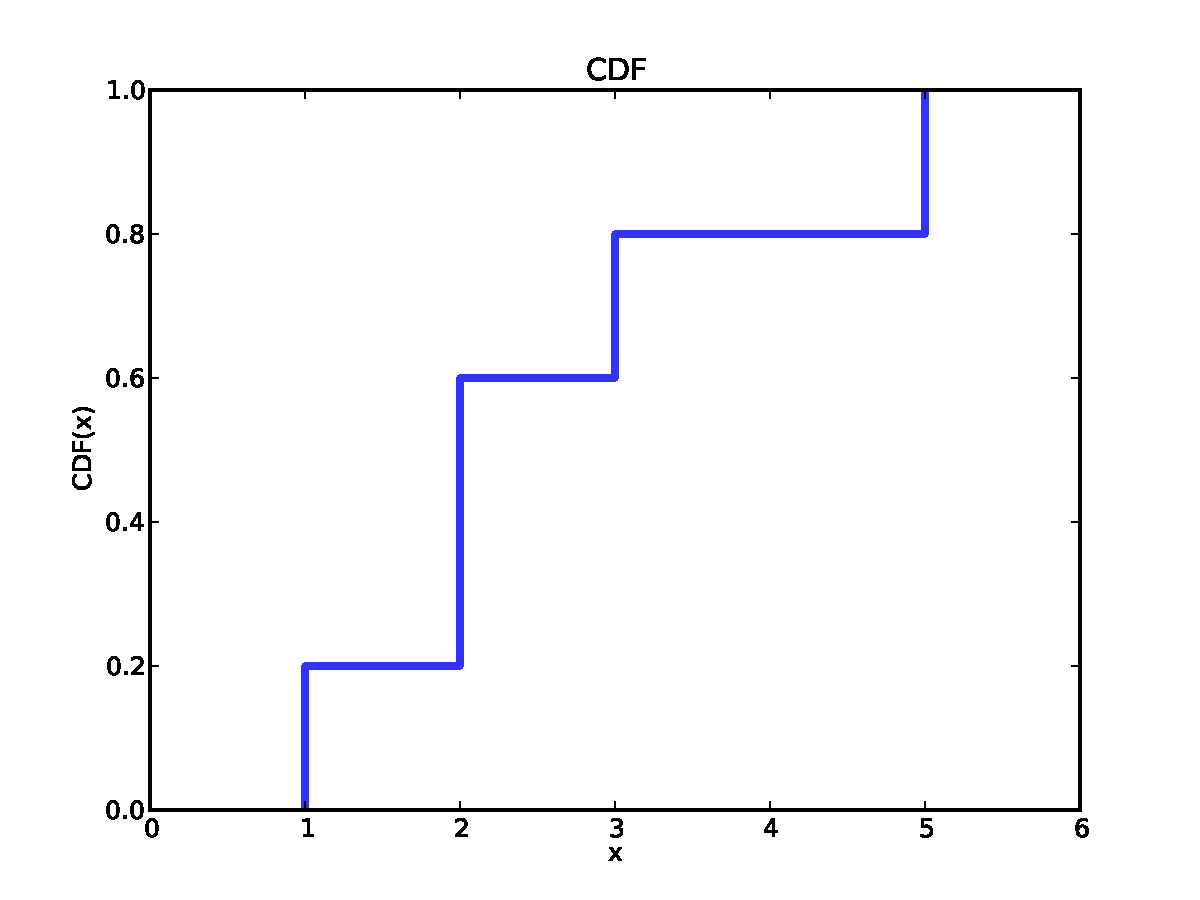
\includegraphics[height=2.5in]{figs/example_cdf.pdf}}
\caption{Example of a CDF.}
\label{example_cdf}
\end{figure}

Figure~\ref{example_cdf} is a graphical representation of this CDF.
The CDF of a sample is a step function.  In the next chapter we
will see distributions whose CDFs are continuous functions.  


\section{Representing CDFs}
\index{{\tt cdf.py}@{\tt Cdf.py}}
\index{Cdf object}

I have written a module called {\tt Cdf} that provides a class named
{\tt Cdf} that represents CDFs.  You can read the documentation of
this module at \url{http://thinkstats2.com/Cdf.html} and you can download it
from \url{http://thinkstats2.com/Cdf.py}.

Cdfs are implemented with two sorted lists: {\tt xs}, which contains
the values, and {\tt ps}, which contains the probabilities.  The
most important methods Cdfs provide are:

\begin{itemize}

\item {\tt Prob(x)}: Given a value $x$, computes the probability $p = \CDF(x)$.

\item {\tt Value(p)}: Given a probability $p$, computes the
corresponding value, $x$; that is, the inverse CDF of $p$.

\end{itemize}

Because {\tt xs} and {\tt ps} are sorted, these operations can use the
bisection algorithm, which is efficient.  The run time is proportional
to the logarithm of the number of values; see
\url{http://wikipedia.org/wiki/Time_complexity}.
\index{bisection algorithm}

Cdfs also provide {\tt Render}, which returns two lists, {\tt xs} and
{\tt ps}, suitable for plotting the CDF.  Because the CDF is a
step function, these lists have two elements for each unique
value in the distribution.

The Cdf module provides several functions for making Cdfs, including
{\tt MakeCdfFromList}, which takes a sequence of values
and returns their Cdf.

Finally, {\tt myplot.py} provides functions named {\tt Cdf} and
{\tt Cdfs} that plot Cdfs as lines.
\index{{\tt myplot.py}}

\begin{exercise}
Download {\tt Cdf.py} and \verb"relay.py" (see
Exercise~\ref{relay}) and generate a plot that shows the CDF of
running speeds.  Which gives you a better sense of the shape of the
distribution, the PMF or the CDF?  You can download a solution
from \url{http://thinkstats2.com/relay_cdf.py}.
\index{{\tt cdf.py}@{\tt Cdf.py}}
\index{{\tt relay\_cdf.py}}

\end{exercise}


\section{Back to the survey data}
\label{birth_weights}
\index{National Survey of Family Growth}
\index{NSFG}
\index{birth weight}
\index{weight!birth}

Figure~\ref{nsfg_birthwgt_cdf} shows the CDFs of birth weight for
first babies and others in the NSFG dataset.

\begin{figure}
% cumulative.py
\centerline{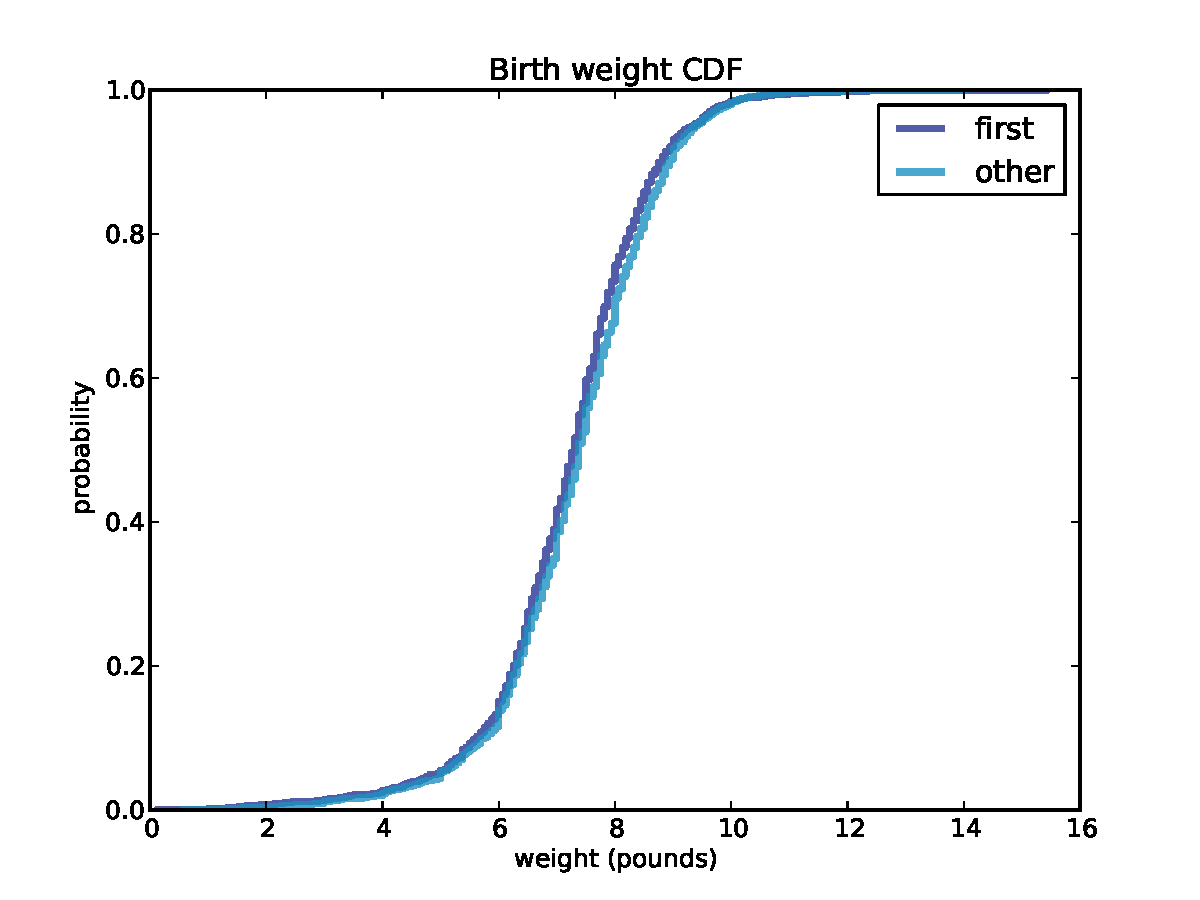
\includegraphics[height=2.5in]{figs/nsfg_birthwgt_cdf.pdf}}
\caption{CDF of birth weights.}
\label{nsfg_birthwgt_cdf}
\end{figure}

This figure makes the shape of the distributions, and the differences
between them, much clearer.  We can see that first babies are slightly
lighter throughout the distribution, with a larger discrepancy above 
the mean.
\index{shape}

%\begin{exercise}

%In the figure above, you might notice
%a sequence of equally-spaced values with higher frequency than
%their neighbors.  See if you can figure out what is going on.
%Hint: look at the PMF of \verb"birthwgt_oz".

%\end{exercise}

\begin{exercise}
How much did you weigh at birth?  If you don't know, call your mother
or someone else who knows.  Using the pooled data (all live births),
compute the distribution of birth weights and use it to find your
percentile rank.  If you were a first baby, find your percentile rank
in the distribution for first babies.  Otherwise use the distribution
for others.  If you are in the 90th percentile or higher, call your
mother back and apologize.

\end{exercise}

\begin{exercise}
Suppose you and your classmates compute the percentile rank of your
birth weights and then compute the CDF of the percentile ranks.  What do
you expect it to look like?  Hint: what fraction of the class do you
expect to be above the median?
\index{birth weight}
\index{weight!birth}

\end{exercise}


\section{Conditional distributions}
\index{conditional distribution}
\index{distribution!conditional}

A {\bf conditional distribution} is the distribution of a subset of
the data which is selected according to a condition.

For example, if you are above average in weight, but way above average
in height, then you might be relatively light for your height.  Here's
how you could make that claim more precise.

\begin{enumerate}

\item Select a cohort of people who are the same height as you (within
some range).
\index{cohort}

\item Find the CDF of weight for those people.

\item Find the percentile rank of your weight in that distribution.

\end{enumerate}

Percentile ranks are useful for comparing measurements from
different tests, or tests applied to different groups.
\index{percentile rank}
\index{rank!percentile}

For example, people who compete in foot races are usually grouped by
age and gender.  To compare people in different groups, you can convert
race times to percentile ranks.

\begin{exercise}
I recently ran the James Joyce Ramble 10K
in Dedham MA.  The results are available from
\url{http://coolrunning.com/results/10/ma/Apr25_27thAn_set1.shtml}.
Go to that page and find my results.  I came in 97th in a field
of 1633, so what is my percentile rank in the field?
\index{James Joyce Ramble}
\index{race time}

In my division (M4049 means ``male between 40 and 49 years of age'')
I came in 26th out of 256.  What is my percentile rank in my division?

If I am still running in 10 years (and I hope I am), I will be in
the M5059 division.  Assuming that my percentile rank in my division
is the same, how much slower should I expect to be?

I maintain a friendly rivalry with a student who is in the
F2039 division.  How fast does she have to run her next 10K to
``beat'' me in terms of percentile ranks?

\end{exercise}


\section{Random numbers}
\label{random}
\index{random number}

CDFs are useful for generating random numbers with a given
distribution.  Here's how:

\begin{itemize}

\item Choose a random probability in the range 0--1.

\item Use {\tt Cdf.Value} to find the value in the distribution
that corresponds to the probability you chose.

\end{itemize}

It might not be obvious why this works, but since it is easier
to implement than to explain, let's try it out.

\begin{exercise}
Write a function called {\tt Sample}, that takes a Cdf and
an integer, n, and returns a list of $n$values chosen at
random from the Cdf.  Hint: use {\tt random.random}.
You will find a solution to this exercise in {\tt Cdf.py}.
\index{inverse CDF algorithm}
\index{{\tt cdf.py}@{\tt Cdf.py}}

Using the distribution of birth weights from the NSFG, generate a
random sample with 1000 elements.  Compute the CDF of the sample.
Make a plot that shows the original CDF and the CDF of the random
sample.  For large values of n, the distributions should be
the same.
\index{birth weight}
\index{weight!birth}
\index{National Survey of Family Growth}
\index{NSFG}

\end{exercise}

This process, generating a random sample based on a measured sample,
is called {\bf resampling}.
\index{resampling}
\index{sampling}
\index{replacement, sampling}

There are two ways to draw a sample from a population: with and
without replacement.  If you imagine drawing marbles from an
urn,\footnote{The marbles-in-an-urn scenario is a standard model for
  random sampling processes (see
  \url{http://wikipedia.org/wiki/Urn_problem}).} ``replacement'' means
putting the marbles back as you go (and stirring), so the population
is the same for every draw.  ``Without replacement,'' means that each
marble can only be drawn once, so the remaining population is
different after each draw.

In Python, sampling with replacement can be implemented with
{\tt random.random} to choose a percentile rank, or {\tt random.choice}
to choose an element from a sequence.  Sampling without replacement
is provided by {\tt random.sample}.
\index{random module}

\begin{exercise}
The numbers generated by {\tt random.random} are supposed to be
uniform between 0 and 1; that is, every value in the range
should have the same probability.

Generate 1000 numbers from {\tt random.random} and plot their
PMF and CDF.  Can you tell whether they are uniform?

You can read about the uniform distribution at
\url{http://wikipedia.org/wiki/Uniform_distribution_(discrete)}.
\index{uniform distribution}
\index{distribution!uniform}

\end{exercise}


\section{Summary statistics revisited}
\index{summary statistic}
\index{interquartile range}
\index{quartile}
\index{percentile}
\index{median}
\index{central tendency}
\index{spread}

Once you have computed a CDF, it is easy to compute other summary
statistics.  The median is just the 50th percentile.\footnote{You might
see other definitions of the median.  They all have pros and cons.}
The 25th and 75th percentiles are often used to check whether
a distribution is symmetric, and their difference, which is called
the {\bf interquartile range}, measures the spread.

\begin{exercise}
Write a function called {\tt Median} that takes a Cdf and computes the
median, and one called {\tt Interquartile} that computes
the interquartile range.

Compute the 25th, 50th, and 75th percentiles of the birth weight
CDF.  Do these values suggest that the distribution is symmetric?
\index{symmetric}
\index{birth weight}
\index{weight!birth}

\end{exercise}


\section{Glossary}

\begin{itemize}

\item percentile rank: The percentage of values in a distribution that are
less than or equal to a given value.
\index{percentile rank}

\item CDF: Cumulative distribution function, a function that maps
  from values to their percentile ranks.
\index{CDF}

\item percentile: The value associated with a given percentile rank.
\index{percentile}

\item conditional distribution: A distribution computed under the assumption
that some condition holds.
\index{conditional distribution}

\item resampling: The process of generating a random sample from a
distribution that was computed from a sample.
\index{resampling}

\item replacement: During a sampling process, ``replacement'' indicates
that the population is the same for every sample.  ``Without replacement''
indicates that each element can be selected only once.
\index{replacement}

\item interquartile range: A measure of spread, the difference between
the 75th and 25th percentiles.
\index{interquartile range}

\end{itemize}


\chapter{Modeling distributions}
\label{analytic}
\index{analytic distribution}
\index{distribution!analytic}
\index{empirical distribution}
\index{distribution!empirical}

The distributions we have used so far are called {\bf
  empirical distributions} because they are based on empirical
observations, which are necessarily finite samples.

The alternative is an {\bf analytic distribution}, which is
characterized by a CDF that is a analytic function (as opposed to a
step function).  Many real world phenomena can be approximated by
analytic distributions.


\section{The exponential distribution}
\index{exponential distribution}
\index{distribution!exponential}

\begin{figure}
% continuous.py
\centerline{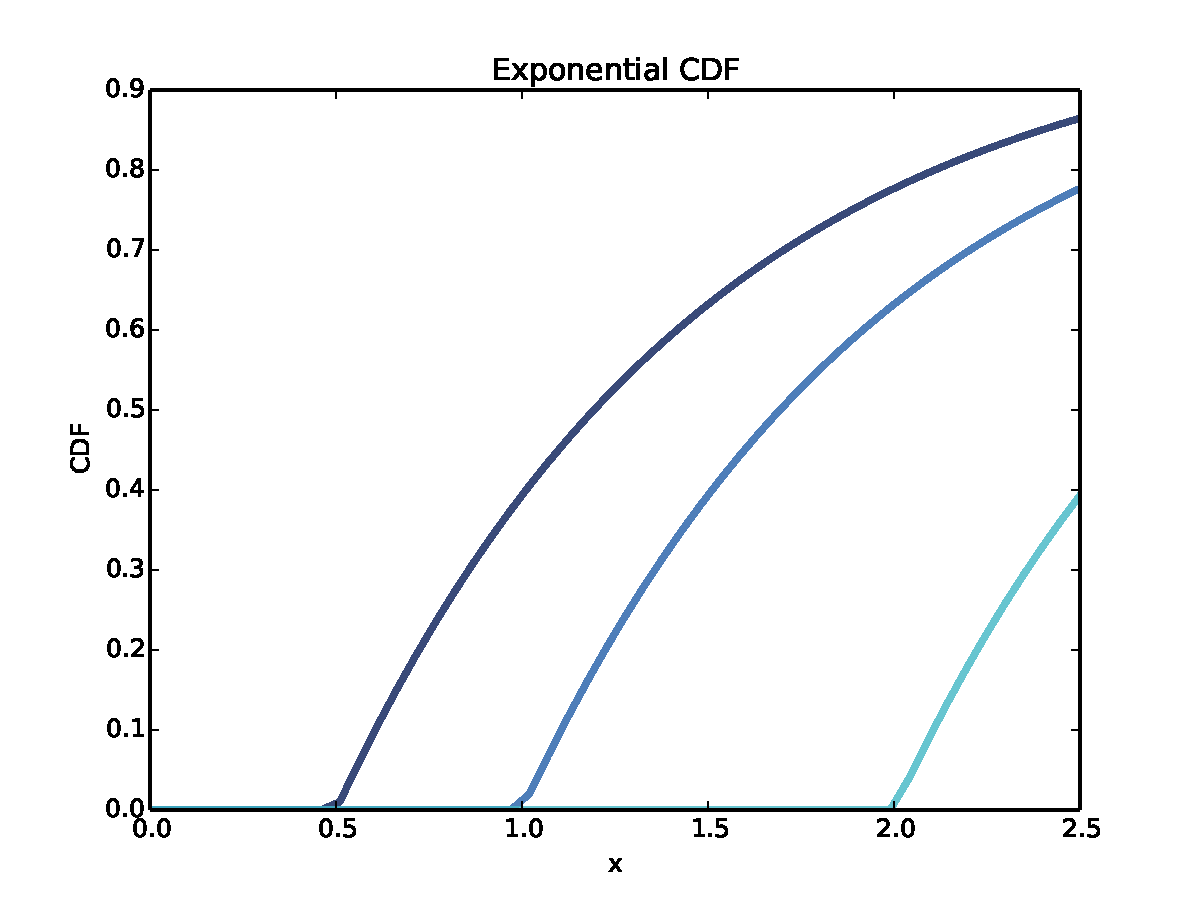
\includegraphics[height=2.5in]{figs/expo_cdf.pdf}}
\caption{CDF of exponential distribution.}
\label{expo_cdf}
\end{figure}

I'll start with the exponential distribution because it is
easy to work with.  In the real world, exponential distributions
come up when we look at a series of events and measure the
times between events, which are called {\bf interarrival times}.
If the events are equally likely to occur at any time, the distribution
of interarrival times tends to look like an exponential distribution.
\index{interarrival time}

The CDF of the exponential distribution is:
%
\[ CDF(x) = 1 - e^{-\lambda x} \]
%
The parameter, $\lambda$, determines the shape of the
distribution.  Figure~\ref{expo_cdf} shows what this CDF looks like with
$\lambda = 2$.
\index{parameter}

The mean of an exponential distribution is $1/\lambda$, so
the mean of this distribution is 0.5.  The median is $ln(2)/\lambda$,
which is roughly 0.35.  \index{mean} \index{median} \index{Australia}
\index{Brisbane}

To see an example of a distribution that is approximately exponential,
we will look at the interarrival time of babies.
On December 18, 1997, 44 babies were born in a hospital in Brisbane,
Australia.\footnote{This example is based on information and data from
  Dunn, ``A Simple Dataset for Demonstrating Common Distributions,''
  Journal of Statistics Education v.7, n.3 (1999).}  The times of
birth for all 44 babies were reported in the local paper; you can
download the data from \url{http://thinkstats2.com/babyboom.dat}.
\index{birth time}

Figure~\ref{interarrival_cdf} shows the CDF of the interarrival times
in minutes.  It seems to have the general shape of an exponential
distribution, but how can we tell?
\index{complementary CDF}
\index{CDF!complementary}
\index{CCDF}

One way is to plot the complementary CDF, $1 - CDF(x)$, on a
log-y scale.  For data from an exponential distribution, the result
is a straight line.  Let's see why that works.

If you plot the complementary CDF (CCDF) of a dataset that you think is
exponential, you expect to see a function like:
%
\[ y \approx e^{-\lambda x} \]
%
Taking the log of both sides yields:
%
\[ \log y \approx -\lambda x\]
%
So on a log-y scale the CCDF is a straight line
with slope $-\lambda$.
\index{logarithmic scale}
\index{complementary CDF}
\index{CDF!complementary}
\index{CCDF}

\begin{figure}
% babyboom.py
\centerline{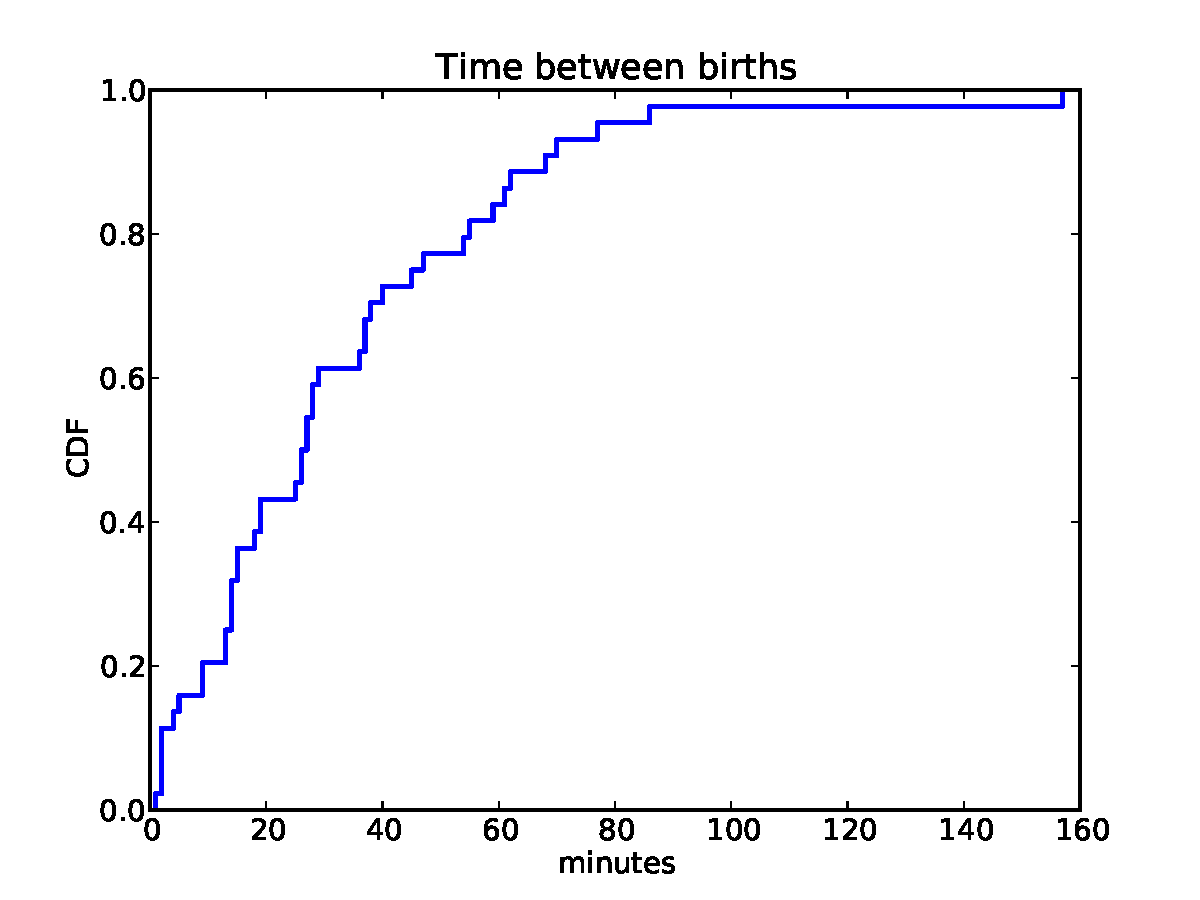
\includegraphics[height=2.5in]{figs/interarrivals.pdf}}
\caption{CDF of interarrival times}
\label{interarrival_cdf}
\end{figure}

Figure~\ref{interarrival_ccdf} shows the CCDF of the interarrivals on
a log-y scale.  It is not exactly straight, which suggests that the
exponential distribution is only an approximation.  Most likely the
underlying assumption---that a birth is equally likely at any time of
day---is not exactly true.  But for most purposes the exponential
distribution would be a reasonable model of this data.  And if we
think this simplification is reasonable, we can summarize the distribution
with a single parameter, $\lambda$.

\begin{exercise}
For small values of n, we don't expect an empirical distribution
to fit a analytic distribution exactly.  One way to evaluate
the quality of fit is to generate a sample from a analytic
distribution and see how well it matches the data.
\index{empirical distribution}
\index{distribution!empirical}
\index{random module}

The function {\tt expovariate} in the {\tt random} module generates
random values from an exponential distribution with a given value of
$\lambda$.  Use it to generate 44 values from an exponential
distribution with mean 32.6.  Plot the CCDF on a log-y scale and
compare it to Figure~\ref{interarrival_ccdf}.
\index{pyplot}

Hint: You can use the function {\tt pyplot.yscale} to plot the $y$ axis
on a log scale.

\end{exercise}

\begin{exercise}
Collect the birthdays of the students in your class, sort them, and
compute the interarrival times in days.  Plot the CDF of the interarrival
times and the CCDF on a log-y scale.  Does it look like
an exponential distribution?
\index{exponential distribution}
\index{distribution!exponential}
\index{birthday}

\end{exercise}


\begin{figure}
% babyboom.py
\centerline{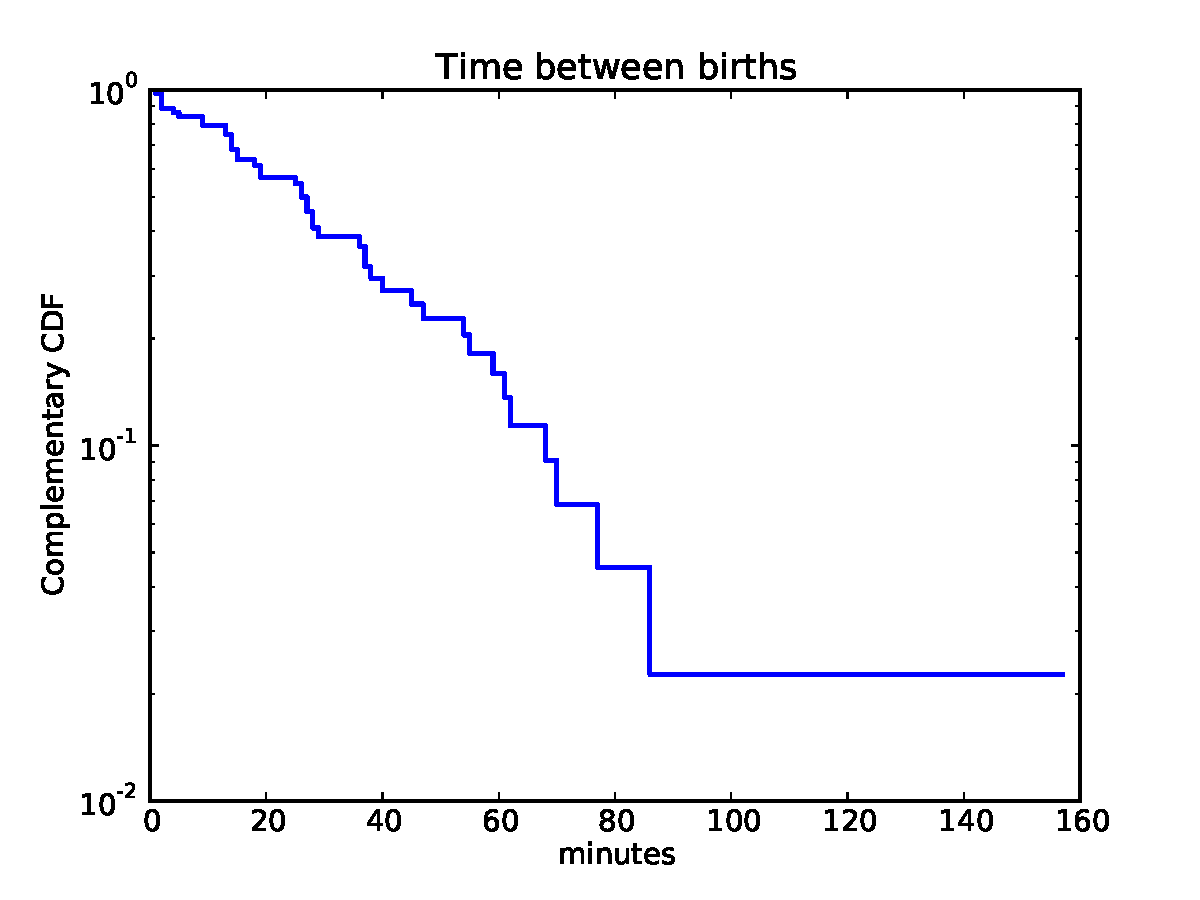
\includegraphics[height=2.5in]{figs/interarrivals_logy.pdf}}
\caption{CCDF of interarrival times.}
\label{interarrival_ccdf}
\end{figure}


\section{The Pareto distribution}
\index{Pareto distribution}
\index{distribution!Pareto}
\index{Pareto, Vilfredo}

The Pareto distribution is named after the economist Vilfredo Pareto,
who used it to describe the distribution of wealth (see
\url{http://wikipedia.org/wiki/Pareto_distribution}).  Since then, it has
been used to describe phenomena in the natural and social
sciences including sizes of cities and towns, sand particles and
meteorites, forest fires and earthquakes.
\index{CDF}

The CDF of the Pareto distribution is:
%
\[ CDF(x) = 1 - \left( \frac{x}{x_m} \right) ^{-\alpha} \]
%
The parameters $x_{m}$ and $\alpha$ determine the location and shape of
the distribution. $x_{m}$ is the minimum possible value.
Figure~\ref{pareto_cdf} shows the CDF of a Pareto distribution with
parameters $x_{m} = 0.5$ and $\alpha = 1$.
\index{parameter}

\begin{figure}
% continuous.py
\centerline{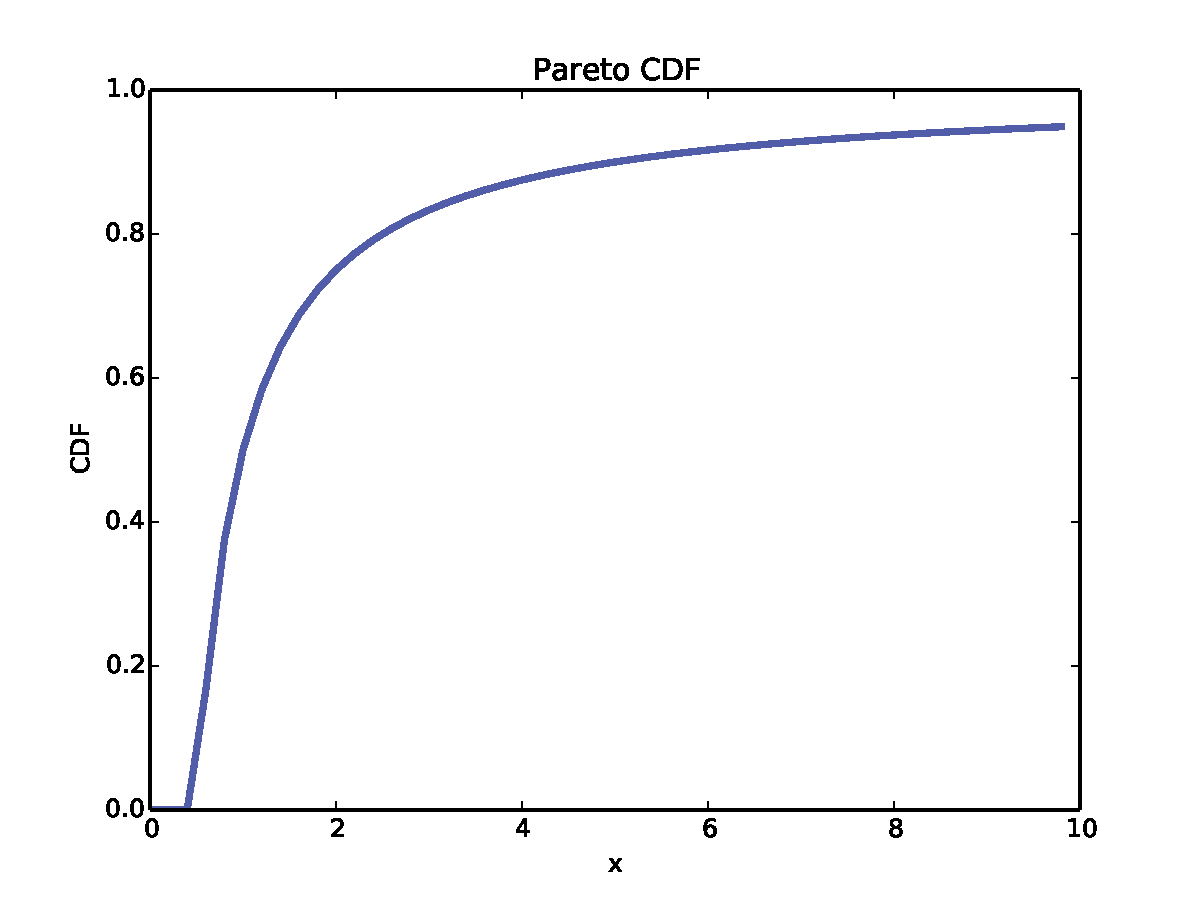
\includegraphics[height=2.5in]{figs/pareto_cdf.pdf}}
\caption{CDF of a Pareto distribution.}
\label{pareto_cdf}
\end{figure}

The median of a Pareto distribution is $x_m 2^{1/\alpha}$, so the
median of this distribution 1.  But the tail of the distribution is
skewed to the right; the 95th percentile is 10.  By contrast, the
exponential distribution with median 1 has 95th percentile of only
1.5.  \index{exponential distribution}
\index{distribution!exponential} \index{median} \index{logarithmic
  scale}

There is a simple visual test that indicates whether an empirical
distribution fits a Pareto distribution: on a log-log scale, the CCDF
looks like a straight line.
If you plot the CCDF of a sample from a Pareto distribution on a
linear scale, you expect to see a function like:
%
\[ y \approx \left( \frac{x}{x_m} \right) ^{-\alpha} \]
%
Taking the log of both sides yields:
%
\[ \log y \approx -\alpha (\log x - \log x_{m})\]
%
So if you plot $\log y$ versus $\log x$, it should look like a straight
line with slope $-\alpha$ and intercept
$\alpha \log x_{m}$.

\begin{exercise}
The {\tt random} module provides {\tt paretovariate},
which generates random values from a Pareto distribution.  It takes
a parameter for $\alpha$, but not $x_{m}$.  The
default value for $x_{m}$ is 1; you can generate a distribution
with a different parameter by multiplying by $x_{m}$.
\index{random module}
\index{Pareto distribution}
\index{distribution!Pareto}

Write a wrapper function named {\tt paretovariate} that takes
$\alpha$ and $x_{m}$ as parameters and uses {\tt
  random.paretovariate} to generate values from a two-parameter Pareto
distribution.
\index{parameter}

Use your function to generate a sample from a Pareto distribution.
Compute the CCDF and plot it on a log-log scale.  Is it a straight
line?  What is the slope?
\index{complementary CDF}
\index{CDF!complementary}
\index{CCDF}

\end{exercise}

\begin{exercise}
To get a feel for the Pareto distribution, imagine what the world
would be like if the distribution of human height were Pareto.
Choosing the parameters $x_{m} = 100$ cm and $\alpha = 1.7$, we
get a distribution with a reasonable minimum, 100 cm,
and median, 150 cm.
\index{height}

Generate 6 billion random values from this distribution.  What is the
mean of this sample?  What fraction of the population is shorter than
the mean?  How tall is the tallest person in Pareto World?
\index{Pareto World}

\end{exercise}

\begin{exercise}
Zipf's law is an observation about how often different words are used.
The most common words have very high frequencies, but there are many
unusual words, like ``hapaxlegomenon,'' that appear only a few times.
Zipf's law predicts that in a body of text, called a ``corpus,'' the
distribution of word frequencies is roughly Pareto.
\index{Pareto distribution}
\index{distribution!Pareto}
\index{Zipf's law}
\index{hapaxlegomenon}
\index{corpus}
\index{frequency}
\index{word frequency}

Find a large corpus, in any language, in electronic
format.  Count how many times each word appears.  Find the CCDF of the
word counts and plot it on a log-log scale.  Does Zipf's law hold?
What is the value of $\alpha$, approximately?
\index{complementary CDF}
\index{CDF!complementary}
\index{CCDF}

\end{exercise}

\begin{exercise}
\label{weibull}

The Weibull distribution is a generalization of the exponential
distribution that comes up in failure analysis
(see \url{http://wikipedia.org/wiki/Weibull_distribution}).  Its CDF is
%
\[ CDF(x) = 1 - e^{-(x / \lambda)^k} \]
%
Can you find a transformation that makes a Weibull distribution look
like a straight line?  What do the slope and intercept of the
line indicate?
\index{Weibull distribution}
\index{distribution!Weibull}
\index{exponential distribution}
\index{distribution!exponential}
\index{random module}

Use {\tt random.weibullvariate} to generate a sample from a
Weibull distribution and use it to test your transformation.

\end{exercise}


\section{The normal distribution}
\label{normal}
\index{normal distribution}
\index{distribution!normal}
\index{Gaussian distribution}
\index{distribution!Gaussian}

\newcommand{\erf}{\mathrm{erf}}

The normal distribution, also called Gaussian, is the most commonly
used because it describes so many phenomena, at least approximately.
It turns out that there is a good reason for its ubiquity, which we
will get to in Section~\ref{CLT}.
\index{error function}
\index{CDF}

The normal distribution has many properties that make it amenable for
analysis, but the CDF is not one of them.  Unlike the
other distributions we have looked at, there is no closed-form
expression for the normal CDF; the most common alternative is to write
it in terms of the {\bf error function}, which is a special function
written $\erf(x)$:
%
\[ CDF(x) = \frac{1}{2} \left[ 1 +
  \erf \left( \frac{x - \mu}{\sigma \sqrt{2}} \right) \right] \]
%
\[ \erf(x) = \frac{2}{\sqrt{\pi}} \int_{0}^x e^{-t^2} dt \]
%
The parameters $\mu$ and $\sigma$ determine the mean and standard
deviation of the distribution.
\index{parameter}
\index{{\tt erf.py}}

If these formulas make your eyes hurt, don't worry; they are easy to
implement in Python: {\tt erf} is available in the {\tt math} module,
and {\tt thinkstats2} provides {\tt GaussianCdf(x, mu=0, sigma=1)},
which evaluates a Gaussian CDF at $x$, with the given parameters.

Figure~\ref{normal_cdf} shows the CDF of the normal distribution
with parameters $\mu$ = 2.0 and $\sigma$ = 0.5.  The sigmoid shape of
this curve is a recognizable characteristic of a normal distribution.

\begin{figure}
% continuous.py
\centerline{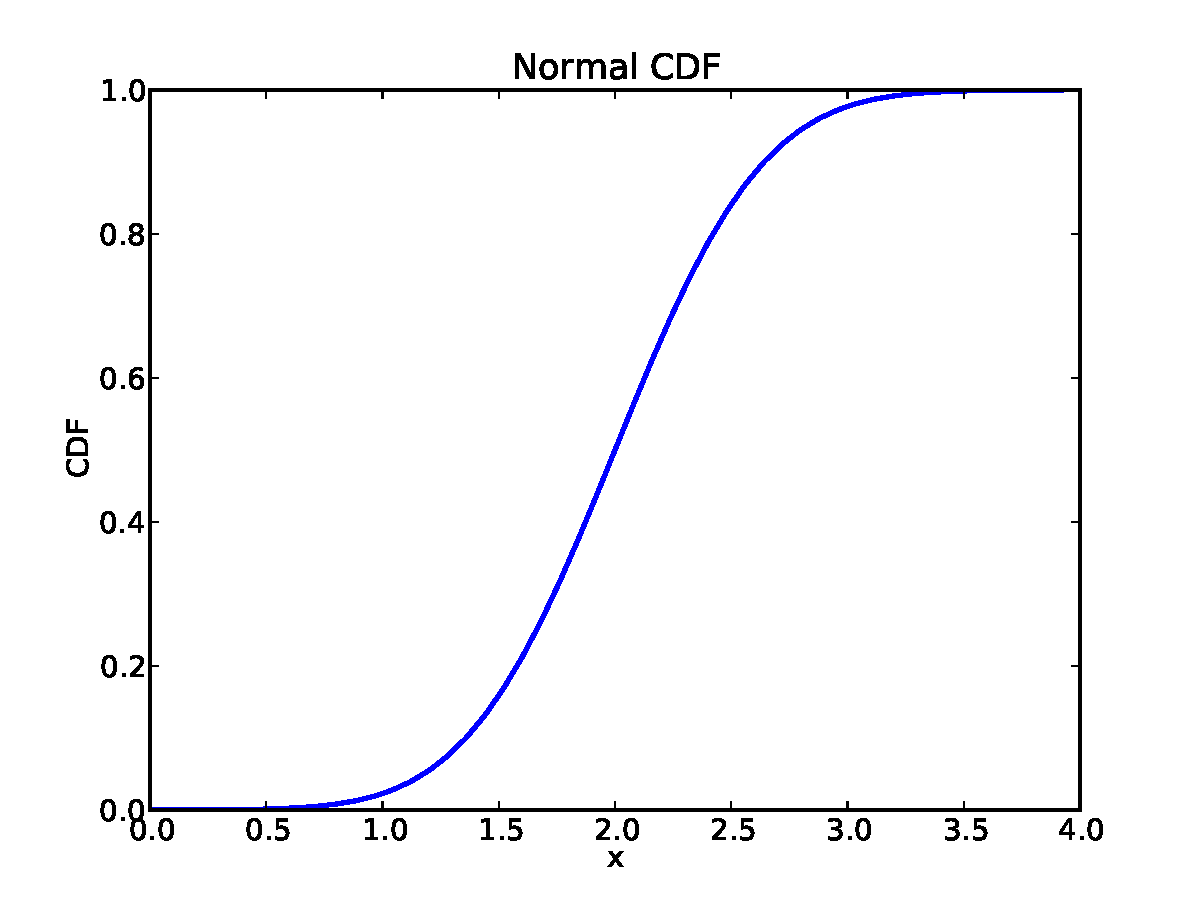
\includegraphics[height=2.5in]{figs/normal_cdf.pdf}}
\caption{CDF of a normal distribution.}
\label{normal_cdf}
\end{figure}

In the previous chapter we looked at the distribution of birth
weights in the NSFG.  Figure~\ref{nsfg_birthwgt_model} shows the
empirical CDF of weights for all live births and the CDF of
a normal distribution with the same mean and variance.
\index{National Survey of Family Growth}
\index{NSFG}
\index{birth weight}
\index{weight!birth}

\begin{figure}
% continuous.py
\centerline{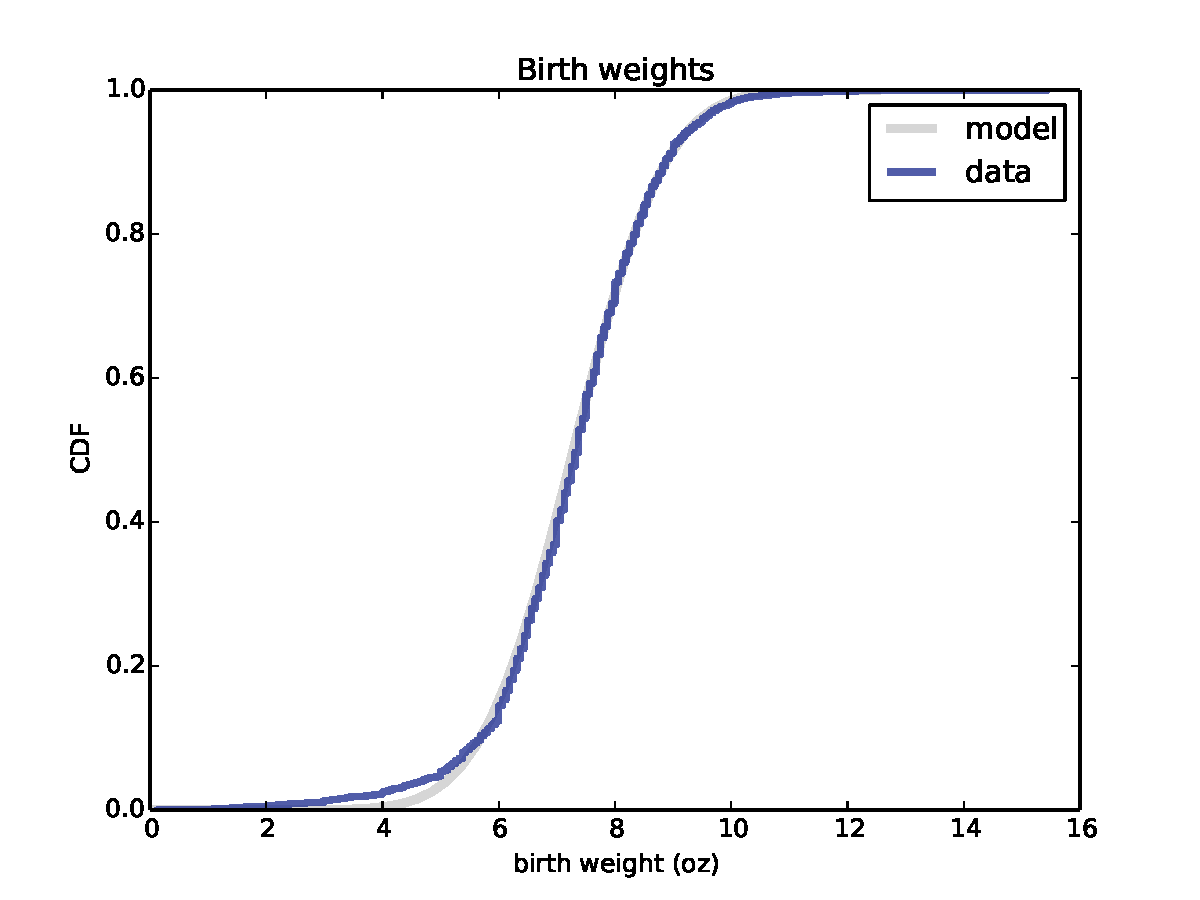
\includegraphics[height=2.5in]{figs/nsfg_birthwgt_model.pdf}}
\caption{CDF of birth weights with a normal model.}
\label{nsfg_birthwgt_model}
\end{figure}

The normal distribution is a good model for this dataset, so
we can summarize the distribution with the parameters
$\mu$ = 116.5 and $\sigma$ = 19.9, and the resulting error
(difference between the model and the data) is small.
\index{model}
\index{percentile}

Below the 10th percentile there is a discrepancy between the data
and the model; there are more light babies than we would expect in
a normal distribution.  If we are interested in studying preterm
babies, it would be important to get this part of the distribution
right, so it might not be appropriate to use the normal
model.

\begin{exercise}
In the BRFSS (see Section~\ref{lognormal}), the distribution of
heights is roughly normal with parameters $\mu$ = 178 cm and
$\sigma^2 = 59.4$ cm for men, and $\mu$ = 163 cm and $\sigma^2 = 52.8$ cm for
women.
\index{normal distribution}
\index{distribution!normal}
\index{height}
\index{Blue Man Group}
\index{Group, Blue Man}

In order to join Blue Man Group, you have to be male between 5'10''
and 6'1'' (see \url{http://bluemancasting.com}).  What percentage of the
U.S. male population is in this range?
\end{exercise}

\begin{exercise}
The Wechsler Adult Intelligence Scale is a test that is intended
to measure intelligence.\footnote{Whether it does or not is a
fascinating controversy that I invite you to investigate at your
leisure.}  Results are transformed so that the distribution of scores
in the general population is normal with $\mu$ = 100 and $\sigma$ = 15.
\index{Wechsler Adult Intelligence Scale}
\index{Adult Intelligence Scale}
\index{WAIS}
\index{IQ}
\index{intelligence}

Use {\tt thinkstats2.GaussianCdf} to investigate the frequency of rare
events in a normal distribution.  What fraction of the population has
an IQ greater than the mean?  What fraction is over 115?  130?  145?

A ``six-sigma'' event is a value that exceeds the mean by 6 standard
deviations, so a six-sigma IQ is 190.  In a world of 6 billion people,
how many do we expect to have an IQ of 190 or more?\footnote{On this
  topic, you might be interested to read
  \url{http://wikipedia.org/wiki/Christopher_Langan}.}
\index{Langan, Christopher}
\index{six-sigma event}

\end{exercise}


\begin{exercise}
Plot the CDF of pregnancy lengths for all live births.  Does it
look like a normal distribution?
\index{pregnancy length}
\index{length!pregnancy}

Compute the mean and standard deviation of the sample and plot the
normal distribution with the same parameters.  Is the normal
distribution a good model for this data?  If you had to summarize this
distribution with two statistics, what statistics would you choose?

\end{exercise}


\section{Normal probability plot}
\index{normal probability plot}
\index{plot!normal probability}
\index{exponential distribution}
\index{distribution!exponential}
\index{Weibull distribution}
\index{distribution!Weibull}
\index{Pareto distribution}
\index{distribution!Pareto}

For the exponential, Pareto and Weibull distributions, there are
simple transformations we can use to test whether a analytic
distribution is a good model of a dataset.
\index{model}
\index{normal distribution}
\index{distribution!normal}
\index{Gaussian distribution}
\index{distribution!Gaussian}

For the normal distribution there is no such transformation, but there
is an alternative called a {\bf normal probability plot}.  It is based
on {\bf rankits}: if you generate $n$ values from a normal
distribution and sort them, the $k$th rankit is the mean of the
distribution for the $k$th value.
\index{rankit}

\begin{exercise}
Write a function called {\tt Sample} that generates 6 samples from a
normal distribution with $\mu$ = 0 and $\sigma$ = 1.  Sort and return
the values.

Write a function called {\tt Samples} that calls {\tt Sample} 1000
times and returns a list of 1000 lists.

If you apply {\tt zip} to this list of lists, the result is 6 lists
with 1000 values in each.  Compute the mean of each of these lists
and print the results.  I predict that you will get something like
this:

\{-1.2672,   -0.6418,   -0.2016,   0.2016,   0.6418,   1.2672\}

If you increase the number of times you call {\tt Sample}, the
results should converge on these values.

\end{exercise}

% Algorithms for exact and approximate normal rank stats
% http://download.osgeo.org/grass/grass6_progman/as177_8c_source.html

Computing rankits exactly is moderately difficult, but there are
numerical methods for approximating them.

But you don't need rankits to generate a normal probability plot;
there is a quick-and-dirty method that is even easier to implement:

\begin{enumerate}

\item From a normal distribution with $\mu$ = 0 and $\sigma$ = 1,
generate a sample with the same size as your dataset and sort it.

\item Sort the values in the dataset.

\item Plot the sorted values from your dataset versus the random values.

\end{enumerate}

For large datasets, this method works well.
For smaller datasets, you can improve it by generating $m (n+1) - 1$
values from a normal distribution, where $n$ is the size of the
dataset and $m$ is a multiplier.  Then select every $m$th element,
starting with the $m$th.  

%Hint: use the Python slice operator.

This method works with other distributions as well, as long as
you know how to generate a random sample.

Figure~\ref{nsfg_birthwgt_normal} is a quick-and-dirty normal
probability plot for the birth weight data.
\index{birth weight}
\index{weight!birth}

\begin{figure}
% continuous.py
\centerline{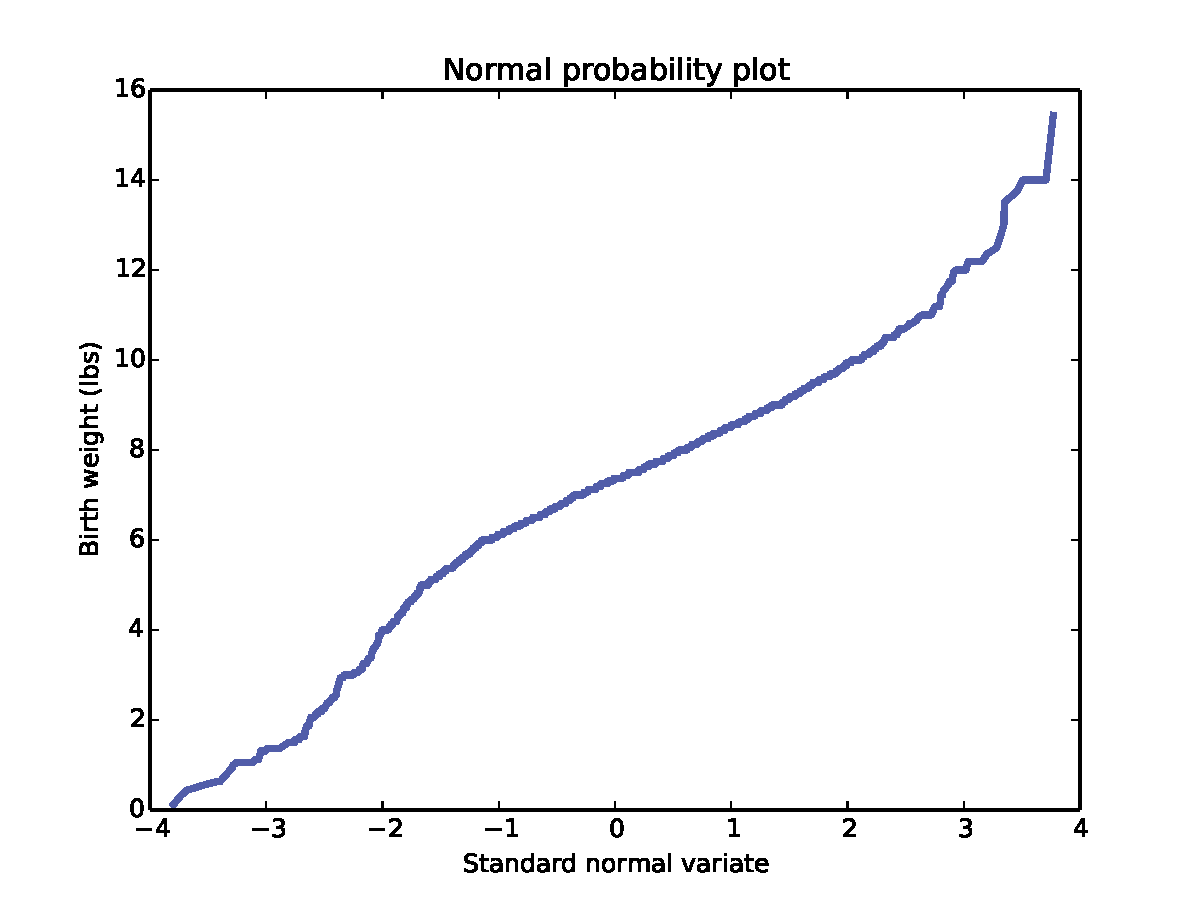
\includegraphics[height=2.5in]{figs/nsfg_birthwgt_normal.pdf}}
\caption{Normal probability plot of birth weights.}
\label{nsfg_birthwgt_normal}
\end{figure}

The curvature in this plot suggests that there are
deviations from a normal distribution; nevertheless, it is a
good (enough) model for many purposes.
\index{model}

% TODO: add a line to this plot and use the slope and intercept
% to estimate parameters

\begin{exercise}
Write a function called {\tt NormalPlot} that takes a sequence of
values and generates a normal probability plot.  You can download
a solution from \url{http://thinkstats2.com/rankit.py}.
\index{normal distribution}
\index{distribution!normal}
\index{Gaussian distribution}
\index{distribution!Gaussian}
\index{{\tt rankit.py}}
\index{{\tt relay.py}}
\index{{\tt relay\_normal.py}}
\index{relay race}
\index{race!relay}

Use the running speeds from {\tt relay.py} to generate a normal
probability plot.  Is the normal distribution a good model for this
data?  You can download a solution from
\url{http://thinkstats2.com/relay_normal.py}.

\end{exercise}


\section{The lognormal distribution}
\label{lognormal}
\index{lognormal distribution}
\index{distribution!lognormal}
\index{CDF}

If the logarithms of a set of values have a normal distribution, the
values have a {\bf lognormal} distribution.  The CDF of the lognormal
distribution is the same as the CDF of the normal distribution,
with $\log x$ substituted for $x$.
%
\[ CDF_{lognormal}(x) = CDF_{normal}(\log x)\]
%
The parameters of the lognormal distribution are usually denoted
$\mu$ and $\sigma$.  But remember that these parameters are {\em not}
the mean and standard deviation; the mean of a lognormal distribution
is $\exp(\mu +\sigma^2/2)$ and the standard deviation is
ugly (see \url{http://wikipedia.org/wiki/Log-normal_distribution}).
\index{parameter} \index{weight!adult} \index{adult weight}

It turns out that the distribution of weights for adults is
approximately lognormal.\footnote{I was tipped off to this possibility by a
  comment (without citation) at
  \url{http://mathworld.wolfram.com/LogNormalDistribution.html}.
  Subsequently I found a paper that proposes the log transform and
  suggests a cause: Penman and Johnson, ``The Changing Shape of the
  Body Mass Index Distribution Curve in the Population,'' Preventing
  Chronic Disease, 2006 July; 3(3): A74.  Online
  at \url{http://www.ncbi.nlm.nih.gov/pmc/articles/PMC1636707}.}

The National Center for Chronic Disease
Prevention and Health Promotion conducts an annual survey as part of
the Behavioral Risk Factor Surveillance System
(BRFSS).\footnote{Centers for Disease Control and Prevention
  (CDC). Behavioral Risk Factor Surveillance System Survey
  Data. Atlanta, Georgia: U.S. Department of Health and Human
  Services, Centers for Disease Control and Prevention, 2008.}  In
2008, they interviewed 414,509 respondents and asked about their
demographics, health and health risks.
\index{Behavioral Risk Factor Surveillance System}
\index{BRFSS}


\begin{figure}
% cumulative.py
\centerline{
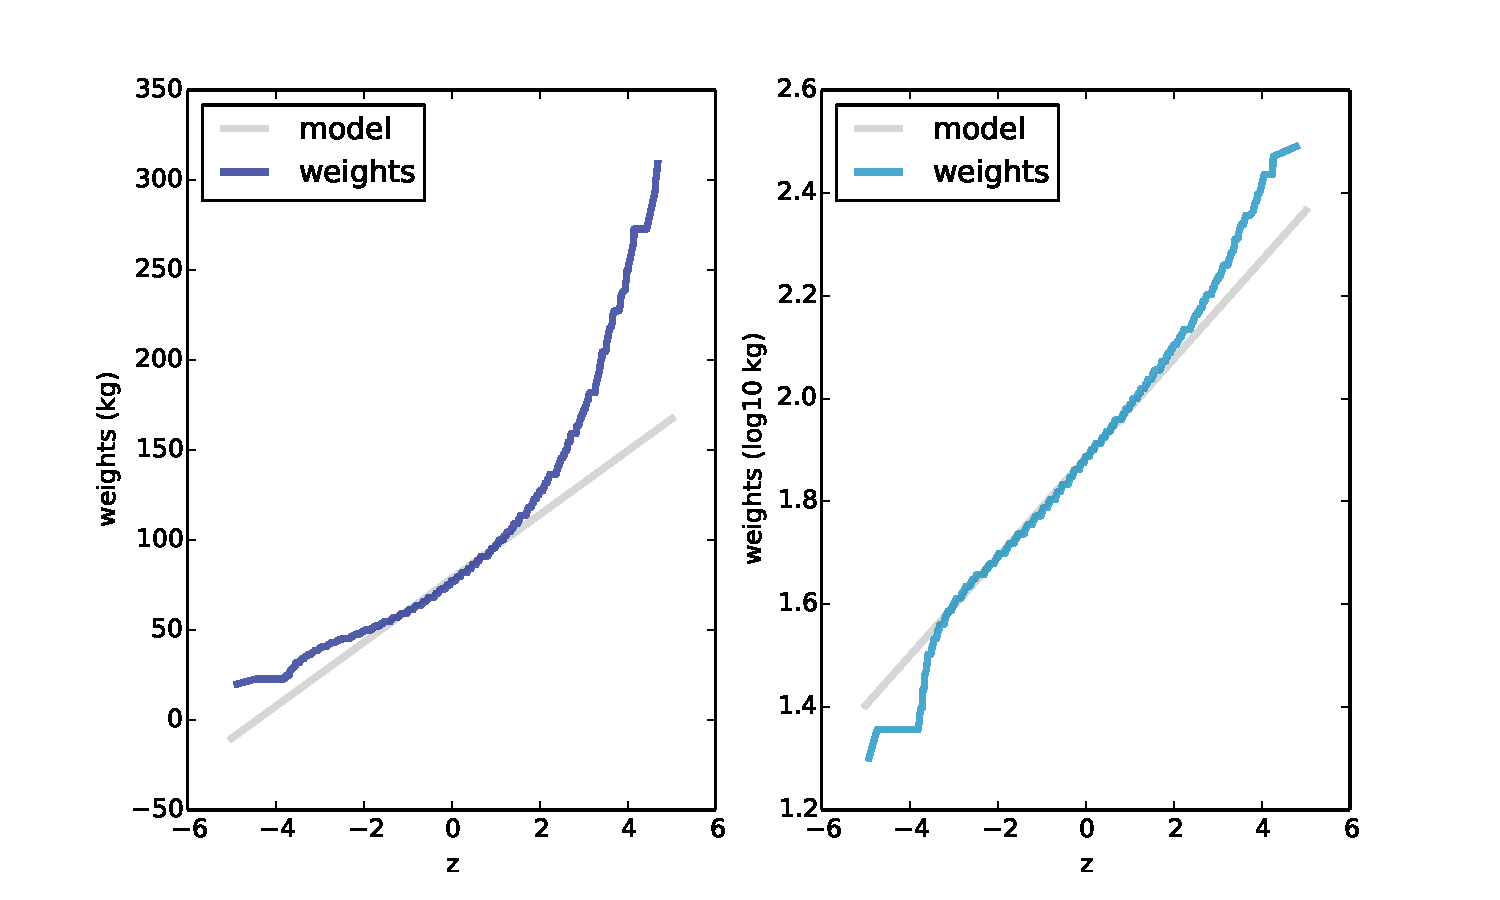
\includegraphics[height=2.5in]{figs/brfss_weight_log.pdf}
}
\caption{CDF of adult weights (log
  transform).}
\label{brfss_weight_log}
\end{figure}

Among the data they collected are the weights in kilograms of
398,484 respondents.
Figure~\ref{brfss_weight_log} shows the distribution
of $\log w$, where $w$ is weight in kilograms, along with a normal
model.
\index{respondent}
\index{model}

The normal model is a good fit for the data, although the highest
weights exceed what we expect from the normal model even after the log
transform.  Since the distribution of $\log w$ fits a normal
distribution, we conclude that $w$ fits a lognormal distribution.
\index{normal distribution} \index{distribution!normal}
\index{Gaussian distribution} \index{distribution!Gaussian}
\index{lognormal distribution} \index{distribution!lognormal}


%Figure~\ref{brfss_weight_model} shows the
%distribution of these weights and a normal model with the same mean
%and variance.

%\begin{figure}
%\centerline{\includegraphics[height=2.5in]{figs/brfss_weight_model.pdf}}
%\caption{CDF of adult weights from the BRFSS.}
%\label{brfss_weight_model}
%\end{figure}

%The agreement between the data and the model might be good enough
%for some purposes, but there are clear discrepancies below the 10th
%and above the 90th percentile.

%\begin{figure}
%\centerline{
%\begin{tabular}{cc}
%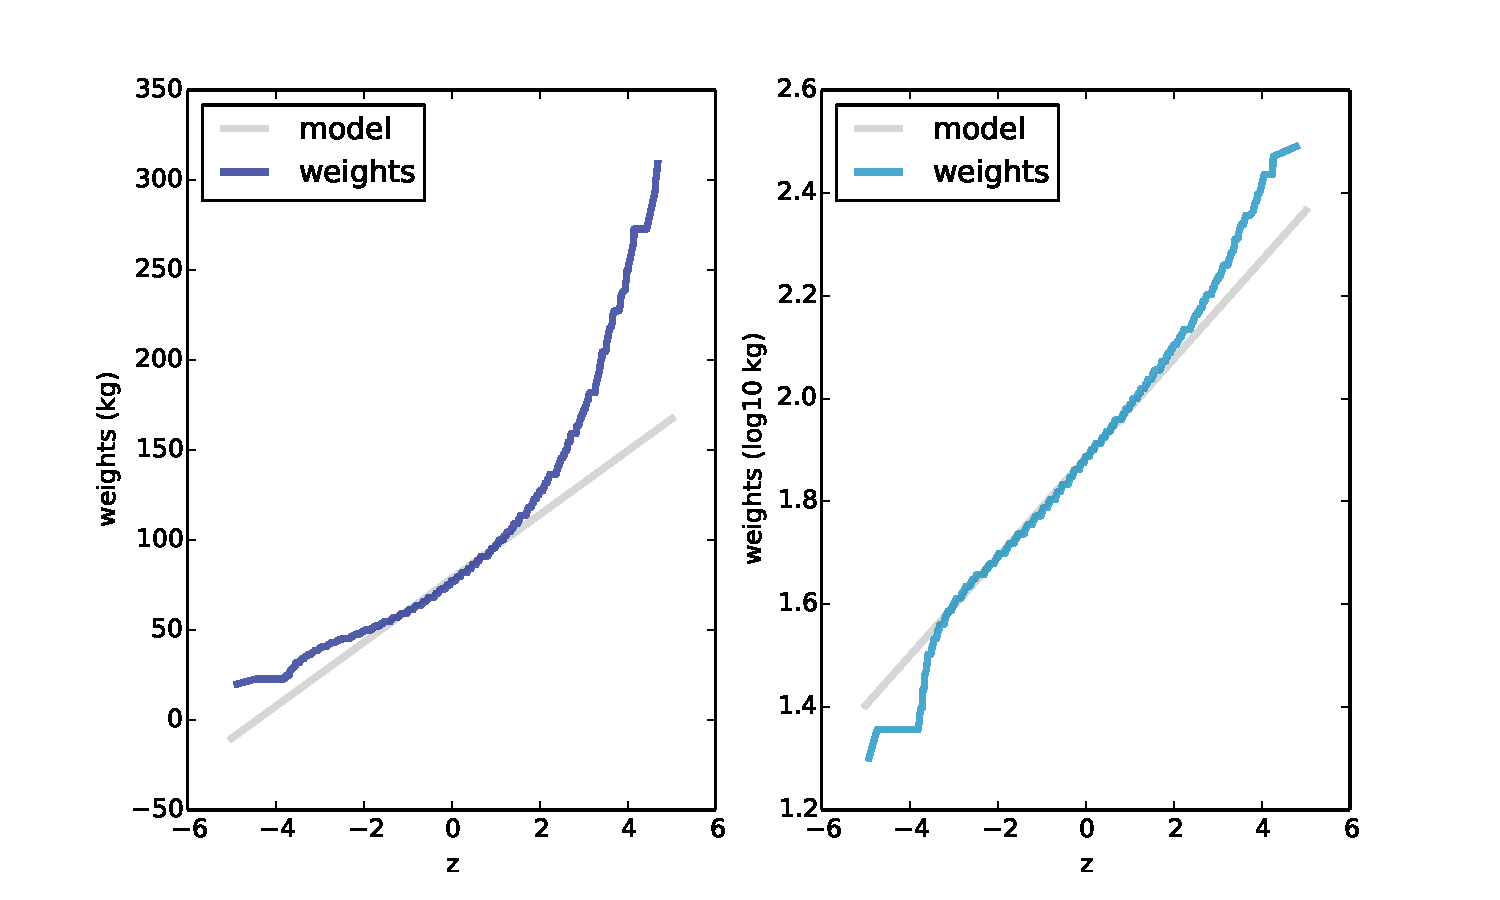
\includegraphics[height=2.3in]{figs/brfss_weight_log.pdf}
%\includegraphics[height=2.3in]{figs/brfss_weight_lognormal.pdf}
%\end{tabular}
%}
%\caption{CDF and normal probability plot for adult weights (log
%  transform).}
%\label{brfss_weight_log}
%\end{figure}

\begin{exercise}
Download the BRFSS data from 
\url{http://thinkstats2.com/CDBRFS08.ASC.gz}, and my code for reading it
from
\url{http://thinkstats2.com/brfss.py}.  Run {\tt brfss.py} and confirm that
it prints summary statistics for a few of the variables.
\index{Behavioral Risk Factor Surveillance System}
\index{BRFSS}
\index{{\tt brfss.py}}
\index{{\tt brfss\_figs.py}}
\index{weight!adult}
\index{adult weight}

Write a program that reads adult weights from the BRFSS and
generates normal probability plots for $w$ and $\log w$.  You can
download a solution from \url{http://thinkstats2.com/brfss_figs.py}.

\end{exercise}

\begin{exercise}
The distribution of populations for cities and towns has been proposed
as an example of a real-world phenomenon that can be described
with a Pareto distribution.
\index{Pareto distribution}
\index{distribution!Pareto}
\index{U.S.~Census Bureau}
\index{population}
\index{city size}

The U.S.~Census Bureau publishes data on the population of every
incorporated city and town in the United States.  I have written a
small program that downloads this data and stores it in a file.  You
can download it from \url{http://thinkstats2.com/populations.py}.
\index{{\tt populations.py}}

\begin{enumerate}

\item Read over the program to make sure you know what it does; then
  run it to download and process the data.

\item Write a program that computes and plots the distribution of
  populations for the 14,593 cities and towns in the dataset.

\item Plot the CDF on linear and log-x scales so you can get a sense
  of the shape of the distribution.  Then plot the CCDF on a log-log
  scale to see if it has the characteristic shape of a Pareto
  distribution.
\index{complementary CDF}
\index{CDF!complementary}
\index{CCDF}

\item Try out the other transformations and plots in this chapter to
  see if there is a better model for this data.

\end{enumerate}

What conclusion do you draw about the distribution of sizes
for cities and towns?  You can download a solution from
\url{http://thinkstats2.com/populations_cdf.py}.
\index{{\tt populations\_cdf.py}}

\end{exercise}


\begin{exercise}
\label{irs}

The Internal Revenue Service of the United States (IRS) provides data
about income taxes at \url{http://irs.gov/taxstats}.
\index{Internal Revenue Service}
\index{IRS}
\index{income}
\index{taxes}

One of their files, containing information about individual incomes
for 2008, is available from \url{http://thinkstats2.com/08in11si.csv}.  I
converted it to a text format called CSV, which stands for
``comma-separated values;'' you can read it using the {\tt csv}
module.

Extract the distribution of incomes from this dataset.  Are any of
the analytic distributions in this chapter a good model of
the data?  You can download a solution from \url{http://thinkstats2.com/irs.py}.
\index{{\tt irs.py}}

\end{exercise}


\section{Why model?}
\index{model}

At the beginning of this chapter I said that many real world phenomena
can be modeled with analytic distributions.  ``So,'' you might ask,
``what?''
\index{abstraction}

Like all models, analytic distributions are abstractions, which
means they leave out details that are considered irrelevant.
For example, an observed distribution might have measurement errors
or quirks that are specific to the sample; analytic models smooth
out these idiosyncrasies.
\index{smoothing}

Analytic models are also a form of data compression.  When a model
fits a dataset well, a small set of parameters can summarize a
large amount of data.
\index{parameter}
\index{compression}

It is sometimes surprising when data from a natural phenomenon fit a
analytic distribution, but these observations can lead to insight
into physical systems.  Sometimes we can explain why an observed
distribution has a particular form.  For example, Pareto distributions
are often the result of generative processes with positive feedback
(so-called preferential attachment processes: see
\url{http://wikipedia.org/wiki/Preferential_attachment}.).
\index{preferential attachment}
\index{generative process}
\index{Pareto distribution}
\index{distribution!Pareto}
\index{analysis}

Finally, analytic distributions lend themselves to mathematical
analysis, as we will see in Chapter~\ref{operations}.


\section{Generating random numbers}
\index{exponential distribution}
\index{distribution!exponential}
\index{random number}
\index{CDF}
\index{inverse CDF algorithm}
\index{uniform distribution}
\index{distribution!uniform}

Analytic CDFs are also useful for generating random numbers.
If there is an efficient way to compute the inverse CDF, $ICDF(p)$,
we can generate random values with the appropriate distribution
by choosing from a uniform distribution from 0 to 1, then choosing
%
\[ x = ICDF(p)\]
%
For example, the CDF of the exponential distribution is
%
\[ p = 1 - e^{-\lambda x} \]
%
Solving for $x$ yields:
%
\[ x = -\log (1 - p) / \lambda \]
%
So in Python we can write
%
\begin{verbatim}
def expovariate(lam):
    p = random.random()
    x = -math.log(1-p) / lam
    return x
\end{verbatim}

I called the parameter \verb"lam" because \verb"lambda" is a Python
keyword.  Most implementations of {\tt random.random} can return 0 but
not 1, so $1 - p$ can be 1 but not 0, which is good, because $\log 0$ is
undefined.
\index{random module}

\begin{exercise}
Write a function named \verb"weibullvariate" that takes
\verb"lam" and \verb"k" and returns a random value from the Weibull
distribution with those parameters.
\index{Weibull distribution}
\index{distribution!Weibull}
\index{parameter}

\end{exercise}


\section{Glossary}

\begin{itemize}

\item empirical distribution: The distribution of values in a sample.
\index{empirical distribution}
\index{distribution!empirical}

\item analytic distribution: A distribution described by a analytic
function.
\index{analytic distribution}
\index{distribution!analytic}

\item interarrival time: The elapsed time between two events.
\index{interarrival time}

\item error function: A special mathematical function, so-named
  because it comes up in the study of measurement errors.
\index{error function}

\item normal probability plot: A plot of the sorted values in a sample
versus the expected value for each if their distribution is normal.
\index{normal probability plot}
\index{plot!normal probability}

\item rankit: The expected value of an element in a sorted list of
values from a normal distribution.
\index{rankit}

\item model: A useful simplification.  Analytic distributions are
often good models of more complex empirical distributions.
\index{model}

\item corpus: A body of text used as a sample of a language.
\index{corpus}

\item hapaxlegomenon: A word that appears only once in a corpus.
It appears twice in this book, so far.
\index{hapaxlegomenon}

\end{itemize}


\chapter{Probability Density}

\section{PDFs}
\label{density}
\index{PDF}
\index{probability density function}
\index{exponential distribution}
\index{distribution!exponential}
\index{normal distribution}
\index{distribution!normal}
\index{Gaussian distribution}
\index{distribution!Gaussian}
\index{CDF}
\index{derivative}

The derivative of a CDF is called a {\bf probability density function},
or PDF.  For example, the PDF of an exponential distribution is
%
\[ \PDF_{expo}(x) = \lambda e^{-\lambda x}   \]
%
The PDF of a normal distribution is
%
\[ \PDF_{normal}(x) = \frac{1}{\sigma \sqrt{2 \pi}} 
                 \exp \left[ -\frac{1}{2} 
                 \left( \frac{x - \mu}{\sigma} \right)^2 \right]  \]
%
Evaluating a PDF for a particular value of $x$ is usually not useful.
The result is not a probability; it is a probability {\em density}.
\index{density}
\index{mass}

In physics, density is mass per unit of
volume; in order to get a mass, you have to multiply by volume or,
if the density is not constant, you have to integrate over volume.

Similarly, probability density measures probability per unit of $x$.
In order to get a probability mass, you have to integrate over $x$.

{\tt thinkstats2} provides a class called {\tt Pdf} that represents
a probability density function.  Every Pdf object provides the
following methods:

\begin{itemize}

\item {\tt Density}, which takes a value, {\tt x}, and returns the
  density of the distribution at {\tt x}.

\item {\tt MakePmf}, which evaluates the density at a discrete set of
  values and returns a Pmf that approximates the Pdf.  The parameter
  of {\tt MakePmf} is a sequence of {\tt x} values.

\end{itemize}  

{\tt Pdf} is an abstract parent class, which means you should not
instantiate it; that is, you cannot create a Pdf object.
Instead, you should define a child class that inherits from {\tt Pdf}
and provides the appropriate definition of {\tt Density}.  For
example, {\tt thinkstats2} provides a class named {\tt GaussianPdf}
that evaluates the Gaussian density function.

The following example creates a GaussianPdf with the mean and variance
of adult female heights, in cm, from the BRFSS.  Then it computes the
density of the distribution at a location one standard deviation from
the mean.

\begin{verbatim}
    mean, var = 163, 52.8
    sigma = math.sqrt(var)
    pdf = thinkstats2.GaussianPdf(mean, sigma)
    print pdf.Density(mean + sigma)
\end{verbatim}

The result is about 0.09, in units of probability mass per cm.
Again, a probability density doesn't mean much by itself.  But if
we make a Pmf, we can plot it and see the shape of the distribution:

\begin{verbatim}
    xs = numpy.linspace(mean - 3*sigma, mean + 3*sigma, 100)
    pmf = pdf.MakePmf(xs)
    thinkplot.Pmf(pmf, label='Gaussian')
\end{verbatim}

{\tt numpy.linspace} returns a Numpy array with 100 values, equally
spaced from three standard deviations below the mean to three standard
deviations above.

\begin{figure}
% pdf_example.py
\centerline{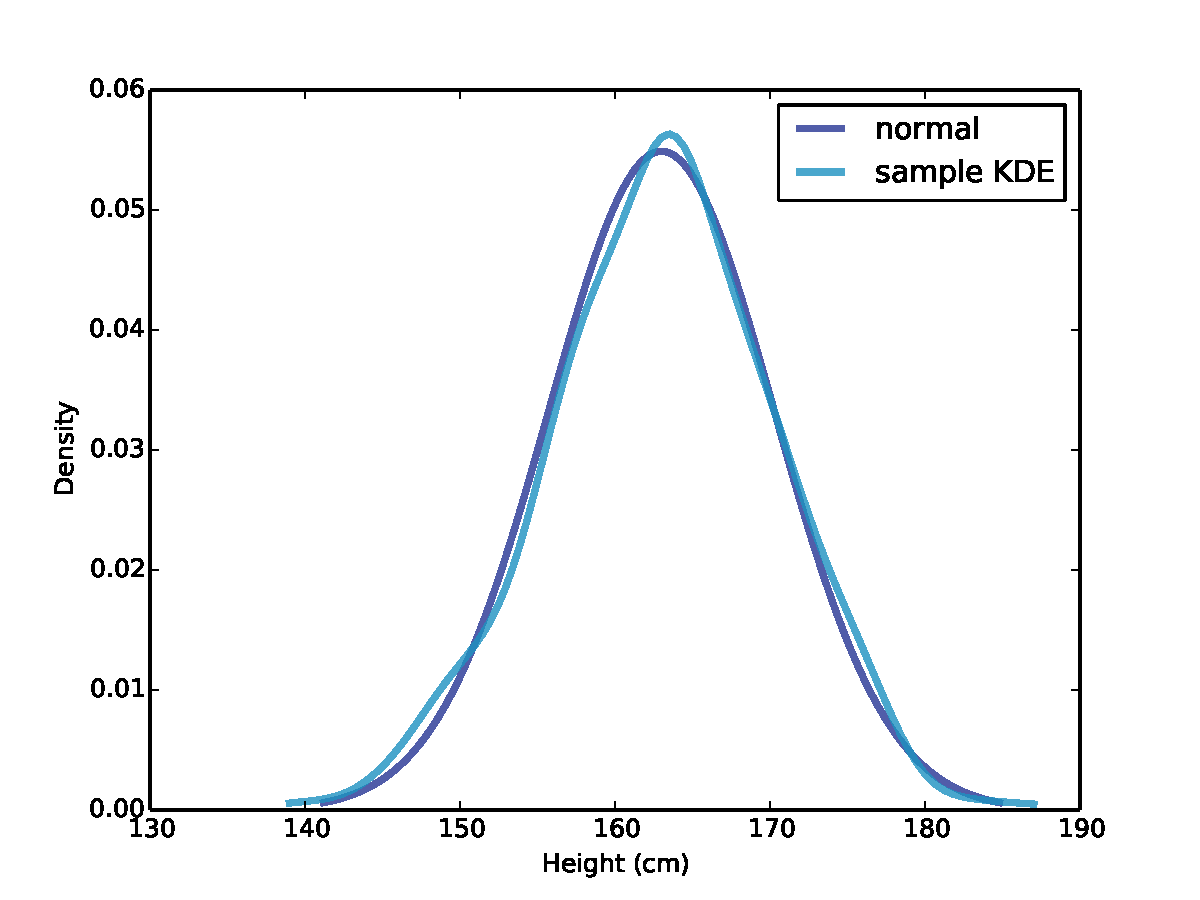
\includegraphics[height=2.2in]{figs/pdf_example.pdf}}
\caption{A Gaussian PDF that models adult human height in the U.S.,
and the kernel density estimate of a sample with $n=1000$.}
\label{pdf_example}
\end{figure}


\section{Kernel density estimation} 

Kernel density estimation (KDE) is an algorithm that takes
a sample and finds an appropriately smooth PDF that fits 
the data.  You can read details at
\url{http://en.wikipedia.org/wiki/Kernel_density_estimation}.
\index{KDE}
\index{kernel density estimation}

{\tt scipy} provides an implementation of KDE and {\tt thinkstats2}
provides a class called {\tt EstimatedPdf} that uses it:
\index{scipy}
\index{numpy}

\begin{verbatim}
class EstimatedPdf(Pdf):

    def __init__(self, sample):
        self.kde = scipy.stats.gaussian_kde(sample)

    def Density(self, x):
        return self.kde.evaluate(x)
\end{verbatim}

\verb"__init__" takes a sample
and computes a kernel density estimate.  The result is a
\verb"gaussian_kde" object that provides an {\tt evaluate}
method.

{\tt Density} takes a value, calls \verb"gaussian_kde.evaluate",
and returns the resulting density.
\index{density}

Here's an example that generates a sample from a Gaussian
distribution and generates an EstimatedPdf to fit it:
\index{numpy}

\begin{verbatim}
    sample = [random.gauss(mean, sigma) for i in range(1000)]
    sample_pdf = thinkstats2.EstimatedPdf(sample)
    sample_pmf = sample_pdf.MakePmf(xs)
    thinkplot.Pmf(pmf, label='KDE')
\end{verbatim}

\verb"sample" is a list of 1000 random heights.
\verb"sample_pdf" is a {\tt Pdf} object that containts the estimated
KDE of the sample.  {\tt pmf} is a Pmf object that approximates the Pdf by
evaluating the density at a sequence of equally spaced values.

Figure~\ref{pdf_example} shows the Gaussian density function (actually
a discrete approximation of it) and a KDE based on a sample of 1000
random heights.  The estimate is a good match for the original
distribution.



\section{Random Variables}
\index{random variable}
\index{variable!random}

A {\bf random variable} represents a process that generates a random
number.  Random variables are usually written with a capital letter,
like $X$.  You can think of a random variable as a random number
generator.
\index{cumulative distribution function}
\index{CDF}

For example, here is a definition for a class that represents
random variables:
%
\begin{verbatim}
class RandomVariable(object):
    """Parent class for all random variables."""
\end{verbatim}

And here is a random variable with an exponential distribution:
\index{exponential distribution}
\index{distribution!exponential}
%
\begin{verbatim}
class Exponential(RandomVariable):
    def __init__(self, lam):
        self.lam = lam

    def Generate(self):
        return random.expovariate(self.lam)
\end{verbatim}

The \verb"__init__" method takes the parameter, $\lambda$, and stores it as
an attribute.  The {\tt Generate} method returns a random value
from the exponential distribution with that parameter.
\index{init method}
\index{method!init}

Each time you invoke {\tt Generate}, you get a different value.  The
value you get is called a {\bf random variate}, which is why many
function names in the {\tt random} module include the word ``variate.''
\index{random variate}
\index{variate!random}

If I were just generating exponential variates, I would not bother to
define a new class; I would use {\tt random.expovariate}.  But for
other distributions it might be useful to use RandomVariable objects.
For example, the Erlang distribution is a continuous distribution with
parameters $\lambda$ and $k$ (see
\url{http://wikipedia.org/wiki/Erlang_distribution}).
\index{Erlang distribution}
\index{distribution!Erlang}

One way to generate values from an Erlang distribution is to add
$k$ values from an exponential distribution with the same $\lambda$.
Here's an implementation:
%
\begin{verbatim}
class Erlang(RandomVariable):
    def __init__(self, lam, k):
        self.lam = lam
        self.k = k
        self.expo = Exponential(lam)

    def Generate(self):
        total = 0
        for i in range(self.k):
            total += self.expo.Generate()
        return total
\end{verbatim}

The \verb"__init__" method creates an Exponential object with the
given parameter; then {\tt Generate} uses it.  In general,
\verb"__init__" can take any set of parameters and the {\tt
  Generate} function can implement any random process.

\begin{exercise}
Write a definition for a class that represents a random variable
with a Gumbel distribution (see \url{http://wikipedia.org/wiki/Gumbel_distribution}).
\index{Gumbel distribution}
\index{distribution!Gumbel}

\end{exercise}


\section{Functions of random variables}
\index{random variables}
\index{CDF}

Suppose we have two random variables, $X$ and $Y$, represented
by RandomVariable objects.
How can we compute the distribution of the sum $Z = X + Y$?
\index{random variable}
\index{variable!random}
\index{sum}

One option is to write a RandomVariable object that generates
the sum:
%
\begin{verbatim}
class Sum(RandomVariable):
    def __init__(X, Y):
        self.X = X
        self.Y = Y

    def Generate():
        return X.Generate() + Y.Generate()
\end{verbatim}

Given any RandomVariables, $X$ and $Y$, we can create a Sum
object that represents $Z$.  Then we can use a sample from $Z$ to
approximate $\CDF_{Z}$.

This approach is simple and versatile, but not very efficient; we
have to generate a large sample to estimate $\CDF_{Z}$ accurately, and
even then it is not exact.


\begin{exercise}
Suppose I draw two values from a distribution; what is the distribution
of the larger value?  Write a RandomVariable class called {\tt Max}
that generates values from $Z = max(X, Y)$.
\index{max}

As the number of values increases, the distribution of the maximum
converges on one of the extreme value distributions; see
\url{http://wikipedia.org/wiki/Gumbel_distribution}.
\index{Gumbel distribution}
\index{distribution!Gumbel}

\end{exercise}

\begin{exercise}
If you are given Pmf objects, you can compute the distribution of
the sum by enumerating all pairs of values:
\index{Pmf object}
%
\begin{verbatim}
for x in pmf_x.Values():
    for y in pmf_y.Values():
        z = x + y
\end{verbatim}

Write a function that takes $PMF_{X}$ and
$PMF_{Y}$ and returns a new Pmf that represents the distribution of
the sum $Z = X + Y$.

Write a similar function that computes the PMF of $Z = max(X, Y)$.

\end{exercise}



\section{Why normal?}
\label{why_normal}
\index{normal distribution}
\index{distribution!normal}
\index{Gaussian distribution}
\index{distribution!Gaussian}

I said earlier that normal distributions are amenable to analysis,
but I didn't say why.  One reason is that they are
closed under linear transformation and convolution.  To explain what
that means, it will help to introduce some notation.
\index{analysis}
\index{random variable}
\index{variable!random}

If the distribution of a random variable, X, is
normal with parameters $\mu$ and $\sigma$, you can write
%
\[ X \sim \normal (\mu, \sigma^{2})\]
%
where the symbol $\sim$ means ``is distributed'' and the script letter
$\normal$ stands for ``normal.''

%The other continuous distributions in this chapter are sometimes
%written $\mathrm{Exponential}(\lambda)$, $\mathrm{Pareto}(x_m,
%\alpha)$ and, for lognormal, $\mathrm{Log}-\normal (\mu,
%\sigma^2)$.

A linear transformation of $X$ is something like $X' = a X + b$, where
$a$ and $b$ are real numbers.\index{linear transformation}
A family of distributions is closed under
linear transformation if $X'$ is in the same family as $X$.  The normal
distribution has this property; if $X \sim \normal (\mu,
\sigma^2)$,

\[ X' \sim \normal (a \mu + b, a^{2} \sigma^2)\]

Normal distributions are also closed under addition.  
If $Z = X + Y$ and
$X \sim \normal (\mu_{X}, \sigma_{X}^{2})$ and
$Y \sim \normal (\mu_{Y}, \sigma_{Y}^{2})$ then
%
\[ Z \sim \normal (\mu_X + \mu_Y, \sigma_X^2 + \sigma_Y^2) \]
%
The other distributions we have looked at do not have these
properties.
\index{convolution}

\begin{exercise}
If 
$X \sim \normal (\mu_{X}, \sigma_{X}^{2})$ and
$Y \sim \normal (\mu_{Y}, \sigma_{Y}^{2})$, what 
is the distribution of Z = aX + bY?

\end{exercise}

\begin{exercise}
Let's see what happens when we add values from
other distributions.  Choose a pair of distributions (any two of
exponential, normal, lognormal, and Pareto) and choose parameters
that make their mean and variance similar.
\index{exponential distribution}
\index{distribution!exponential}
\index{Pareto distribution}
\index{distribution!Pareto}
\index{lognormal distribution}
\index{distribution!lognormal}
\index{sum}

Generate random numbers from these distributions and compute the
distribution of their sums.  Use the tests from
Chapter~\ref{continuous} to see if the sum can be modeled by a
continuous distribution.

\end{exercise}



\section{Central limit theorem}
\label{CLT}
\index{Central Limit Theorem}

So far we have seen:

\begin{itemize}

\item If we add values drawn from normal distributions, the distribution
of the sum is normal.
\index{sum}
\index{normal distribution}
\index{distribution!normal}
\index{Gaussian distribution}
\index{distribution!Gaussian}

\item If we add values drawn from other distributions, the sum does not
generally have one of the continuous distributions we have seen.

\end{itemize}

But it turns out that if we add up a large number of values from
almost any distribution, the distribution of the sum converges to
normal.

More specifically, if the distribution of the values has mean and
standard deviation $\mu$ and $\sigma$, the distribution of the sum is
approximately $\normal(n \mu, n \sigma^2)$.

This is called the {\bf Central Limit Theorem}.  It is one of the
most useful tools for statistical analysis, but it comes with
caveats:

\begin{itemize}

\item The values have to be drawn independently.
\index{independent}

\item The values have to come from the same distribution (although
  this requirement can be relaxed).
\index{identical}

\item The values have to be drawn
  from a distribution with finite mean and variance, so most Pareto
  distributions are out.
\index{mean}
\index{variance}
\index{Pareto distribution}
\index{distribution!Pareto}
\index{exponential distribution}
\index{distribution!exponential}

\item The number of values you need before you see convergence depends
  on the skewness of the distribution.  Sums from an exponential
  distribution converge for small sample sizes.  Sums from a
  lognormal distribution do not.
\index{lognormal distribution}
\index{distribution!lognormal}

\end{itemize}

The Central Limit Theorem explains, at least in part, the prevalence
of normal distributions in the natural world.  Most characteristics of
animals and other life forms are affected by a large number of genetic
and environmental factors whose effect is additive.  The characteristics
we measure are the sum of a large number of small effects, so their
distribution tends to be normal.
\index{normal distribution}
\index{distribution!normal}
\index{Gaussian distribution}
\index{distribution!Gaussian}

\begin{exercise}
If I draw a sample, $x_{1} .. x_{n}$, independently from a
distribution with finite mean $\mu$ and variance $\sigma^2$, what is
the distribution of the sample mean:
%
\[ \xbar = \frac{1}{n} \sum x_i \]
%
As $n$ increases, what happens to the variance of the sample mean?
Hint: review Section~\ref{why_normal}.

\end{exercise}

\begin{exercise}
Choose a distribution (one of exponential, lognormal or Pareto) and
choose values for the parameter(s).  Generate samples with sizes
2, 4, 8, etc., and compute the distribution of their sums.  Use
a normal probability plot to see if the distribution is approximately
normal.  How many terms do you have to add to see convergence?
\index{exponential distribution}
\index{distribution!exponential}
\index{Pareto distribution}
\index{distribution!Pareto}
\index{lognormal distribution}
\index{distribution!lognormal}
\index{convergence}

\end{exercise}


\begin{exercise}
Instead of the distribution of sums, compute the distribution of
products; what happens as the number of terms increases?
Hint: look at the distribution of the log of the products.
\index{logarithm}
\index{product}

\end{exercise}


\section{Moments}
\index{moment}

Any time you take a sample and reduce it to a single number, that
number is a statistic.  The statistics we have seen so far include
mean, variance, median, and interquartile range.

A {\bf raw moment} is a kind of statistic.  If you have a sample of
values, $x_i$, the $k$th raw moment is:
%
\[ m'_k = \frac{1}{n} \sum_i x_i^k \]
%
Or if you prefer Python notation:

\begin{verbatim}
def RawMoment(xs, k):
    return sum(x**k for x in xs) / float(len(xs))
\end{verbatim}

When $k=1$ the result is the sample mean, $\xbar$.  The other
raw moments don't mean much by themselves, but they are used
in some computations.

Some of the {\bf central moments} are more useful.  The
$k$th central moment is:
%
\[ m_k = \frac{1}{n} \sum_i (x_i - \xbar)^k \]
%
Or in Python:

\begin{verbatim}
def CentralMoment(xs, k):
    xbar = RawMoment(xs, 1)
    return sum((x - xbar)**k for x in xs) / len(xs)
\end{verbatim}

When $k=2$ the result is the second central moment, also known
as the variance.  The definition of variance gives a hint about
why these statistics are called moments.  If we place a mass
along a number line at each value, $x_i$, and then spin the
number line around the mean, the moment of inertia of the spinning
masses is the variance of the values.
\index{moment of intertia}.

When you report moment-based statistics, it is important to think
about the units.  For example, if the values $x_i$ are in cm, the
first raw moment is also in cm.  But the second moment is in
cm$^2$, the third moment is in cm$^3$, and so on.

Because of these units, moments are hard to interpret by themselves.  
For the second moment, we solve the problem by computing the
square root of variance, known
as the standard deviation, which is in the same units as $x_i$.


\section{Skewness}
\index{skewness}

{\bf Skewness} is a property that describes the shape of a distribution.
If the distribution is symmetric around its central tendency, it is
unskewed.  If the values extend farther to the right, it is ``right
skewed'' and if the values extend left, it is ``left skewed.''

This use of ``skewed'' should not be confused with the common sense
of ``biased.''  Skewness only describes the shape of the distribution;
it says nothing about whether the sampling process might have been
biased.

Several statistics are commonly used to quantify the skewness of a
distribution.  Given a sequence of values, $x_i$, the {\bf sample
  skewness}, $g_1$, can be computed like this:

\begin{verbatim}
def StandardizedMoment(xs, k):
    var = CentralMoment(xs, 2)
    sigma = math.sqrt(var)
    return CentralMoment(xs, k) / sigma**k

def Skewness(xs):
    return StandardizedMoment(xs, 3)
\end{verbatim}

$g_1$ is the third {\bf standardized moment}, which means that it has
been normalized so it has no units.

Negative skewness indicates that a distribution 
skews left; positive skewness indicates
that a distribution skews right.  The magnitude of $g_1$ indicates
the strength of the skewness, but by itself it is not easy to
interpret.

In practice, computing sample skewness is usually not
a good idea.  If there are any outliers, they
have a disproportionate effect on $g_1$.
\index{outlier}

Another way to evaluate the asymmetry of a distribution is to look
at the relationship between the mean and median.
Extreme values have more effect on the mean than the median, so
in a distribution that skews left, the mean is less than the median.
\index{symmetry}
\index{Pearson's median skewness coefficient}
\index{coefficient!skewness}

{\bf Pearson's median skewness coefficient} is an alternative measure
of skewness that explicitly captures the relationship between the
sample mean and the median:
%
\[ g_p = 3 (\xbar - m) / S \]
%
Where $\xbar$ is the sample mean, $m$ is the median, and
$S$ is the standard deviation.  Or in Python:

\begin{verbatim}
def Median(xs):
    cdf = thinkstats2.MakeCdfFromList(xs)
    return cdf.Value(0.5)

def PearsonMedianSkewness(xs):
    median = Median(xs)
    mean = RawMoment(xs, 1)
    var = CentralMoment(xs, 2)
    std = math.sqrt(var)
    gp = 3 * (mean - median) / std
    return gp
\end{verbatim}

This statistic is {\bf robust}, which means that it is less vulnerable
to the effect of outliers.
\index{robust}

\begin{exercise}
Compute the skewness for the distributions of pregnancy length and
birth weight.  Are the results consistent with the shape of the
distributions?  How does $g_p$ compare to $g_1$?
\index{birth weight}
\index{weight!birth}
\index{pregnancy length}
\index{length!pregnancy}

\end{exercise}


\begin{exercise}
The ``Lake Wobegon effect'' is an amusing nickname\footnote{If you
  don't get it, see \url{http://wikipedia.org/wiki/Lake_Wobegon}.} for {\bf
  illusory superiority}, which is the tendency for people to
overestimate their abilities relative to others.  For example, in some
surveys, more than 80\% of respondents believe that they are better
than the average driver (see
  \url{http://wikipedia.org/wiki/Illusory_superiority}).
\index{average}
\index{Lake Wobegon effect}
\index{illusory superiority}
\index{fallacy!illusory superiority}

If we interpret ``average'' to mean median, then this result is
logically impossible, but if ``average'' is the mean, this result is
possible, although unlikely.

What percentage of the population has more than the average number
of legs?

\end{exercise}


\begin{exercise}
The Internal Revenue Service of the United States (IRS) provides data
about income taxes, and other statistics, at \url{http://irs.gov/taxstats}.
If you did Exercise~\ref{irs}, you have already worked with this data;
otherwise, follow the instructions there to extract the distribution
of incomes from this dataset.
\index{Internal Revenue Service}
\index{IRS}
\index{income}
\index{taxes}

What fraction of the population reports a taxable income below the
mean?

Compute the median, mean, skewness and Pearson's skewness of the income
data.  Because the data has been binned, you will have to make
some approximations.
\index{Gini coefficient}
\index{coefficient!Gini}

The Gini coefficient is a measure of income inequality.
Read about it at \url{http://wikipedia.org/wiki/Gini_coefficient} and write a
function called {\tt Gini} that computes it for the income
distribution.
\index{relative mean difference}

Hint: use the PMF to compute the relative mean difference
(see \url{http://wikipedia.org/wiki/Mean_difference}).
\index{{\tt gini.py}}

You can download a solution to this exercise from \url{http://thinkstats2.com/gini.py}.

\end{exercise}


\section{The distribution framework}
\index{distribution framework}
\index{framework, distributions}

\begin{figure}
\centerline{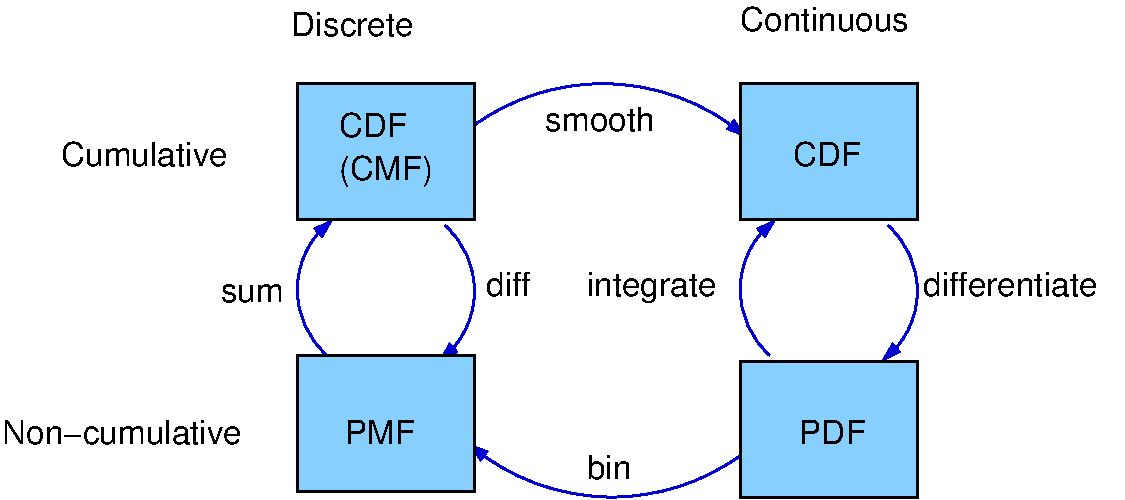
\includegraphics[height=2.2in]{figs/distribution_functions.pdf}}
\caption{A framework that relates representations of distribution
functions.}
\label{dist_framework}
\end{figure}

At this point we have seen PMFs, CDFs and PDFs; let's take a minute
to review.  Figure~\ref{dist_framework} shows how these functions relate
to each other.
\index{PMF}

We started with PMFs, which represent the probabilities for a discrete
set of values.  To get from a PMF to a CDF, we computed a cumulative sum.
To be more consistent, a discrete CDF should be called a cumulative mass
function (CMF), but as far as I can tell no one uses that term.
\index{CDF}

To get from a CDF to a PMF, you can compute differences in cumulative
probabilities.
\index{PDF}

Similarly, a PDF is the derivative of a continuous CDF; or, equivalently,
a CDF is the integral of a PDF.  But remember that a PDF maps from
values to probability densities; to get a probability, you have to
integrate.
\index{discrete}
\index{continuous}

To get from a discrete to a continuous distribution, you can perform
various kinds of smoothing.  One form of smoothing is to assume that
the data come from an analytic continuous distribution
(like exponential or normal) and to estimate the parameters of that
distribution.  Another option is kernel density estimation.
\index{exponential distribution}
\index{distribution!exponential}
\index{normal distribution}
\index{distribution!normal}
\index{Gaussian distribution}
\index{distribution!Gaussian}
\index{bin}

The opposite of smoothing is discretizing, or quantizing.  If you
evaluate a PDF at discrete points, you can generate a PMF that is at
least an approximation of the PDF.  You can get a better approximation
using numerical integration.
\index{Bayesian estimation}
\index{estimation!Bayesian}




\section{Glossary}

\begin{itemize}

\item skewness: A characteristic of a distribution; intuitively, it
is a measure of how asymmetric the distribution is.
\index{skewness}

\item robust: A statistic is robust if it is relatively immune to the
  effect of outliers.
\index{robust}

\item illusory superiority: The tendency of people to imagine that
they are better than average.
\index{illusory superiority}
\index{fallacy!illusory superiority}

\item random variable: An object that represents a random process.
\index{random variable}
\index{variable!random}

\item random variate: A value generated by a random process.
\index{random variate}
\index{variate!random}

\item PDF: Probability density function, the derivative of a continuous CDF.
\index{PDF}
\index{probability density function}

\item convolution: An operation that computes the distribution of the
sum of values from two distributions. 
\index{convolution}

%\item Chi-squared distribution: The distribution of the sum of squared
%values from a normal distribution.

%\item Degrees of freedom: The number of values in a sample that are
%free to vary.

\item Central Limit Theorem: ``The supreme law of Unreason,'' according
to Sir Francis Galton, an early statistician.
\index{Central Limit Theorem}
\index{Galton, Francis}
\index{unreason, supreme law}

\end{itemize}



\chapter{Relationships between variables}

\section{Scatterplots}
\index{scatter plot}
\index{plot!scatter}
\index{pyplot}

In this chapter we look at relationships between variables.  For
example, you might expect that weight is related to height; people who
are taller tend to be heavier.

\begin{figure}
% brfss_corr.py
\centerline{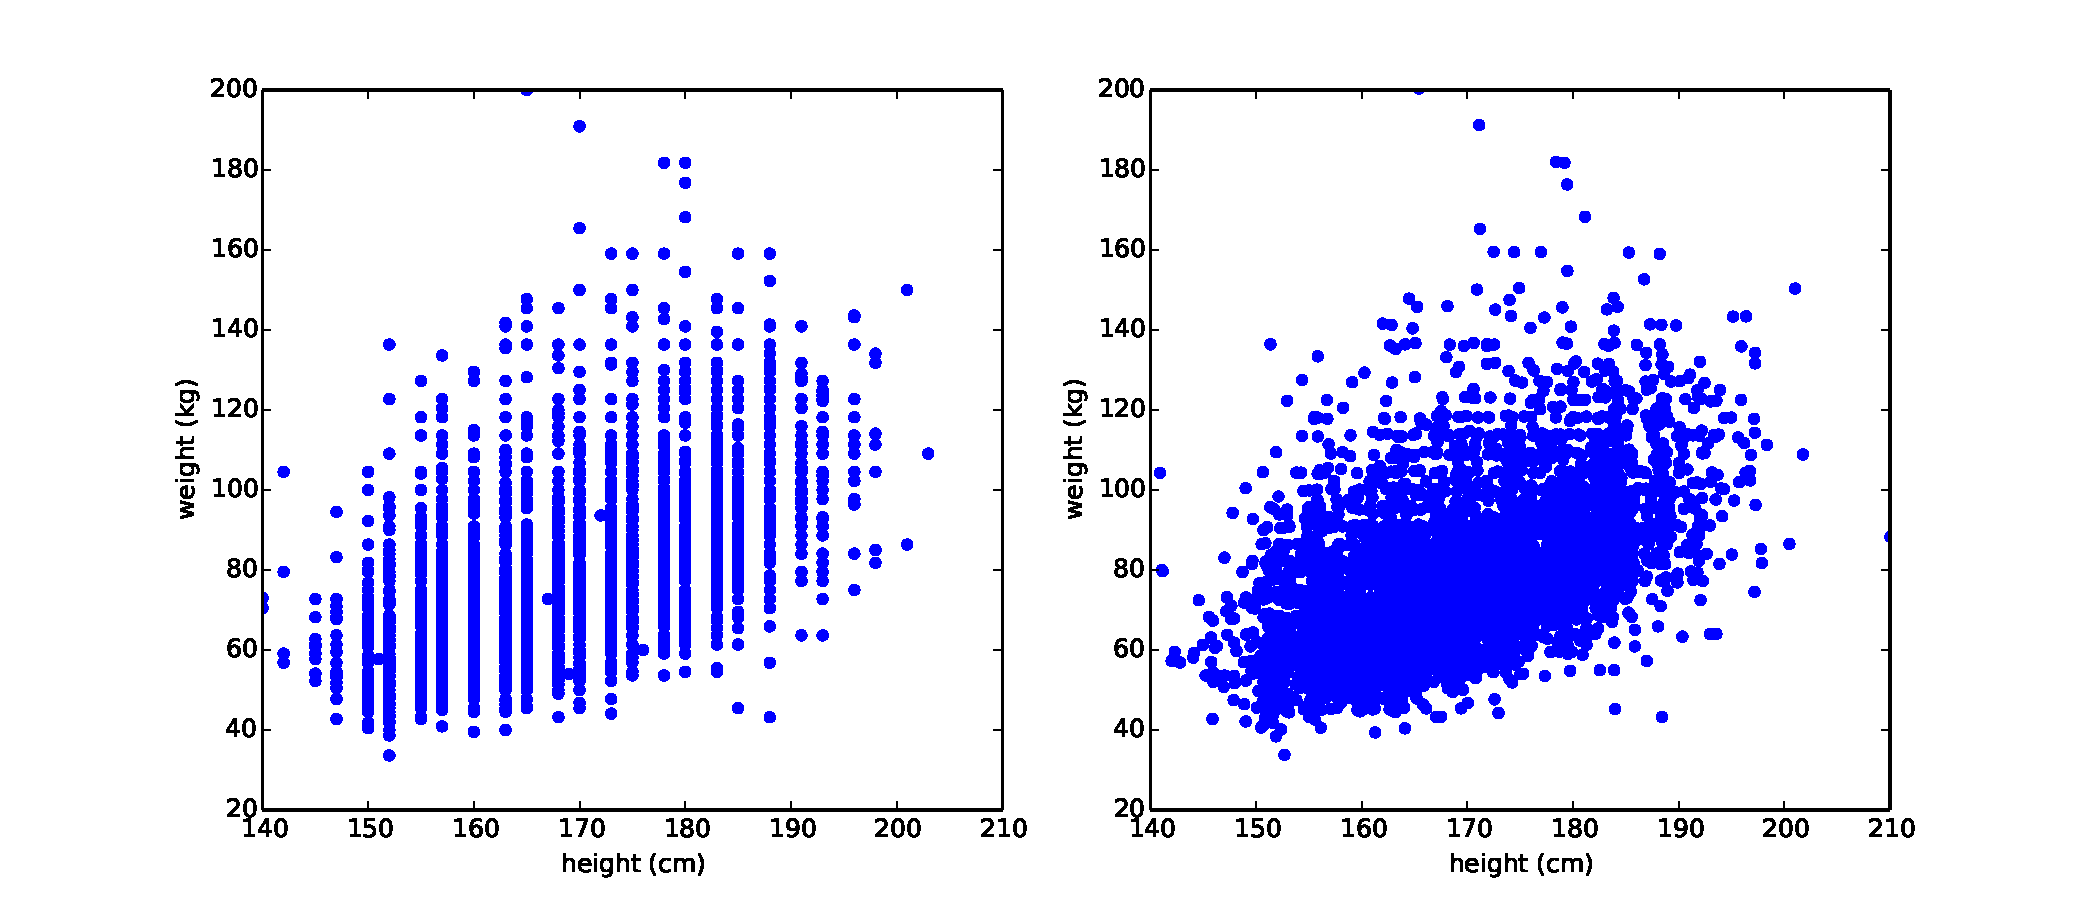
\includegraphics[height=2.5in]{figs/scatter1.pdf}}
\caption{Simple scatterplot of weight versus height for the respondents
in the BRFSS.}
\label{scatterplot1}
\end{figure}

\begin{figure}
% brfss_corr.py
\centerline{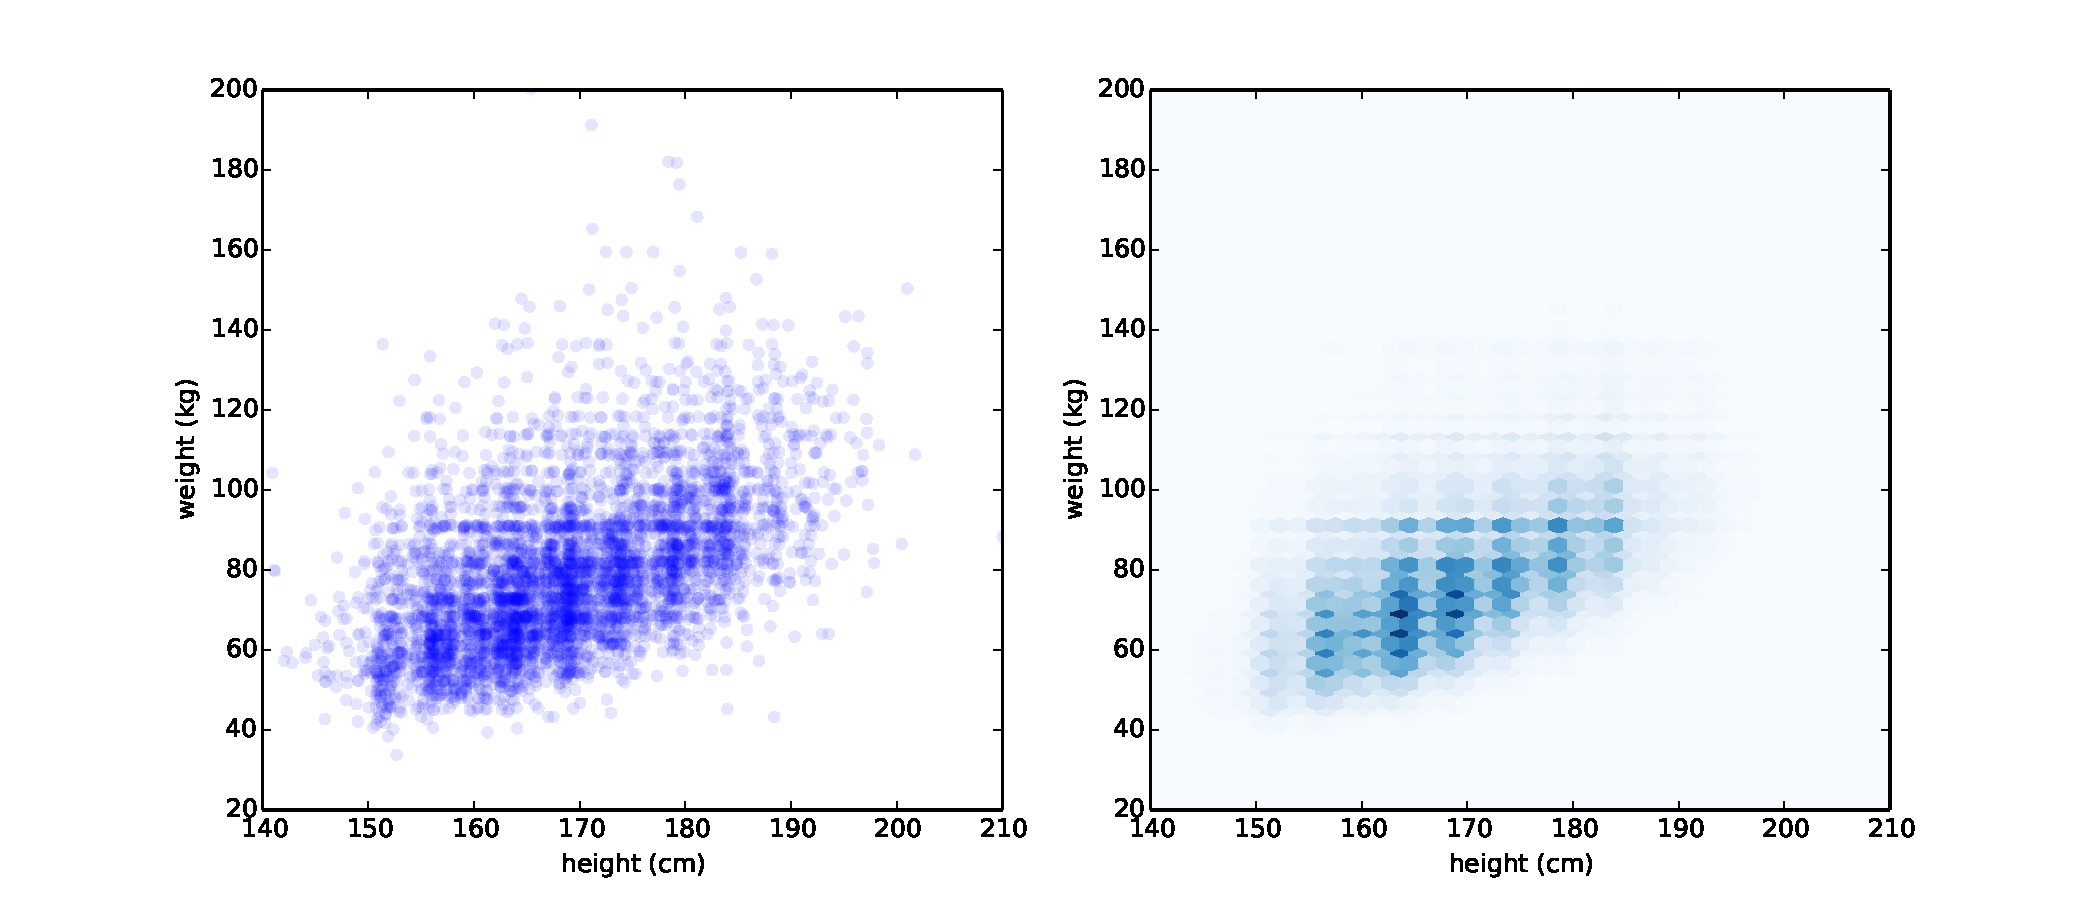
\includegraphics[height=2.5in]{figs/scatter2.pdf}}
\caption{Scatterplot with jittered data.}
\label{scatterplot2}
\end{figure}

\begin{figure}
% brfss_corr.py
\centerline{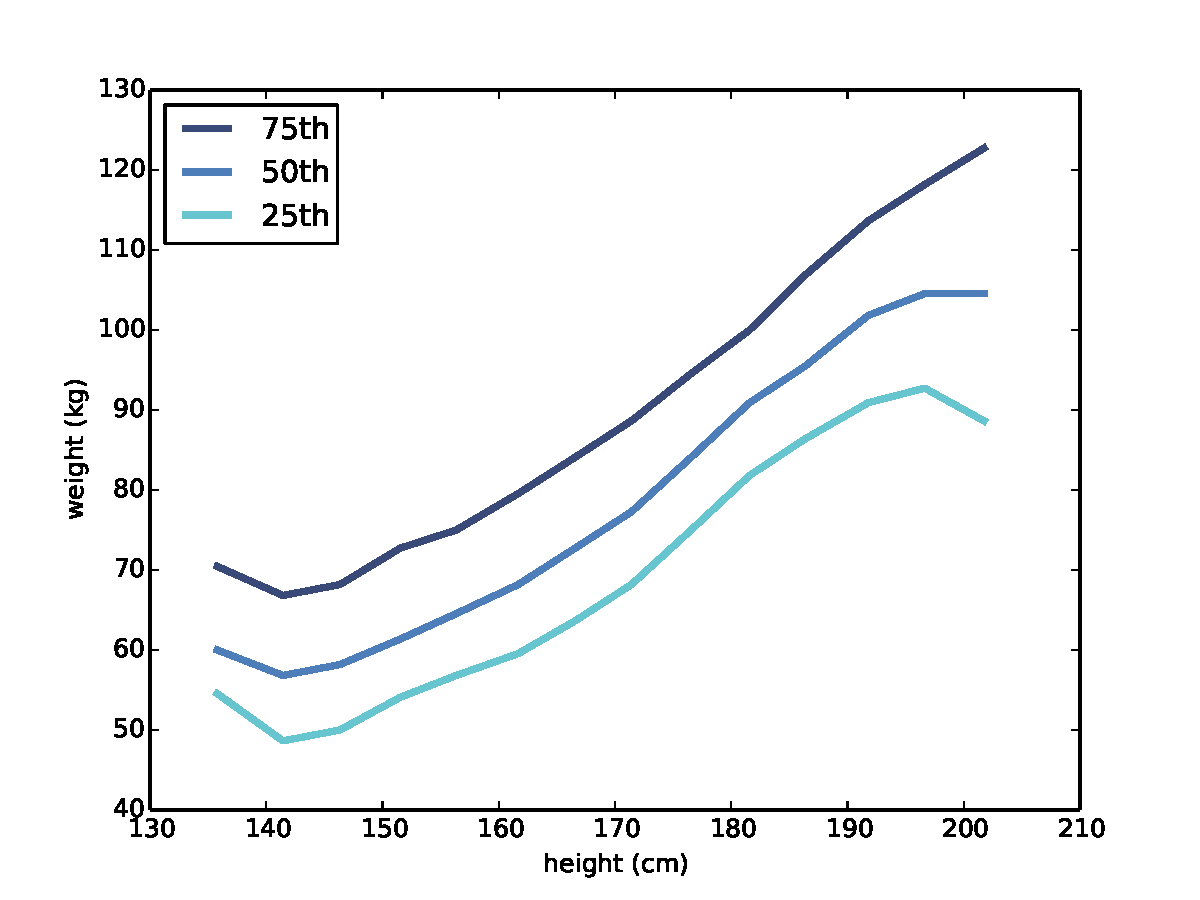
\includegraphics[height=2.5in]{figs/scatter3.pdf}}
\caption{Scatterplot with jittering and transparency.}
\label{scatterplot3}
\end{figure}

\begin{figure}
% brfss_corr.py
\centerline{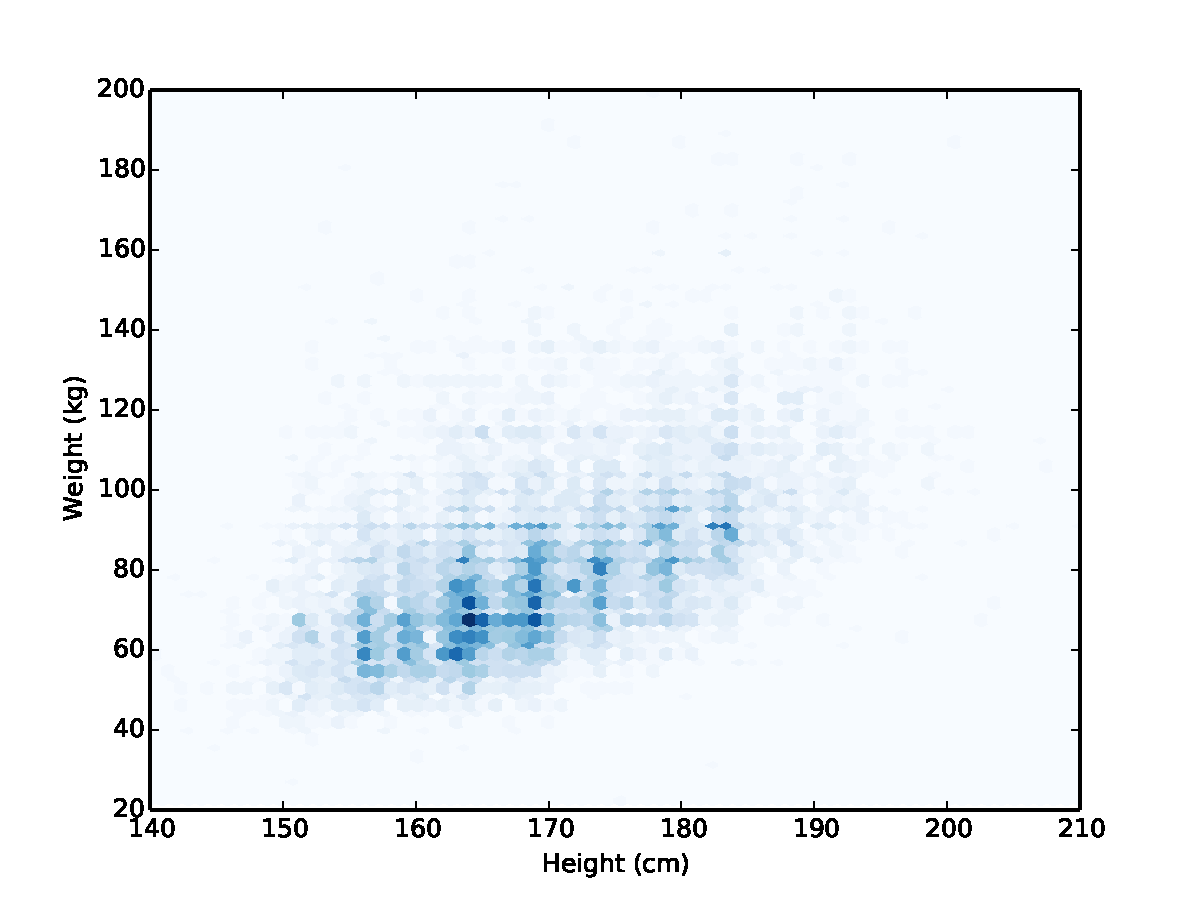
\includegraphics[height=2.5in]{figs/scatter4.pdf}}
\caption{Scatterplot with binned data using {\tt pyplot.hexbin}.}
\label{scatterplot4}
\end{figure}
\index{Behavioral Risk Factor Surveillance System}
\index{BRFSS}

The simplest way to check for a relationship between two variables
is a scatterplot, but making a good scatterplot is not always easy.
As an example, I'll plot weight versus height for the respondents
in the BRFSS (see Section~\ref{lognormal}).  {\tt pyplot} provides
a function named {\tt scatter} that makes scatterplots:
%
\begin{verbatim}
import matplotlib.pyplot as pyplot
pyplot.scatter(heights, weights)
\end{verbatim}

Figure~\ref{scatterplot1} shows the result.  Not surprisingly, taller
people tend to be heavier.  But this is not the best representation of
the data, because the data are packed into columns.  The problem is
that the heights were rounded to the nearest inch, converted to
centimeters, and then rounded again.  Some information is lost in
translation.  \index{height} \index{weight} \index{jitter}

We can't get that information back, but we can minimize the effect on
the scatterplot by {\bf jittering} the data, which means adding random
noise to reverse the effect of rounding off.  Since these measurements
were rounded to the nearest inch, they might be off by up to 0.5 inches or
1.3 cm.  So I added uniform noise in the range -1.3 to 1.3 cm:
\index{uniform distribution}
\index{distribution!uniform}
\index{noise}
%
\begin{verbatim}
jitter = 1.3
heights = [h + random.uniform(-jitter, jitter) for h in heights]
\end{verbatim}

Figure~\ref{scatterplot2} shows the result.  Jittering the data makes
the shape of the relationship clearer.  In general you should only jitter
data for purposes of visualization and avoid using jittered data
for analysis.

Even with jittering, this is not the best way to represent the data.
There are many overlapping points, which hides data
in the dense parts of the figure and gives disproportionate emphasis
to outliers.
\index{outlier}

We can solve this problem with the {\tt alpha} parameter, which makes
the points partly transparent:
%
\begin{verbatim}
pyplot.scatter(heights, weights, alpha=0.2)
\end{verbatim}
%
Figure~\ref{scatterplot3} shows the result.  Overlapping data
points look darker, so darkness is proportional to density.  In this
version of the plot we can see an apparent artifact: a horizontal line
near 90 kg or 200 pounds.  Since this data is based on self-reports in
pounds, the most likely explanation is that some responses were rounded off
(possibly down).

Using transparency works well for moderate-sized datasets, but this
figure only shows the first 1000 records in the BRFSS, out of a total
of 414509.
\index{hexbin plot}
\index{plot!hexbin}

To handle larger datasets, one option is a hexbin plot, which divides
the graph into hexagonal bins and colors each bin according to how many
data points fall in it.  {\tt pyplot} provides a function called 
{\tt hexbin}:
%
\begin{verbatim}
pyplot.hexbin(heights, weights, cmap=matplotlib.cm.Blues)
\end{verbatim}
%
Figure~\ref{scatterplot4} shows the result with a blue colormap.
An advantage of a hexbin is that it shows the shape of the relationship
well, and it is efficient for large datasets.  A drawback is that
it makes the outliers invisible.
\index{colormap}
\index{grayscale}

The moral of this story is that it is
not easy to make a scatterplot that shows the relationship clearly
without introducing misleading artifacts.
You can download the code for these figures from
\url{http://thinkstats2.com/brfss_scatter.py}.
\index{{\tt brfss\_scatter.py}}


\section{Correlation}

If the relationship between variables is linear, you can measure
the strength of the relationship by computing one of several
correlation statistics.

A challenge in measuring correlation is that the variables we want
to compare might not be expressed in the same units.  For example, height
might be in centimeters and weight in kilograms.  And even if they are
in the same units, they come from different distributions.
\index{units}

There are two common solutions to these problems:

\begin{enumerate}

\item Transform all values to {\bf standard scores}.  This leads to
the Pearson coefficient of correlation.
\index{standard scores}
\index{Pearson coefficient of correlation}
\index{Spearman coefficient of correlation}
\index{coefficient!correlation}

\item Transform all values to their percentile ranks.  This
leads to the Spearman coefficient.
\index{rank}
\index{percentile rank}

\end{enumerate}

If $X$ is a series of values, $x_i$, we can convert to standard
scores by subtracting the mean and dividing by the standard deviation:
$z_i = (x_i - \mu) / \sigma$.
\index{mean}
\index{standard deviation}

The numerator is a deviation: the distance from the mean.  Dividing by
$\sigma$ {\bf normalizes} the deviation, so the values of $Z$ are
dimensionless (no units) and their distribution has mean 0 and
variance 1.
\index{normalize}
\index{deviation}
\index{normal distribution}
\index{distribution!normal}
\index{Gaussian distribution}
\index{distribution!Gaussian}

If $X$ is normally distributed, so is $Z$; but if $X$ is skewed or has
outliers, so does $Z$.  In those cases it is more robust to use
percentile ranks.  If we compute a new variable, $R$, so that $r_i$ is
the percentile rank of $x_i$, the distribution of $R$ is uniform
between 0 and 100, regardless of the distribution of $X$.
\index{uniform distribution} \index{distribution!uniform}
\index{robust}


\section{Covariance}
\index{covariance}
\index{deviation}

{\bf Covariance} is a measure of the tendency of two variables
to vary together.  If we have two series, $X$ and $Y$, their
deviations from the mean are

\[ dx_i = x_i - \xbar \]

\[ dy_i = y_i - \ybar \]

where $\xbar$ is the sample mean of $X$ and $\ybar$ is the sample mean
of $Y$.  If $X$ and $Y$ vary together, their deviations tend to have
the same sign.

If we multiply them together, the product is positive when the
deviations have the same sign and negative when they have the opposite
sign.  So adding up the products gives a measure of the tendency to
vary together.

Covariance is the mean of these products:
%
\[ Cov(X,Y) = \frac{1}{n} \sum dx_i dy_i \]
%
where $n$ is the length of the two series (they have to be the same
length).

\begin{exercise}
Write a function called {\tt Cov} that takes two lists
and computes their covariance.  To test your function, compute
the covariance of a list with itself and confirm that
$Cov(X, X) = Var(X)$.

You can download a solution from
\url{http://thinkstats2.com/correlation.py}.
\index{{\tt correlation.py}}

\end{exercise}


\section{Pearson's correlation}
\index{correlation}
\index{standard score}

Covariance is useful in some computations, but
it is seldom reported as a summary statistic because it is hard to
interpret.  Among other problems, its units are the product of the
units of $X$ and $Y$.  So the covariance of weight and height might be
in units of kilogram-meters, which doesn't mean much.

One solution to this problem is to divide the deviations by $\sigma$,
which yields standard scores, and compute the product of standard scores:
%
\[ p_i = \frac{(x_i - \xbar)}{S_X} \frac{(y_i - \ybar)}{S_Y} \]
%
Where $S_X$ and $S_Y$ are the standard deviations of $X$ and $Y$.
The mean of these products is
%
\[ \rho = \frac{1}{n} \sum p_i \]
%
Or we can rewrite $\rho$ by factoring out $S_X$ and
$S_Y$:
%
\[ \rho = \frac{Cov(X,Y)}{S_X S_Y} \]
%
This value is called {\bf Pearson's correlation} after Karl Pearson,
an influential early statistician.  It is easy to compute and easy to
interpret.  Because standard scores are dimensionless, so is $\rho$.
\index{Pearson, Karl}
\index{Pearson coefficient of correlation}
\index{coefficient!correlation}

Pearson's correlation is always between -1 and +1 (including both).
If $\rho$ is positive, we say that the correlation is positive,
which means that when one variable is high, the other tends to be
high.  If $\rho$ is negative, the correlation is negative, so
when one variable is high, the other is low.

The magnitude of $\rho$ indicates the strength of the correlation.  If
$\rho$ is 1 or -1, the variables are perfectly correlated, which means
that if you know one, you can make a perfect prediction about the
other.  \index{prediction}

Most correlation in the real world is not perfect, but it
is still useful.  For example, if you know someone's height, you might
be able to guess their weight.  You might not get it exactly right, but
your guess will be better than if you didn't know the height.
Correlation is a measure of how much better.

So if $\rho = 0$, does that mean there is no
relationship between the variables?  Unfortunately, no.  Pearson's
correlation only measures {\em linear} relationships.  If there's a
nonlinear relationship, $\rho$ understates its strength.
\index{linear relationship}

\begin{figure}
% descriptive.py
\centerline{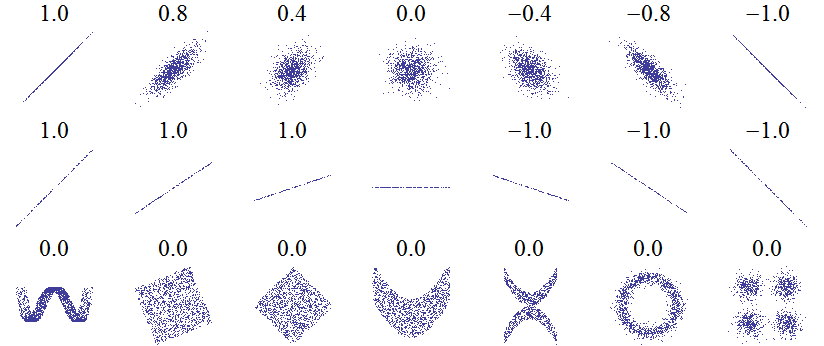
\includegraphics[height=2.5in]{figs/Correlation_examples.png}}
\caption{Examples of datasets with a range of correlations.}
\label{corr_examples}
\end{figure}

Figure~\ref{corr_examples} is from
\url{http://wikipedia.org/wiki/Correlation_and_dependence}.  It shows
scatterplots and correlation coefficients for several
carefully-constructed datasets.
\index{coefficient!correlation}
\index{scatter plot}
\index{plot!scatter}

The top row shows linear relationships with a range of correlations;
you can use this row to get a sense of what different values of
$\rho$ look like.  The second row shows perfect correlations with a
range of slopes, which demonstrates that correlation is unrelated to
slope (we'll talk about estimating slope soon).  The third row shows
variables that are clearly related, but because the relationship is
non-linear, the correlation coefficient is 0.

The moral of this story is that you should always look at a scatterplot of
your data before blindly computing a correlation coefficient.
\index{correlation coefficient}
\index{coefficient!correlation}

\begin{exercise}
Write a function called {\tt Corr} that takes two lists and
computes their correlation.  Hint: use {\tt thinkstats.Var} and
the {\tt Cov} function you wrote in the previous exercise.
\index{variance}
\index{covariance}

To test your function, compute the covariance of a list with itself
and confirm that $\Corr(X, X)$ is 1.  You can download a solution
from \url{http://thinkstats2.com/correlation.py}.
\index{{\tt correlation.py}}

\end{exercise}


\section{Spearman's rank correlation}

Pearson's correlation works well if the relationship between variables
is linear and if the variables are roughly normal.  But it is not
robust in the presence of outliers.
\index{Pearson coefficient of correlation}
\index{Spearman coefficient of correlation}
\index{coefficient!correlation}
\index{normal distribution}
\index{distribution!normal}
\index{Gaussian distribution}
\index{distribution!Gaussian}

Anscombe's quartet demonstrates this effect; it contains four data
sets with the same correlation.  One is a linear relation with random
noise, one is a non-linear relation, one is a perfect relation with an
outlier, and one has no relation except an artifact caused by an
outlier.  You can read more about it at
\url{http://wikipedia.org/wiki/Anscombe's_quartet}.
\index{Anscombe's quartet}

Spearman's rank correlation is an alternative that mitigates the
effect of outliers and skewed distributions.  To compute Spearman's
correlation, we have to compute the {\bf rank} of each value, which is its
index in the sorted sample.  For example, in the sample \{1, 2, 5, 7\}
the rank of the value 5 is 3, because it appears third in the sorted
list.  Then we compute Pearson's correlation for the ranks.

An alternative way to quantify correlation is to apply a transform
that makes the data more nearly normal, then compute Pearson's
correlation for the transformed data.  For example, if the data are
approximately lognormal, you could take the log of each value and
compute the correlation of the logs.  \index{lognormal distribution}
\index{distribution!lognormal}

\begin{exercise}
Write a function that takes a sequence and returns a list that
contains the rank for each element.  For example, if the sequence is
\{7, 1, 2, 5\}, the result should be \{ 4, 1, 2, 3\}.

If the same value appears more than once, the strictly correct
solution is to assign each of them the average of their ranks.  But if
you ignore that and assign them ranks in arbitrary order, the error is
usually small.

Write a function that takes two sequences (with the same length) and
computes their Spearman rank coefficient.  You can download a solution
from \url{http://thinkstats2.com/correlation.py}.
\index{{\tt correlation.py}}
\index{Spearman coefficient of correlation}
\index{coefficient!correlation}

\end{exercise}


\begin{exercise}
Download \url{http://thinkstats2.com/brfss.py} and
\url{http://thinkstats2.com/brfss_scatter.py}.  Run them and confirm that you
can read the BRFSS data and generate scatterplots.
\index{Behavioral Risk Factor Surveillance System}
\index{BRFSS}
\index{{\tt brfss.py}}
\index{{\tt brfss\_scatter.py}}

Comparing the scatterplots to Figure~\ref{corr_examples}, what value
do you expect for Pearson's correlation?  What value do you get?
\index{weight!adult}
\index{adult weight}
\index{lognormal distribution}
\index{distribution!lognormal}
\index{outlier}

Because the distribution of adult weight is lognormal, there are
outliers that affect the correlation.  Try plotting
log(weight) versus height, and compute Pearson's
correlation for the transformed variable.

Finally, compute Spearman's rank correlation for weight and height.
Which coefficient do you think is the best measure of the strength of
the relationship?  You can download a solution from
\url{http://thinkstats2.com/brfss_corr.py}.
\index{{\tt brfss\_corr.py}}

\end{exercise}


\section{Least squares fit}

Correlation coefficients measure the strength and sign of a
relationship, but not the slope.  There are several ways to estimate
the slope; the most common is a {\bf linear least squares fit}.  A
``linear fit'' is a line intended to model the relationship between
variables.  A ``least squares'' fit is one that minimizes the mean
squared error (MSE) between the line and the data\footnote{See
  \url{http://wikipedia.org/wiki/Simple_linear_regression}.}.
\index{least squares fit}
\index{linear least squares}
\index{coefficient!correlation}
\index{linear regression}

Suppose we have a sequence of points, $Y$, that we want to express as a
function of another sequence $X$.  If there is a linear relationship
between $X$ and $Y$ with intercept $\alpha$ and slope $\beta$, we
expect each $y_i$ to be roughly $\alpha + \beta x_i$.
\index{residual}

But unless the correlation is perfect, this prediction is only
approximate.  The deviation, or {\bf residual}, is 

\[ \eps_i = (\alpha + \beta x_i) - y_i \]

The residual might be due to random factors like measurement error,
or non-random factors that are unknown.  For example, if we are
trying to predict weight as a function of height, unknown factors
might include diet, exercise, and body type.
\index{slope}
\index{intercept}

If we get the parameters $\alpha$ and $\beta$ wrong, the residuals
get bigger, so it makes intuitive sense that the parameters we want
are the ones that minimize the residuals.

As usual, we could minimize the absolute value of the
residuals, or their squares, or their cubes, etc.  The most common
choice is to minimize the sum of squared residuals
%
\[ \min_{\inter, \slope} \sum \eps_i^2 \]
%
Why?  There are three good reasons and one bad one:

\begin{itemize}

\item Squaring has the obvious feature of treating positive and
negative residuals the same, which is usually what we want.

\item Squaring gives more weight to large residuals, but not
so much weight that the largest residual always dominates.

\item If the residuals are independent of $x$, random, and normally
  distributed with $\mu = 0$ and constant (but unknown) $\sigma$, then
  the least squares fit is also the maximum likelihood estimator of
  $\alpha$ and $\beta$.\footnote{See Press et al., {\em Numerical Recipes in C},
    Chapter 15 at \url{http://www.nrbook.com/a/bookcpdf/c15-1.pdf}.}
\index{MLE}
\index{maximum likelihood estimator}

\item The values of $\hat{\inter}$ and $\hat{\slope}$ that minimize
  the squared residuals can be computed efficiently.

\end{itemize}

That last reason made sense when computational efficiency was more
important than choosing the method most appropriate to the problem
at hand.  That's no longer the case, so it is worth considering
whether squared residuals are the right thing to minimize.
\index{computation}

For example, if you are using values of $X$ to predict values of $Y$,
guessing too high might be better (or worse) than guessing too low.
In that case you might want to compute some cost function,
cost(\_i), and minimize total cost.
\index{cost function}

However, computing a least squares fit is quick, easy and often good
enough, so here's how:

\begin{enumerate}

\item Compute the sample means, $\xbar$ and $\ybar$, the variance
of $X$, and the covariance of $X$ and $Y$.

\item The estimated slope is
%
\[ \hat{\slope} = \frac{Cov(X,Y)}{Var(X)} \]
%
\item And the intercept is
%
\[ \hat{\inter} = \ybar - \hat{\slope} \xbar \]
%
\end{enumerate}

To see how this is derived, you can read
\url{http://wikipedia.org/wiki/Numerical_methods_for_linear_least_squares}.


\begin{exercise}
Write a function named {\tt LeastSquares} that takes $X$ and $Y$ and
computes $\hat{\inter}$ and $\hat{\slope}$.  You can download a
solution from \url{http://thinkstats2.com/correlation.py}.  \index{{\tt
    correlation.py}}

\end{exercise}

\begin{exercise}
Using the data from the BRFSS again, compute the linear least squares
fit for log(weight) versus height.  You can download a
solution from \url{http://thinkstats2.com/brfss_corr.py}.
\index{Behavioral Risk Factor Surveillance System}
\index{BRFSS}
\index{{\tt brfss\_corr.py}}

\end{exercise}


\begin{exercise}
The distribution of wind speeds in a given location determines the
wind power density, which is an upper bound on the average power that
a wind turbine at that location can generate.  According to some
sources, empirical distributions of wind speed are well modeled by a
Weibull distribution (see
\url{http://wikipedia.org/wiki/Wind_power#Distribution_of_wind_speed}).
\index{wind speed}
\index{wind power density}
\index{turbine}
\index{Weibull distribution}
\index{distribution!Weibull}

To evaluate whether a location is a viable site for a wind turbine,
you can set up an anemometer to measure wind speed for a period of
time.  But it is hard to measure the tail of the wind speed distribution
accurately because, by definition, events in the tail don't happen
very often.
\index{tail}

One way to address this problem is to use measurements to estimate the
parameters of a Weibull distribution, then integrate over the
continuous PDF to compute wind power density.
\index{PDF}

To estimate the parameters of a Weibull distribution, we can use the
transformation from Exercise~\ref{weibull} and then use a linear fit
to find the slope and intercept of the transformed data.

Write a function that takes a sample from a Weibull distribution and
estimates its parameters.

Now write a function that takes the parameters of a Weibull distribution
of wind speed and computes average wind power density (you might have
to do some research for this part).

\end{exercise}


\section{Goodness of fit}
\index{goodness of fit}
\index{fit, goodness}

Having fit a linear model to the data, we might want to know how good
it is.  Well, that depends on what it's for.  One way to evaluate a
model is its predictive power.

In the context of prediction, the quantity we are trying to guess is
called a {\bf dependent variable} and the quantity we are using to
make the guess is called an {\bf explanatory} or {\bf independent
  variable}.
\index{dependent variable}
\index{explanatory variable}
\index{independent variable}
\index{coefficient!determination}

To measure the predictive power of a model, we can compute the {\bf
  coefficient of determination}, more commonly known as ``R-squared'':
%
\[ R^2 = 1 - \frac{Var(\eps)}{Var(Y)}\]
%
To understand what $R^{2}$ means, suppose (again) that you are trying
to guess someone's weight.  If you didn't know anything about them,
your best strategy would be to guess $\ybar$; in
that case the MSE of your guesses would be $Var(Y)$:
%
\[ MSE = \frac{1}{n} \sum (\ybar - y_i)^2 = Var(Y) \]
%
But if I told you their height, you would guess $\hat{\inter} +
\hat{\slope} x_i$; in that case your MSE would be $Var(\eps)$.
%
\[ MSE = 
\frac{1}{n} \sum (\hat{\inter} + \hat{\slope} x_i - y_i)^2 =
Var(\eps) \]
%
So the term $Var(\eps)/Var(Y)$ is the ratio of mean squared error with
and without the explanatory variable, which is the fraction of
variability left unexplained by the model.  The complement, $R^{2}$,
is the fraction of variability explained by the model.
\index{variability}

If a model yields $R^{2} = 0.64$, you could say that the model explains
64\% of the variability, or it might be more precise to say that it
reduces the MSE of your predictions by 64\%.

In the context of a linear least squares model, it turns out that
there is a simple relationship between the coefficient of
determination and Pearson's correlation coefficient, $\rho$:

\[ R^{2} = \rho^{2}\]

See \url{http://wikipedia.org/wiki/Howzzat}!
\index{howzzat}

\begin{exercise}
The Wechsler Adult Intelligence Scale (WAIS) is meant to be a measure
of intelligence; scores are calibrated so that the mean and standard
deviation in the general population are 100 and 15.
\index{Adult Intelligence Scale}
\index{WAIS}
\index{IQ}
\index{intelligence}

Suppose that you wanted to predict someone's WAIS score based on their
SAT scores.  According to one study, there is a Pearson correlation of
0.72 between total SAT scores and WAIS scores.

If you applied your predictor to a large sample, what would you expect to
be the mean squared error (MSE) of your predictions?

Hint: What is the MSE if you always guess 100?
\end{exercise}


\begin{exercise}
Write a function named {\tt Residuals} that takes X, Y, $\hat{\inter}$
and $\hat{\slope}$ and returns a list of $\eps_i$.
\index{residual}

Write a function named {\tt CoefDetermination} that takes the 
$\eps_i$ and Y and returns $R^{2}$.  To test your functions, 
confirm that $R^{2} = \rho^{2}$.  You can download a solution
from \url{http://thinkstats2.com/correlation.py}.
\index{{\tt correlation.py}}

\end{exercise}

\begin{exercise}
Using the height and weight data from the BRFSS (one more time),
compute $\hat{\inter}$, $\hat{\slope}$ and $R^{2}$.  If you were trying to guess
someone's weight, how much would it help to know their height?
You can download a solution from
\url{http://thinkstats2.com/brfss_corr.py}.
\index{Behavioral Risk Factor Surveillance System}
\index{BRFSS}
\index{{\tt brfss\_corr.py}}

\end{exercise}


\section{Correlation and Causation}
\index{correlation}
\index{causation}
\index{xkcd}
\index{comic}
\index{Munroe, Randall}

The web comic {\tt xkcd} demonstrates the difficulty of inferring
causation:

\begin{figure}
\centerline{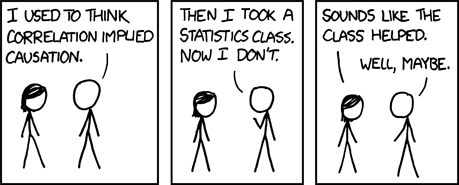
\includegraphics[width=4.0in]{figs/correlation.png}}
\caption{From {\tt xkcd.com} by Randall Munroe.}
\end{figure}

In general, a relationship between two variables does not tell you
whether one causes the other, or the other way around, or both, or
whether they might both be caused by something else altogether.

This rule can be summarized with the phrase ``Correlation
does not imply causation,'' which is so pithy it has its own
Wikipedia page: \url{http://wikipedia.org/wiki/Correlation_does_not_imply_causation}.

So what can you do to provide evidence of causation?

\begin{enumerate}

\item Use time.  If A comes before B, then A can cause B but not the
  other way around (at least according to our common understanding of
  causation).  The order of events can help us infer the direction
  of causation, but it does not preclude the possibility that something
  else causes both A and B.

\item Use randomness.  If you divide a large population into two
  groups at random and compute the means of almost any variable, you
  expect the difference to be small.  This is a consequence of the
  Central Limit Theorem (so it is subject to the same requirements).

  If the groups are nearly identical in all variable but one, you
  can eliminate spurious relationships.
\index{spurious relationship}

  This works even if you don't know what the relevant variables
  are, but it works even better if you do, because you can check that
  the groups are identical.

\end{enumerate}

These ideas are the motivation for the {\bf randomized controlled
trial}, in which subjects are assigned randomly to two (or more)
groups: a {\bf treatment} group that receives some kind of intervention,
like a new medicine, and a {\bf control group} that receives
no intervention, or another treatment whose effects are known.
\index{randomized controlled trial}
\index{controlled trial}
\index{treatment group}
\index{control group}
\index{medicine}

A randomized controlled trial is the most reliable way to demonstrate
a causal relationship, and the foundation of science-based medicine
(see \url{http://wikipedia.org/wiki/Randomized_controlled_trial}).

Unfortunately, controlled trials are only possible in the laboratory
sciences, medicine, and a few other disciplines.  In the social sciences,
controlled experiments are rare, usually because they are impossible
or unethical.

One alternative is to look for a {\bf natural experiment}, where
different ``treatments'' are applied to groups that are otherwise
similar.  One danger of natural experiments is that the groups might
differ in ways that are not apparent.  You can read more about this
topic at \url{http://wikipedia.org/wiki/Natural_experiment}.
\index{natural experiment}

In some cases it is possible to infer causal relationships using {\bf
  regression analysis}.  A linear least squares fit
is a simple form of regression that explains a dependent
variable using one explanatory variable.  There are similar
techniques that work with arbitrary numbers of independent variables.
\index{regression analysis}

I won't cover those techniques here, but there are also simple ways to
control for spurious relationships.  For example, in the NSFG, we saw
that first babies tend to be lighter than others (see
Section~\ref{birth_weights}).  But birth weight is also correlated
with the mother's age, and mothers of first babies tend to be younger
than mothers of other babies.
\index{birth weight}
\index{weight!birth}
\index{National Survey of Family Growth}
\index{NSFG}

So it may be that first babies are lighter because their mothers are
younger.  To control for the effect of age, we could divide the mothers
into age groups and compare birth weights for first babies and others
in each age group.
\index{pooled data}

If the difference between first babies and others is the same in
each age group as it was in the pooled data, we conclude
that the difference is not related to age.  If there is no difference,
we conclude that the effect is entirely due to age.  Or,
if the difference is smaller, we can quantify how much of the effect
is due to age.

\begin{exercise}
The NSFG data includes a variable named {\tt agepreg} that records
the age of the mother at the time of birth.
Make a scatterplot of mother's age and baby's weight for each live
birth.  Can you see a relationship?

Compute a linear least-squares fit for these variables.  What are the
units of the estimated parameters $\hat{\inter}$ and $\hat{\slope}$?
How would you summarize these results in a sentence or two?

Compute the average age for mothers of first babies and the average
age of other mothers.  Based on the difference in ages between the
groups, how much difference do you expect in the mean birth weights?
What fraction of the actual difference in birth weights is explained
by the difference in ages?

You can download a solution to this problem from
\url{http://thinkstats2.com/agemodel.py}.  If you are curious about
multivariate regression, you can run \url{http://thinkstats2.com/age_lm.py}
which shows how to use the R statistical computing package from
Python.  But that's a whole other book.
\index{{\tt agemodel.py}}
\index{{\tt age\_lm.py}}

\end{exercise}


\section{Glossary}

\begin{itemize}

\item correlation: a description of the dependence between variables.
\index{correlation}

\item normalize: To transform a set of values so that their mean is 0 and
their variance is 1.
\index{normalize}

\item standard score: A value that has been normalized.
\index{standard score}

\item covariance: a measure of the tendency of two variables
to vary together.
\index{covariance}

\item rank: The index where an element appears in a sorted list.
\index{rank}

\item least squares fit: A model of a dataset that minimizes the
sum of squares of the residuals.
\index{least squares fit}

\item residual: A measure of the deviation of an actual value from a model.
\index{residual}

\item dependent variable: A variable we are trying to predict or explain.
\index{dependent variable}

\item independent variable: A variable we are using to predict a dependent
variable, also called an explanatory variable.
\index{independent variable}

\item coefficient of determination: A measure of the goodness of fit
of a linear model.
\index{coefficient!determination}

\item randomized controlled trial: An experimental design in which subject
are divided into groups at random, and different groups are given different
treatments.
\index{randomized controlled trial}

\item treatment: An change or intervention applied to one group in a
controlled trial.
\index{treatment group}

\item control group: A group in a controlled trial that receives no
treatment, or a treatment whose effect is known.
\index{control group}

\item natural experiment: An experimental design that takes advantage of
a natural division of subjects into groups in ways that are at least
approximately random.
\index{natural experiment}

\end{itemize}




\chapter{Estimation}
\label{estimation}
\index{estimation}

\section{The estimation game}

Let's play a game.  I'll think of a distribution, and you have to guess
what it is.  I'll give you two hints; it's a
normal distribution, and here's a random sample drawn from it:
\index{normal distribution}
\index{distribution!normal}
\index{Gaussian distribution}
\index{distribution!Gaussian}

\{-0.441, 1.774, -0.101, -1.138, 2.975, -2.138\}

What do you think is the mean parameter, $\mu$, of this distribution?
\index{mean}
\index{parameter}

One choice is to use the sample mean, $\xbar$, as an estimate of $\mu$.
In this example, $\xbar$ is 0.155, so it would
be reasonable to guess $\mu$ = 0.155.
This process is called {\bf estimation}, and the statistic we used
(the sample mean) is called an {\bf estimator}.
\index{estimator}

Using the sample mean to estimate $\mu$ is so obvious that it is hard
to imagine a reasonable alternative.  But suppose we change the game by
introducing outliers.
\index{normal distribution}
\index{distribution!normal}
\index{Gaussian distribution}
\index{distribution!Gaussian}

{\em I'm thinking of a distribution.}  It's a normal distribution, and
here's a sample that was collected by an unreliable surveyor who
occasionally puts the decimal point in the wrong place.

\{-0.441, 1.774, -0.101, -1.138, 2.975, -213.8\}

Now what's your estimate of $\mu$?  If you use the sample mean, your
guess is -35.12.  Is that the best choice?  What are the alternatives?
\index{outlier}

One option is to identify and discard outliers, then compute the sample
mean of the rest.  Another option is to use the median as an estimator.
\index{median}

Which estimator is best depends on the circumstances (for example,
whether there are outliers) and on what the goal is.  Are you
trying to minimize errors, or maximize your chance of getting the
right answer?
\index{error}
\index{MSE}
\index{mean squared error}

If there are no outliers, the sample mean minimizes the {\bf mean squared
error} (MSE).  That is, if we play the game many times, and each time
compute the error $\xbar - \mu$, the sample mean minimizes
%
\[ MSE = \frac{1}{m} \sum (\xbar - \mu)^2 \]
%
Where $m$ is the number of times you play the estimation game (not to
be confused with $n$, which is the size of the sample used to compute
$\xbar$).

Here is a function that simulates the estimation game and computes
the root mean squared error (RMSE), which is the square root of
MSE:

\begin{verbatim}
def Estimate1(n=7, m=1000):
    mu = 0
    sigma = 1

    means = []
    medians = []
    for _ in range(m):
        xs = [random.gauss(mu, sigma) for i in range(n)]
        xbar = numpy.mean(xs)
        median = thinkstats2.Median(xs)
        means.append(xbar)
        medians.append(median)

    print 'rmse xbar', RMSE(means, mu)
    print 'rmse median', RMSE(medians, mu)
\end{verbatim}

Again, {\tt n} is the size of the sample, and {\tt m} is the
number of times we play the game.  {\tt means} is the list of
estimates based on $\xbar$.  {\tt medians} is the list of medians.

Here's the function that computes RMSE:

\begin{verbatim}
def RMSE(estimates, actual):
    e2 = [(estimate-actual)**2 for estimate in estimates]
    mse = numpy.mean(e2)
    return math.sqrt(mse)
\end{verbatim}

{\tt estimates} is a list of estimates; {\tt actual} is the
actual value being estimated.  In practice, of course, we don't
know {\tt actual}; if we did, we wouldn't have to estimate it.
The purpose of this experiment is to compare the performance of
the two estimators.

When I ran this code, the RMSE of the sample mean was 0.41, which
means that if we use $\xbar$ to estimate the mean of this
distribution, based on a sample with $n=7$, we should expect to be off
by 0.41 on average.  Using the median to estimate the mean yields
RMSE 0.53, which confirms that $\xbar$ yields lower RMSE, at least
for this example.

Minimizing MSE is a nice property, but it's not always the best
strategy.  For example, suppose we are estimating the distribution of
wind speeds at a building site.  If the estimate is too high, we might
overbuild the structure, increasing its cost.  But if it's too
low, the building might collapse.  Because cost as a function of
error is not symmetric, minimizing MSE is not the best strategy.
\index{prediction}

As another example, suppose I roll three six-sided dice and ask you to
predict the total.  If you get it exactly right, you get a prize;
otherwise you get nothing.  In this case the value that minimizes MSE
is 10.5, but that would be a bad guess, because the total of three
dice is never 10.5.  For this game, you want an estimator that has the
highest chance of being right, which is a {\bf maximum likelihood
  estimator} (MLE).  If you pick 10 or 11, your chance of winning is 1
in 8, and that's the best you can do.  \index{MLE} \index{maximum
  likelihood estimator}


\section{Guess the variance}
\index{variance}
\index{normal distribution}
\index{distribution!normal}
\index{Gaussian distribution}
\index{distribution!Gaussian}

{\em I'm thinking of a distribution.}  It's a normal distribution, and 
here's a (familiar) sample:

\{-0.441, 1.774, -0.101, -1.138, 2.975, -2.138\}

What do you think is the variance, $\sigma^2$, of my distribution?
Again, the obvious choice is to use the sample variance, $S^2$, as an
estimator.
%
\[ S^2 = \frac{1}{n} \sum (x_i - \xbar)^2 \] 
%
For large samples, $S^2$ is an adequate estimator, but for small
samples it tends to be too low.  Because of this unfortunate
property, it is called a {\bf biased} estimator.
An estimator is {\bf unbiased} if the expected total (or mean) error,
after many iterations of the estimation game, is 0.
\index{sample variance}
\index{biased estimator}
\index{estimator!biased}
\index{unbiased estimator}
\index{estimator!unbiased}

Fortunately, there is another simple statistic that is an unbiased
estimator of $\sigma^2$:
%
\[ S_{n-1}^2 = \frac{1}{n-1} \sum (x_i - \xbar)^2 \] 
%
The biggest problem with this estimator is that its name and symbol
are used inconsistently.  The name ``sample variance'' can refer to
either $S^2$ or $S_{n-1}^2$, and the symbol $S^2$ is used
for either or both.

For an explanation of why $S^2$ is biased, and a proof that
$S_{n-1}^2$ is unbiased, see
\url{http://wikipedia.org/wiki/Bias_of_an_estimator}.

Here is a function that simulates the estimation game and tests
the performance of $S^2$ and $S_{n-1}^2$:

\begin{verbatim}
def Estimate2(n=7, m=1000):
    mu = 0
    sigma = 1

    estimates1 = []
    estimates2 = []
    for _ in range(m):
        xs = [random.gauss(mu, sigma) for i in range(n)]
        biased = numpy.var(xs)
        unbiased = numpy.var(xs, ddof=1)
        estimates1.append(biased)
        estimates2.append(unbiased)

    print 'mean error biased', MeanError(estimates1, sigma**2)
    print 'mean error unbiased', MeanError(estimates2, sigma**2)
\end{verbatim}

Again, {\tt n} is the sample size and {\tt m} is the number of times
we play the game.  {\tt numpy.var} to computes $S^2$ by default and
$S_{n-1}^2$ if you provide the parameter {\tt ddof=1}, which stands for
``delta degrees of freedom.''  I won't explain that now, but if you
can't stand suspense, you can read
\url{http://en.wikipedia.org/wiki/Degrees_of_freedom_(statistics)}.

{\tt MeanError} computes the mean difference between the estimates
and the actual value:

\begin{verbatim}
def MeanError(estimates, actual):
    errors = [estimate-actual for estimate in estimates]
    return numpy.mean(errors)
\end{verbatim}

When I ran this code, the mean error for $S^2$ was -0.13.  As
expected, this biased estimator tends to be too low.  For $S_{n-1}^2$,
the mean error was 0.014, about 10 times smaller.  As {\tt m}
increases, we expect the mean error for $S_{n-1}^2$ to approach 0.

Properties like MSE and bias are long-term expectations based on
many iterations of the estimation game.  By running simulations like
the ones in this chapter, we can compare estimators and check whether
they have desired properties.

But when you apply an estimator to real
data, you just get one estimate.  It would not be meaningful to say
that the estimate is unbiased; being unbiased is a property of the
estimator, not the estimate.

If you choose an estimator with appropriate properties, and use it to
generate an estimate, the next step is to characterize the
uncertainty of the estimate, which is the topic of the next
section.

You can download code for these experiments from \url{}.

\begin{exercise}

So far we have used $\xbar$ and median to estimate $\mu$, and
found that $\xbar$  yields lower MSE.

As we used $S^2$ and $S_{n-1}^2$ to estimate $\sigma$, and found that
$S^2$ is biased and $S_{n-1}^2$ unbiased.

Run similar experiments to see if $\xbar$ and median are biased estimates
of $\mu$.

Also check whether $S^2$ or $S_{n-1}^2$ yields a lower MSE.

\end{exercise}


\section{Sampling distributions}

Suppose you are a primatologist studying gorillas in a wildlife
preserve.  You want to know the average weight of the adult
female gorillas in the preserve.  To weigh them, you have
to tranquilize them, which is dangerous, expensive, and possibly
harmful to the gorillas.  But if it is important to obtain this
information, it might be acceptable to weigh a sample of 9
gorillas.  Let's assume that the population of the preserve is
well known, so we can choose a representative sample of adult
females.  We could use the sample mean, $\xbar$, to estimate the
unknown population mean, $\mu$.

Having weighed 9 female gorillas, you might find $\xbar=90$ kg and
sample standard deviation, $S=7.5$ kg.  The sample mean, $\xbar=90$,
is an unbiased estimator of $\mu$, and in the long run it
minimizes MSE.  So if you reported a single
estimate that summarizes the results, you would report 90 kg.

But how confident should you be in this estimate?  If you only weigh
$n=9$ gorillas out of a much larger population, you might be unlucky
and choose the 9 heaviest gorillas (or the 9 lightest ones) just by
chance.  Variation in the estimate caused by random selection is
called {\bf sampling error}.

To quantify the size of the sampling error, we can simulate the
sampling process with hypothetical values of $\mu$ and $\sigma$, and
see how much $\xbar$ varies.

Since we don't know the actual values of 
$\mu$ and $\sigma$ in the population, we'll use the estimates
$\xbar$ and $S$.
So the question we answer is:
``If the actual values of $\mu$ and $\sigma$ were 90 kg and 7.5 kg,
and we ran the same experiment many times, how much would the
estimated mean, $\xbar$, vary?''

The following function answers that question:

\begin{verbatim}
def SimulateSample(mu=90, sigma=7.5, n=9, m=1000):
    
    means = []
    for j in range(m):
        xs = [random.gauss(mu, sigma) for i in range(n)]
        xbar = numpy.mean(xs)
        means.append(xbar)

    cdf = thinkstats2.MakeCdfFromList(means)
\end{verbatim}

{\tt mu} and {\tt sigma} are the {\em hypothetical} values of
the parameters.  {\tt n} is the sample size, the number of
gorillas we measured.  {\tt m} is the number of times we run
the simulation.

\begin{figure}
% estimate.py
\centerline{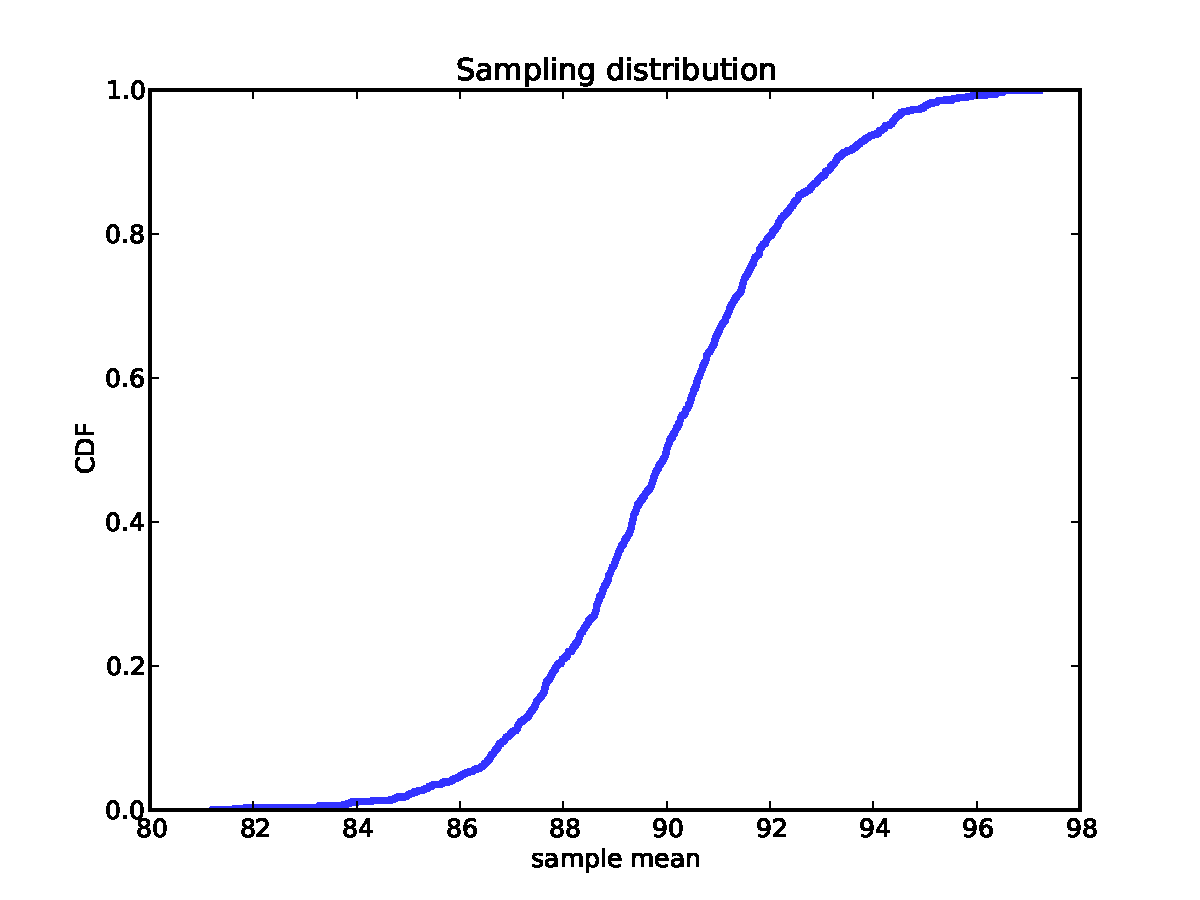
\includegraphics[height=2.5in]{figs/estimate1.pdf}}
\caption{Sampling distribution of $\xbar$.}
\label{fig.sampling}
\end{figure}

For each simulation, we choose {\tt n} values from a Gaussian
distribution with the given parameters, and compute the sample mean,
{\tt xbar}.  We run 1000 simulations and then compute the
distribution, {\tt cdf}, of the estimates.  The result is shown in
Figure~\ref{fig.sampling}.  This distribution is called the {\bf
  sampling distribution} of the estimator.  It shows how much the
estimates would vary if we ran the experiment over and over.

The mean of the sampling distribution is pretty close
to the hypothetical value of $\mu$, which means that the experiment
yields the right answer, on average.  After 1000 tries, the lowest
result is 82 kg, and the highest is 98 kg.  This range suggests that
the estimate might be off by 8 kg.  

But there are other ways to summarize the sampling distribution.
For each simulated experiment, we can compute the error, $\xbar - \mu$,
and then compute the root mean squared error (RMSE).

The RMSE of the sampling distribution is called the {\bf standard
  error} of the estimate.  In this example, it is roughly 2.5 kg,
which means that we expect the estimate to be off by 2.5 kg on
average.

Another way to summarize the sampling error is by reporting
percentiles of the sampling distribution.  In this example, the 5th
percentile is 86 kg and the 95th percentile is 94 kg.  If we run the
experiment many times, we expect the estimate to fall in this range
about 90\% of the time.  This range is called a 90\%
{\bf confidence interval}.

People get confused about confidence intervals; they often think
that there is a 90\% probability that the actual parameter, $\mu$,
falls in the 90\% confidence interval.  Sadly, that is not true.
If you want to make a claim like that, you have to use Bayesian
methods (see my book, {\it Think Bayes}).

The sampling distribution answers a different question:
it gives you a sense of how reliable an estimate
is by telling you how much it would vary if you ran the experiment
again.

It is important to remember that the confidence interval
(and the standard error) only quantify sampling error; that is,
error caused because you sampled only part of the population.
The sampling distribution does not account for other
sources of error, notably sampling bias and measurement error, 
which are the topics of the next section.


\section{Sampling bias}

Suppose that instead of the weight of gorillas in a nature preserve,
you want to know the average weight of women in the city where you
live.  It is unlikely, to say that least, that you would be allowed
to choose a representative sample of women and
weigh them.

A simple alternative would be
``telephone sampling;'' that is,
you could choose random numbers from the phone book, call and ask to
speak to an adult woman, and ask how much she weighs.

Telephone sampling has obvious limitations.  For example, the
sample is limited to people whose telephone numbers are listed, so
it eliminates people without phones (who might be poorer than average)
and people with unlisted numbers (who might be richer).
Also, if you
call home telephones during the day, you are less likely to sample
people with jobs.  And if you only sample the person who answers
the phone, you are less likely to sample people who share a phone
number with other women.

If factors like income, employment, and household size are related
to weight (and it is plausible that they are), the results of your
survey will be affected one way or another.  This problem is
called {\bf sampling bias} because it is a property of the sampling
process.

This sampling process is also vulnerable to 
self-selection, which is a kind of sampling bias.  Some
people will refuse to answer the question, and if the tendency
to refuse is related to weight, that will affect the results.

Finally, if you ask people how much they weigh, rather than weighing
them, the results might not be accurate.
Even helpful respondents might round up or down if they are
uncomfortable with their actual weight.  And not all respondents are
helpful.  These inaccuracies are examples of {\bf measurement
error}.

When you report an estimated quantity, it is important to report
standard error, or a confidence interval, or both, in order to
quantify sampling error.  But it is also important to remember that
sampling error is only one source of error, and often it is not the
biggest.


\section{Exponential distributions}
\index{exponential distribution}
\index{distribution!exponential}

Let's play one more round of the estimation game.
{\em I'm thinking of a distribution.}  It's an exponential distribution, and 
here's a sample:

\{5.384, 4.493, 19.198, 2.790, 6.122, 12.844\}

What do you think is the parameter, $\lambda$, of this distribution?
\index{parameter}
\index{mean}

\newcommand{\lamhat}{L}
\newcommand{\lamhatmed}{L_m}

In general, the mean of an exponential distribution is $1/\lambda$,
so working backwards, we might choose
%
\[ \lamhat = 1 / \xbar\]
%
$\lamhat$ is an
estimator of $\lambda$.  And not just any estimator; it is also the
MLE estimator\footnote{See
\url{http://wikipedia.org/wiki/Exponential_distribution#Maximum_likelihood}.}.
So if you want to maximize your chance of guessing $\lambda$ exactly,
$\lamhat$ is the way to go.
\index{MLE}
\index{maximum likelihood estimator}

But we know that $\xbar$ is not robust in the presence of outliers, so
we expect $\lamhat$ to have the same problem.
\index{robust}
\index{outlier}

We can find an alternative based on the sample median.
The median of an exponential distribution is $ln(2) / \lambda$,
so working backwards again, we can define an estimator
%
\[ \lamhatmed = \ln(2) / m \]
%
where $m$ is the sample median.
\index{median}

To test the performance of these estimators, we can simulate the
sampling process:

\begin{verbatim}
def Estimate3(n=7, m=1000):
    lam = 2

    means = []
    medians = []
    for _ in range(m):
        xs = [random.expovariate(lam) for i in range(n)]
        L = 1 / numpy.mean(xs)
        Lm = math.log(2) / thinkstats2.Median(xs)
        means.append(L)
        medians.append(Lm)

    print 'rmse L', RMSE(means, lam)
    print 'rmse Lm', RMSE(medians, lam)
    print 'mean error L', MeanError(means, lam)
    print 'mean error Lm', MeanError(medians, lam)
\end{verbatim}

When I ran this experiment with $\lambda=2$, I found the RMSE of $L$ is 
1.1.  For the median-based estimator $L_m$, RMSE is 1.8.  We can't
tell from this experiment whether $L$ minimized MSE, but at least
it seems better than $L_m$.

Sadly, it seems that both estimators are biased.  For $L$ the mean
error is 0.33, for $L_m$ it is 0.45.  And neither converges to 0
as {\tt m} increases.

It turns out that $\xbar$ is an unbiased estimator of the mean
of the distribution, $1 / \lambda$, but $L$ is not an unbiased
estimator of $\lambda$.  Later we will see how to derive results
like this mathematically.

\begin{exercise}

Run an experiment to test whether $\xbar$ is an unbiased estimator of
the mean of the distribution, $1 / \lambda$.

\end{exercise}

\begin{exercise}

Suppose you draw a sample with size $n=10$ from a population 
with an exponential disrtribution with $\lambda=2$.  Simulate
this experiment 1000 times and plot the sampling distribution of
the estimate $\lamhat$.  Compute the standard error of the estimate
and the 90\% confidence interval.

Repeat the experiment with a few different values of $n$ and make
a plot of standard error versus $n$.

\end{exercise}


\section{Glossary}

\begin{itemize}

\item estimation: The process of inferring the parameters of a distribution
from a sample.
\index{estimation}

\item estimator: A statistic used to estimate a parameter.
\index{estimation}

\item mean squared error (MSE): A measure of estimation error.
\index{mean squared error}
\index{MSE}

\item root mean squared error (RMSE): The square root of MSE,
a more meaningful representation of typical error magnitude.
\index{mean squared error}
\index{MSE}

\item maximum likelihood estimator: An estimator that computes the
point estimate with the highest likelihood.
\index{MLE}
\index{maximum likelihood estimator}

\item bias (of an estimator): The tendency of an estimator to be above or
  below the actual value of the parameter, when averaged over repeated
  samples.  \index{biased estimator}

\item sampling bias: Error in an estimate due to a sampling process
  that is not representative of the population. \index{sampling bias}

\item measurement error: Error in an estimate due to errors collecting
  or recording data. \index{measurement error}

\item sampling error: Error in an estimate due to the limited
  size of the sample and variation due to chance. \index{point estimation}

\item sampling distribution: The distribution of a statistic if an
experiment is repeated many times.
\index{sampling distribution}

\item standard error: The standard deviation of the sampling distribution,
which quantifies the variability in an estimate due to sampling error.
\index{standard error}

\item confidence interval: An interval that represents the expected
  spread of an estimator if an experiment is repeated many times.
  \index{confidence interval} \index{interval!confidence}

\end{itemize}


\chapter{Hypothesis testing}
\label{testing}
\index{hypothesis testing}
\index{apparent effect}

Exploring the data from the NSFG, we saw several ``apparent effects,''
including a number of differences between first babies and others.
So far we have taken these effects at face value; in this chapter,
finally, we put them to the test.
\index{National Survey of Family Growth}
\index{NSFG}

The fundamental question we want to address is whether these effects
are real.  For example, if we see a difference in the mean pregnancy
length for first babies and others, we want to know whether that
difference is real, or whether it occurred by chance.
\index{pregnancy length}
\index{length!pregnancy}

That question turns out to be hard to address directly, so we will
proceed in two steps.  First we will test whether the effect is {\bf
statistically significant}, then we will try to interpret the result
  as an answer to the original question.
\index{significant}

In the context of statistics, ``significant'' has a technical
definition that is different from its use in common language.
An apparent effect is statistically
significant if it is unlikely to have occurred by chance.
\index{chance}

To make this more precise, we have to answer three questions:

\begin{enumerate}

\item What do we mean by ``chance''?

\item What do we mean by ``unlikely''?

\item What do we mean by ``effect''?

\end{enumerate}

All three of these questions are harder than they look.  Nevertheless,
there is a general structure that people use to test statistical
significance:

\begin{itemize}

\item Null hypothesis: The {\bf null hypothesis} is a model of the
  system based on the assumption that the apparent effect is not real.
\index{null hypothesis}

\item p-value: The {\bf p-value} is the probability of seeing the apparent
  effect under the null hypothesis.
\index{p-value}

\item Interpretation: Based on the p-value, we conclude that the
  effect is either statistically significant, or not.

\end{itemize}

This process is called {\bf hypothesis testing}.  The underlying
logic is similar to a proof by contradiction.  To prove a mathematical
statement, A, you assume temporarily that A is false.  If that
assumption leads to a contradiction, you conclude that A must actually
be true.
\index{contradiction, proof by}

Similarly, to test a hypothesis like, ``This effect is real,'' we
assume, temporarily, that is is not.  That's the null hypothesis.
Based on that assumption, we compute the probability of the apparent
effect.  That's the p-value.  If the p-value is low enough, we
conclude that the null hypothesis is unlikely to be true.


\section{Testing a difference in means}
\index{mean, difference in}

One of the easiest hypotheses to test is an apparent difference in mean
between two groups.  In the NSFG data, we saw that the mean pregnancy
length for first babies is slightly longer, and the mean weight at
birth is slightly smaller.  Now we will see if those effects are
significant.
\index{National Survey of Family Growth}
\index{NSFG}
\index{pregnancy length}
\index{length!pregnancy}

For these examples, the null hypothesis is that the distributions
for the two groups are the same, and that the apparent difference is
due to chance.
\index{null hypothesis}

To compute p-values, we find the pooled distribution for all live
births (first babies and others), generate random samples that are
the same size as the observed samples, and compute the difference
in means.
\index{p-value}

If we generate a large number of samples, we can count how often the
difference in means (due to chance) is as big or bigger than the
difference we actually observed.  This fraction is the p-value.

For pregnancy length, we observed $n = 4413$ first babies and $m = 4735$
others, and the difference in mean was $\delta = 0.078$ weeks.  To
approximate the p-value of this effect, I pooled the distributions,
generated samples with sizes $n$ and $m$ and computed the difference
in mean.
\index{resampling}

This is another example of resampling, because we are drawing a
random sample from a dataset that is, itself, a sample of the general
population.  I computed differences for 1000 sample pairs;
Figure~\ref{length_deltas_cdf} shows their distribution.

\begin{figure}
% hypothesis.py
\centerline{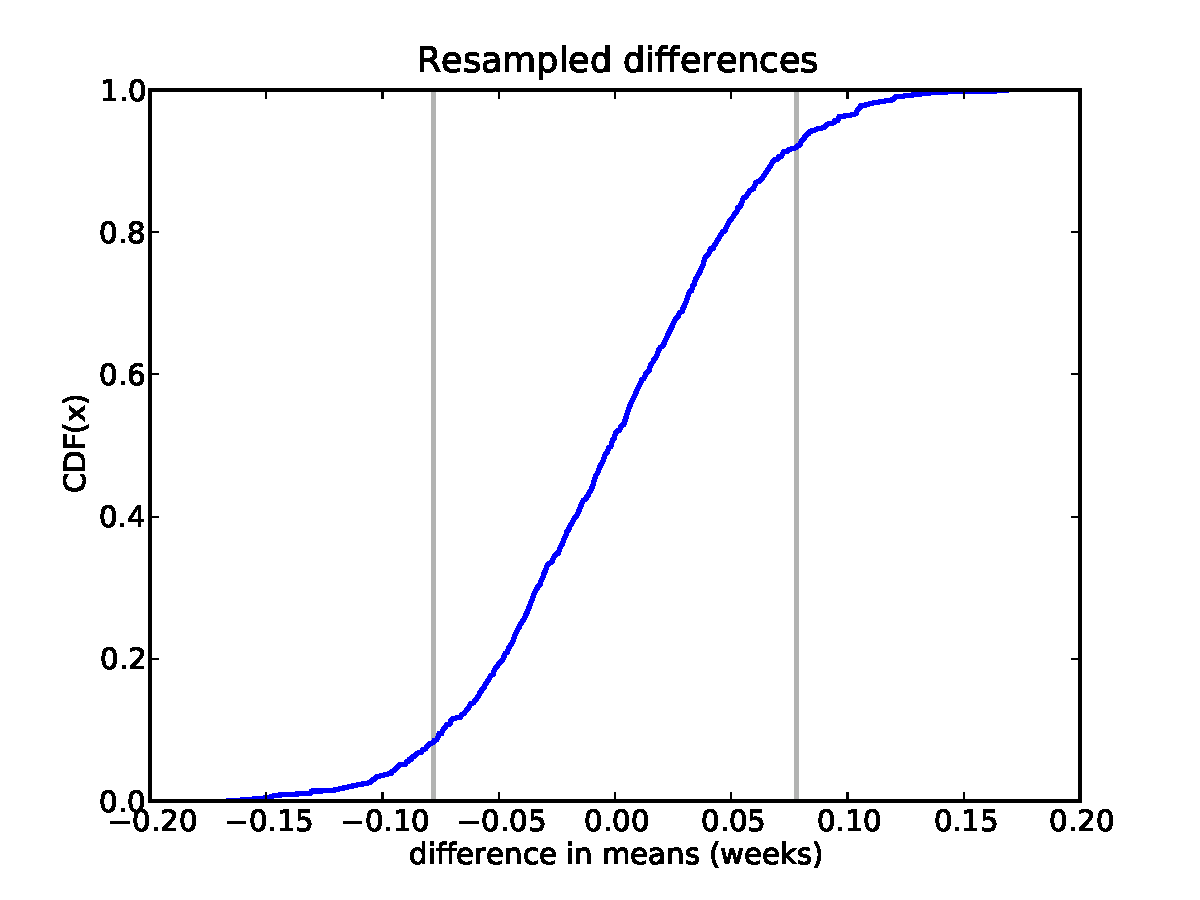
\includegraphics[height=2.5in]{figs/length_deltas_cdf.pdf}}
\caption{CDF of difference in mean for resampled data.}
\label{length_deltas_cdf}
\end{figure}

The mean difference is near 0, as you would expect with samples
from the same distribution.  The vertical lines show the cutoffs where
$x = -\delta$ or $x = \delta$.

Of 1000 sample pairs, there were 166 where the difference in means
(positive or negative) was as big or bigger than $\delta$, so the
p-value is approximately 0.166.  In other words, we expect to see an
effect as big as $\delta$ about 17\% of the time, even if the actual
distribution for the two groups is the same.

So the apparent effect is not very likely, but is it unlikely enough?
I'll address that in the next section.

\begin{exercise}
In the NSFG dataset, the difference in mean weight for first
births is 2.0 ounces.  Compute the p-value of this difference.
\index{National Survey of Family Growth}
\index{NSFG}

Hint: for this kind of resampling it is important to sample
with replacement, so you should use {\tt random.choice} rather
than {\tt random.sample} (see Section~\ref{random}).
\index{resampling}
\index{random module}

You can start with the code I used to generate the results in this
section, which you can download from \url{http://thinkstats2.com/hypothesis.py}.
\index{{\tt hypothesis.py}}

\end{exercise}


\section{Choosing a threshold}
\label{threshold}
\index{threshold}

In hypothesis testing we have to worry about two kinds of errors.
\index{false positive}
\index{false negative}
\index{error, Type I}
\index{error, Type II}

\begin{itemize}

\item A Type I error, also called a {\bf false positive}, is when we
  accept a hypothesis that is actually false; that is, we consider an
  effect significant when it was actually due to chance.

\item A Type II error, also called a {\bf false negative}, is when we
  reject a hypothesis that is actually true; that is, we attribute an
  effect to chance when it was actually real.

\end{itemize}

The most common approach to hypothesis testing is to choose a
threshold\footnote{Also known as a ``Significance criterion.''},
$\alpha$, for the p-value and to accept as significant any effect with
a p-value less than $\alpha$.  A common choice for $\alpha$ is 5\%.
By this criterion, the apparent difference in pregnancy length for
first babies is not significant, but the difference in weight is.
\index{significance criterion}
\index{pregnancy length}
\index{length!pregnancy}

For this kind of hypothesis testing, we can compute the probability of
a false positive explicitly: it turns out to be $\alpha$.

To see why, think about the definition of false positive---the chance
of accepting a hypothesis that is false---and the definition of a
p-value---the chance of generating the measured effect if the
hypothesis is false.

Putting these together, we can ask: if the hypothesis is false,
what is the chance of generating a measured effect that will be
considered significant with threshold $\alpha$?  The answer is
$\alpha$.

We can decrease the chance of a false positive by decreasing the
threshold.  For example, if the threshold is 1\%, there is only a 1\%
chance of a false positive.

But there is a price to pay: decreasing the threshold raises the
standard of evidence, which increases the chance of rejecting
a valid hypothesis.

In general there is a tradeoff between Type I and Type II errors.
The only way to decrease both at the same time is to increase the
sample size (or, if possible, decrease measurement error).
\index{sample size}

\begin{exercise}
To investigate the effect of sample size on p-value, see what happens
if you discard half of the data from the NSFG.  Hint: use {\tt
  random.sample}.  What if you discard three-quarters of the data, and
so on?
\index{National Survey of Family Growth}
\index{NSFG}

What is the smallest sample size where the difference in mean birth
weight is still significant with $\alpha$ = 5\%?  How much
larger does the sample size have to be with $\alpha$ = 1\%?

You can start with the code I used to generate the results in this
section, which you can download from
\url{http://thinkstats2.com/hypothesis.py}.  \index{{\tt
    hypothesis.py}}

\end{exercise}


\section{Defining the effect}

When something unusual happens, people often say something like,
``Wow!  What were the chances of {\em that}?''  This question makes
sense because we have an intuitive sense that some things are more
likely than others.  But this intuition doesn't always hold up to
scrutiny.
\index{chance}
\index{coin}

For example, suppose I toss a coin 10 times, and after each toss I
write down H for heads and T for tails.  If the result was a sequence
like THHTHTTTHH, you wouldn't be too surprised.  But if the result was
HHHHHHHHHH, you would say something like, ``Wow!  What were the
chances of {\em that}?''

But in this example, the probability of the two sequences is the
same: one in 1024.  And the same is true for any other sequence.
So when we ask, ``What were the chances of {\em that},'' we have
to be careful about what we mean by ``that.''

For the NSFG data, I defined the effect as ``a difference in mean
(positive or negative) as big or bigger than $\delta$.''  By making
this choice, I decided to evaluate the magnitude of the difference,
ignoring the sign.
\index{National Survey of Family Growth}
\index{NSFG}

A test like that is called {\bf two-sided}, because we consider both
sides (positive and negative) of the distribution shown in
Figure~\ref{length_deltas_cdf}.  By using a two-sided test we are
testing the hypothesis that there is a significant difference between
the distributions, without specifying the sign of the difference.
\index{one-sided test}
\index{two-sided test}
\index{test!one-sided}
\index{test!two-sided}

The alternative is to use a {\bf one-sided} test, which asks whether
the mean for first babies is significantly {\em higher} than
the mean for others.  Because the hypothesis is more specific, the
p-value is lower---in this case it is roughly half.


\section{Interpreting the result}

At the beginning of this chapter I said that the question we want to
address is whether an apparent effect is real.  We started by defining
the null hypothesis, denoted $H_{0}$, which is the hypothesis that
the effect is not real.  Then we defined the p-value, which is
$\Prob(E|H_{0})$, where $E$ is an effect as big as or bigger
than the apparent effect.  Then we computed p-values and compared them
to a threshold, $\alpha$.

That's a useful step, but it doesn't answer the original question,
which is whether the effect is real.  There are several ways to
interpret the result of a hypothesis test:

\begin{itemize}

\item Classical: In classical hypothesis testing, if a p-value
  is less than $\alpha$, you can say that the effect is statistically
  significant, but you can't conclude that it's real.  This
  formulation is careful to avoid leaping to conclusions, but it is
  unsatisfying because it provides no guidance for practical
  decision making.

\item Practical: In practice, people are not so formal.  In most
  science journals, researchers report p-values without apology, and
  readers interpret them as evidence that the apparent effect is real.
  The lower the p-value, the higher their confidence in this
  conclusion.

\end{itemize}


\section{Testing a correlation}

The NSFG data we saw in Section~\ref{} includes records for
xx preganancies.  For each pregnancy, we have the mother's age
and the baby's weight at birth, and we might wonder whether they
are correlated.  Do older mothers have heavier babies?  The
code I used to answer this question is available from
\url{}.

\begin{figure}
% correlate1.py
\centerline{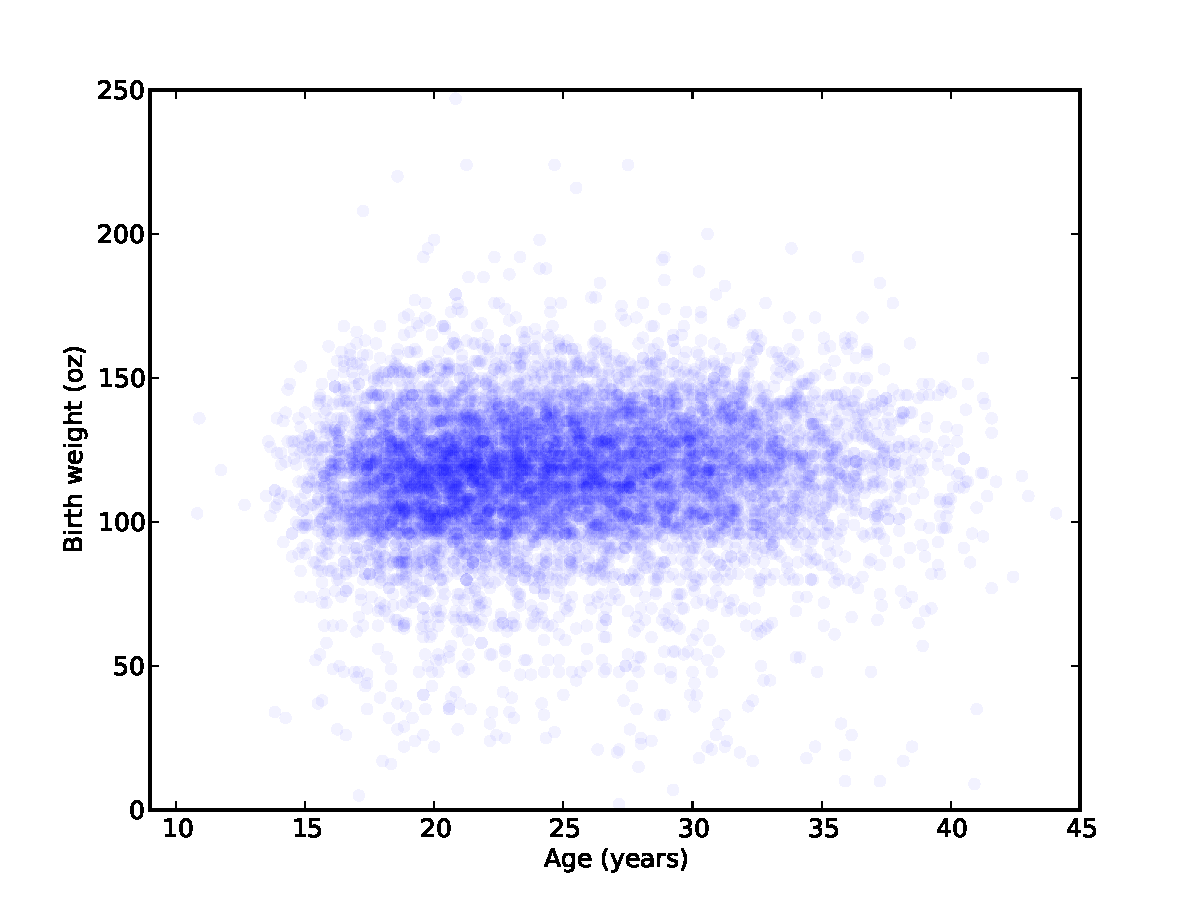
\includegraphics[height=2.5in]{figs/correlate1.pdf}}
\caption{Scatterplot of birth weight and mother's age for 13593 live
births.}
\label{correlate1}
\end{figure}

Here's the code that reads the data and extracts the relevant
variables:

\begin{verbatim}
def ReadData(data_dir='.'):
    preg = survey.Pregnancies()
    preg.ReadRecords(data_dir)
    print 'Number of pregnancies', len(preg.records)

    res = []
    for p in preg.records:
        if p.outcome == 1 and p.totalwgt_oz != 'NA':
            res.append((p.agepreg, p.totalwgt_oz))
    
    return zip(*res)
\end{verbatim}

And here's the code that makes a scatterplot of the data:

\begin{verbatim}
    xs, ys = ReadData(data_dir)

    thinkplot.Scatter(xs, ys, alpha=0.05)
    thinkplot.Show(xlabel='Age (years)',
                   ylabel='Birth weight (oz)')
\end{verbatim}

I chose {\tt alpha=0.05} to compromise between showing the densest
parts of the scatterplot without saturation and making the outliers
visible.  Figure~\ref{correlate1} shows the result.  Visually, it looks like
there might be a weak positive correlation, but it is hard to tell for sure.

For this dataset, Pearson's and Spearman's correlation coefficients
are 0.07 and 0.09.  Those numbers indicate weak correlations, so we
should wonder whether they might be due to chance.  As always, the question
we'll answer is, ``If there is no relationship between these variables,
what would be the chance of seeing a correlation as high as 0.07?''

There are several ways we could model the null hypothesis, but one of the
simplest is to shuffle the values of $x$ and $y$, like this:

\begin{verbatim}
def SimulateNull(xs, ys):
    random.shuffle(xs)
    random.shuffle(ys)
    return thinkstats2.Corr(xs, ys)
\end{verbatim}

This shuffle preserves the distribution of $x$ and $y$, but simulates
a hypothetical world where there is no relationship between them.
If we simulate this world 1000 times, we can see how often the null
hypothesis yields a correlation that exceeds what we actually saw:

\begin{verbatim}
def PValue(xs, ys, n=1000):
    actual = thinkstats2.Corr(xs, ys)

    xs_copy = list(xs)
    ys_copy = list(ys)

    corrs = []
    for i in range(n):
        corr = SimulateNull(xs_copy, ys_copy)
        corrs.append(corr)

    hits = [corr for corr in corrs if abs(corr) >= abs(actual)]
    p = len(hits) / float(n)
    return p
\end{verbatim}

{\tt actual} is the correlation between $x$ and $y$ before shuffling.
{\tt corrs} is the list of simulated correlations.  {\tt hits} is
the number of simulated correlations that exceed {\tt actual}.
And {\tt p} is the resulting p-value.

In this case, I compare the absolute value of {\tt corr} and {\tt
  actual}, so this is a two-sided test.  That's an appropriate choice
in this case because the hypothesis I am testing is whether there is
any relationship between these variables, positive or negative.  If I
suspected (before looking at the data) that there was a positive
relationship, I would use a one-sided test for that hypothesis.

The result in this case is 0, which means that after 1000 attempts,
the null hypothesis never yielded a correlation as high as 0.06.
The p-value is not actually 0.  If we keep trying, we will get a hit
eventually.  But the p-value is probably less than
1 in 1000, so I would report $p < 0.001$.

If we repeat the test with Spearman's correlation, the results are
similar.

This way of computing p-values is called a {\bf permutation test} because
when we shuffle {\tt xs} and {\tt ys} we get a permutation of the
original data.  Actually, shuffling either list is sufficient; shuffling
both doesn't make it any more random.


\section{Testing a linear regression}

With the same data from the previous section, we can use linear
least squares to estimate the slope and intercept of the relationship
between birth weight and mother's age.  Here's the code:

\begin{verbatim}
    xs, ys = ReadData(data_dir)
    inter, slope = thinkstats2.LeastSquares(xs, ys)
\end{verbatim}

The estimated value of {\tt inter} is 109 oz; the value of
{\tt slope} is 0.28 oz/year.  It is important to present estimates
like this in terms people can comprehend, so I would report
slope as 2.8 ounces per decade, or say, ``If the mother is
10 years older, we expect the baby to be 2.8 oz heavier.''

Interpreted literally, the intercept is the expected weight of
a baby if the mother is 0 years old.  Obviously, that doesn't
mean anything, so I would suggest reporting the value of the
fitted line for the mean or median age.  Here's the code that
computes the fitted line and prints the median birth weight
and age:

\begin{verbatim}
    fxs, fys = thinkstats2.FitLine(xs, inter, slope)
    i = len(fxs) / 2
    print 'median weight, age', fxs[i], fys[i]
\end{verbatim}

If the mother is 24, we expect the baby to weigh 116 oz (or 7.25 pounds).

Now that we have presented the results in human-comprehensible terms,
let's get back to hypothesis testing.  As always, we would like to
know whether the apparent relationship between these variables might
be due to chance.

One option is to use $R^2$ as a test statistic.  

\begin{verbatim}
    res = thinkstats2.Residuals(xs, ys, inter, slope)
    R2 = thinkstats2.CoefDetermination(ys, res)
\end{verbatim}

The result is $R^2 = 0.0047$.  So, the p-value we
want is the probability of seeing $R^2$ as big as that by chance.

As it happens, we have already computed this p-value.  Recall that
$R^2 = \rho^2$, so if $R^2$ exceeds 0.0047, the magnitude of $\rho$
must exceed $0.07$, which is the correlation we saw in the previous
section.  So a one-sided test of $R^2$ corresponds to a two-sided
test of $\rho$.  Based on the results of the previous section, we
conclude that the observed $R^2$ is statistically significant with
$p < 0.001$.

In addition, with linear regression we have the option of testing
each estimated parameter.  For example, we might like answer either
or both of these questions:

\begin{itemize}

\item If the actual intercept were 0, what would be the chance of
seeing an intercept as big as 109 oz?

\item If the actual slope were 0, what would be the chance of seeing
a slope as big as 0.28 oz/year?

\end{itemize}

The second question is often relevant in practice.  The first question
is not always relevant, unless we there is a theoretical reason to
expect the intercept to be 0.

To answer these questions, we model a null hypothesis
and compute the probability that the estimated parameter exceeds
the observed parameter under the null hypothesis.  For example,
if we are testing whether the slope is significant, the null hypothesis
is that the slope is actually 0.

If the slope is 0, the line that minimizes squared error is
$y = \ybar$; in this example, $\ybar$ is the mean birth weight.
Here's the code that computes the resulting residuals:

\begin{verbatim}
    xs, ys = ReadData(data_dir)
    inter = thinkstats2.Mean(ys)
    slope = 0
    fxs, fys = thinkstats2.FitLine(xs, inter, slope)
    res = thinkstats2.Residuals(xs, ys, inter, slope)
\end{verbatim}

Using the fitted line and the residuals, we can generate a simulation
of the null hypothesis by permutation:

\begin{verbatim}
def Permute(fxs, fys, res):
    random.shuffle(res)
    inter, slope = thinkstats2.LeastSquares(fxs, fys + res)
    return inter, slope
\end{verbatim}

{\tt Permute} takes the fitted values, {\tt fxs} and {\tt fys} and the
residuals, {\tt res}.  It shuffles the residuals, adds the shuffled
residuals to the fitted {\tt fys} and then computes a least squares
fit to the resulting simulated data.

\begin{figure}
% regress1.py
\centerline{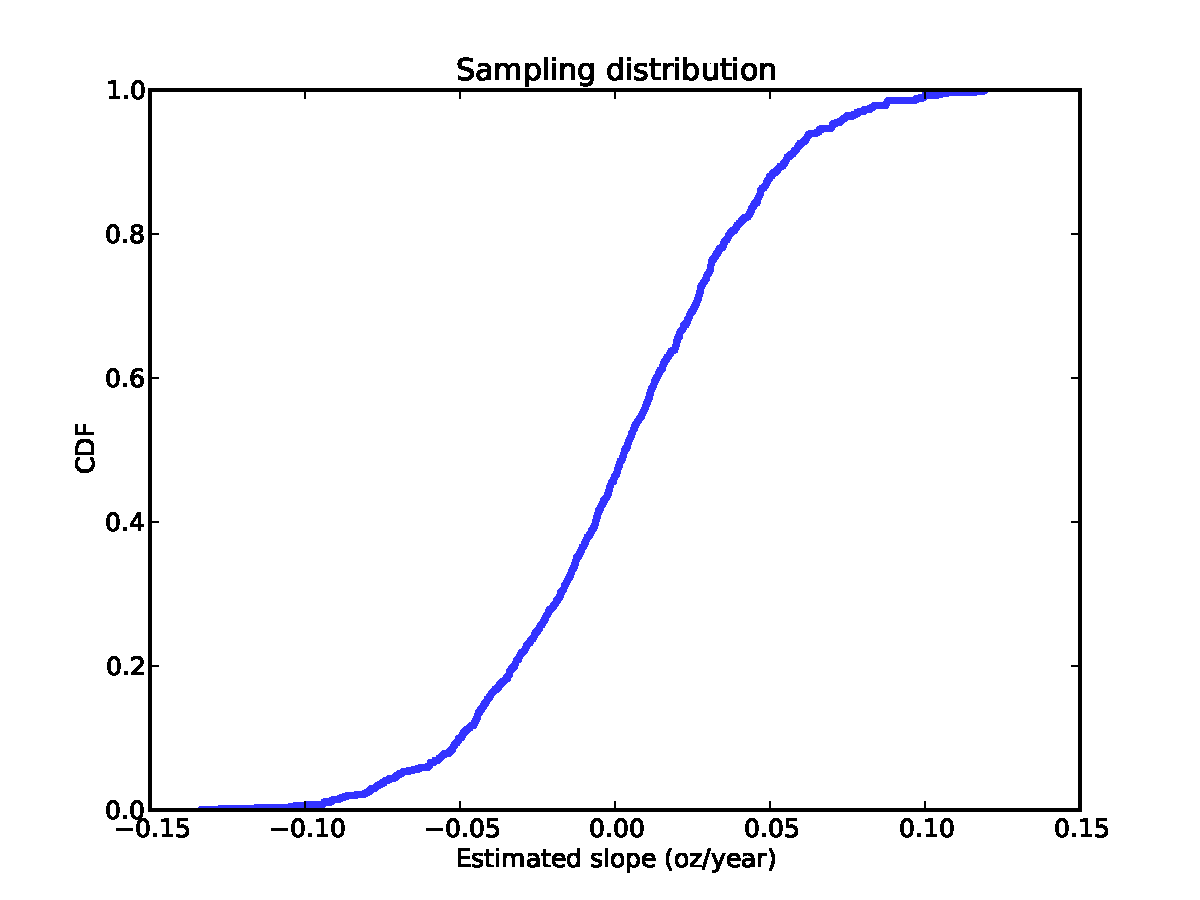
\includegraphics[height=2.5in]{figs/regress1.pdf}}
\caption{Sampling distribution of the estimated slope.}
\label{regress1}
\end{figure}

Each time we call {\tt Permute}, we get the result of another simulated
experiment.  If we call it 1000 times, we can estimate the sampling
distribution of {\tt slope} and {\tt intercept} under the null
hypothesis:

\begin{verbatim}
def SamplingDistributions(fxs, fys, res, n=10):
    res_copy = list(res)

    t = []
    for i in range(n):
        estimates = Permute(fxs, fys, res)
        t.append(estimates)

    inters, slopes = zip(*t)
    inter_cdf = thinkstats2.MakeCdfFromList(inters)
    slope_cdf = thinkstats2.MakeCdfFromList(slopes)

    return inter_cdf, slope_cdf
\end{verbatim}

{\tt SamplingDistributions} takes the fitted values, {\tt fxs} and {\tt fys},
the residuals, {\tt res}, and the number of iterations, {\tt n}.
It runs {\tt Permute} {\tt n} times and returns the accumulated
sampling distributions of {\tt inter} and {\tt slope}.

Figure~\ref{regress1} shows the sampling CDF of {\tt slope}.  The
upper bound, after 1000 tries, is about 0.12 oz/year.  So the
probability of seeing an estimated slope that exceeds the observed
value, 0.28 oz/year, is less than 1 in 1000.  We conclude that the
slope is statistically significant with $p < 0.001$.

To test the intercept, we find the line with {\tt inter=0} that
minimizes MSE, and use permutation to estimate the sampling
distribution of {\tt inter}.  In this example, the intercept is also
statistically significant with $p < 0.001$.


\section{Testing proportions}
\index{Chi-square test}

In Section~\ref{threshold} we concluded that the apparent difference
in mean pregnancy length for first babies and others was not
significant.  But in Section~\ref{relative.risk}, when we computed
relative risk, we saw that first babies are more likely to be early,
less likely to be on time, and more likely to be late.
\index{relative risk}
\index{pregnancy length}
\index{length!pregnancy}

So maybe the distributions have the same mean and different variance.
We could test the significance of the difference in variance, but
variances are less robust than means, and hypothesis tests for
variance often behave badly.
\index{mean}
\index{variance}
\index{hypothesis}

An alternative is to test a hypothesis that more directly reflects the
effect as it appears; that is, the hypothesis that first babies are
more likely to be early, less likely to be on time, and more likely to
be late.

We proceed in five easy steps:

\begin{enumerate}

\item We define a set of categories, called {\bf cells}, that each
  baby might fall into.  In this example, there are six cells because
  there are two groups (first babies and others) and three bins
  (early, on time or late).
\index{cell}

I'll use the definitions from Section~\ref{relative.risk}: a baby is
early if it is born during Week 37 or earlier, on time if it is born
during Week 38, 39 or 40, and late if it is born during Week 41 or
later.

\item We compute the number of babies we expect in each cell.  Under
  the null hypothesis, we assume that the distributions are the same
  for the two groups, so we can compute the pooled probabilities:
  $\Prob(early)$, $\Prob(ontime)$ and $\Prob(late)$.

For first babies, we have $n = 4413$ samples, so under the null
hypothesis we expect $n \cdot \Prob(early)$ first babies to be early,
$n \cdot \Prob(ontime)$ to be on time, etc.  Likewise, we have $m = 4735$
other babies, so we expect $m \cdot \Prob(early)$ other babies to be
early, etc.

\item For each cell we compute the deviation; that is, the difference
  between the observed value, $O_i$, and the expected value, $E_i$.
\index{test statistic}
\index{chi-square statistic}

\item We compute some measure of the total deviation; this quantity
is called the {\bf test statistic}.  The most common
choice is the chi-square statistic:
%
\[ \goodchi^2 = \sum_i \frac{(O_i - E_i)^2}{E_i} \]
%
%% Consider using upper case chi, which is more strictly correct,
%% but harder to distinguish from X.

\item We can use a Monte Carlo simulation to compute the p-value,
  which is the probability of seeing a chi-square statistic as high
  as the observed value under the null hypothesis.
\index{simulation!Monte Carlo}
\index{Monte Carlo}

\end{enumerate}

When the chi-square statistic is used, this process is called a 
{\bf chi-square test}.  One feature of the chi-square test is that
the distribution of the test statistic can be computed analytically.
\index{chi-square test}
\index{analysis}

Using the data from the NSFG I computed $\goodchi^{2} = 91.64$, which would
occur by chance about one time in 10,000.  I conclude that this result
is statistically significant, with one caution: we used the
same dataset for exploration and testing.  It would be a good idea
to confirm this result with another dataset.
\index{National Survey of Family Growth}
\index{NSFG}

You can download the code I used in this section from
\url{http://thinkstats2.com/chi.py}.
\index{{\tt chi.py}}

% See \url{http://en.wiktionary.org/wiki/voila}!


\begin{exercise}
Suppose you run a casino and you suspect that a customer has
replaced a die provided by the casino with a ``crooked die;'' that
is, one that has been tampered with to make one of the faces more
likely to come up than the others.  You apprehend the alleged
cheater and confiscate the die, but now you have to prove that it
is crooked.
\index{casino}
\index{dice}
\index{crooked die}

You roll the die 60 times and get the following results:

\begin{center}
\begin{tabular}{|l|c|c|c|c|c|c|}
\hline
Value     &  1  &  2  &  3  &  4  &  5  &  6  \\ 
\hline
\hline
Frequency &  8  &  9  &  19  &  6  &  8  &  10  \\
\hline
\end{tabular}
\end{center}

What is the chi-squared statistic for these values?  What is the
probability of seeing a chi-squared value as large by chance?

\end{exercise}


\section{Power}
\index{power}

When the result of a hypothesis test is negative (that is, the effect is
not statistically significant), can we conclude that the effect is not
real?  That depends on the power of the test.

Statistical {\bf power} is the probability that the test will be
positive if the null hypothesis is false.  In general, the power of a
test depends on the sample size, the magnitude of the effect, and the
threshold $\alpha$.

% TODO: replace this with the calculation

\begin{exercise}
What is the power of the test in Section~\ref{threshold}, using
$\alpha$ = 0.05 and assuming that the actual difference between the
means is 0.078 weeks?

You can estimate power by generating random samples from distributions
with the given difference in the mean, testing the observed difference
in the mean, and counting the number of positive tests.

What is the power of the test with $\alpha$ = 0.10?

\end{exercise}

One way to report the power of a test, along with a negative result,
is to say something like, ``If the apparent effect were as large
as $x$, this test would reject the null hypothesis with probability $p$.''


%\section{Discussion}

%Pitfalls:

%1) Exploring and then testing

%2) Multiple tests

%3) Publication bias


%Solutions:

%1) two phases: exploratory and testing, on different data (possibly a subset)

%2) Holm-Bonferroni method

%3) publish everything and wait for consensus


\section{Glossary}

\begin{itemize}

\item significant: An effect is statistically significant if it is unlikely
to occur by chance.
\index{significant}

\item null hypothesis: A model of a system based on the assumption that
an apparent effect is due to chance.
\index{null hypothesis}

\item p-value: The probability that an effect could occur by chance.
\index{p-value}

\item hypothesis testing: The process of determining whether an apparent
effect is statistically significant.
\index{hypothesis testing}

\item permutation test: A way to compute p-values by generating
  permutations of an observed dataset.
  \index{permutation test}

\item false positive: The conclusion that an effect is real when it is not.
\index{false positive}

\item false negative: The conclusion that an effect is due to chance when it
is not.
\index{false negative}

\item two-sided test: A test that asks, ``What is the chance of an effect
as big as the observed effect, positive or negative?''

\item one-sided test: A test that asks, ``What is the chance of an effect
as big as the observed effect, and with the same sign?''
\index{one-sided test}
\index{two-sided test}
\index{test!one-sided}
\index{test!two-sided}

\item test statistic: A statistic used to measure the deviation of an
apparent effect from what is expected by chance.
\index{test statistic}

\item chi-square test: A test that uses the chi-square statistic as
the test statistic.
\index{ch-square test}

\item cell: In a chi-square test, the categories the observations are
divided into.
\index{cell}

\item power: The probability that a test will reject the null hypothesis
if it is false.
\index{power}

\end{itemize}



\chapter{Multiple regression}

\section{Weighted resampling}


\chapter{Logistic regression}


\chapter{Time series analysis}



\chapter{Survival analysis}


\chapter{Analytic statistics}

\section{Estimation}

\section{Hypothesis testing}


\printindex

\clearemptydoublepage
%\blankpage
%\blankpage
%\blankpage


\end{document}

%Chapter 10: time series

%serial correlation

%auto-correlation function

%generating random series with correlation

%violating the CLT and see if the sum of correlated normals is lognormal

%If so, maybe that explains adult weight distribution.




% Topics to consider in the future:

% Time series

% Correlation of adjacent elements

% Autocorrelation function

% Information theory: Paul Revere example

% Gelman's paradox
% \url{http://www.iq.harvard.edu/blog/sss/archives/2008/04/gelmans_paradox.shtml}

% regression to the mean experiment

% Poisson distribution

% example using csvDictReader


\section{Conditional probability}
\index{conditional probability}
\index{probability!conditional}

Imagine that someone you know is pregnant, and it is the beginning of
Week 39.  What is the chance that the baby will be born in the next
week?  How much does the answer change if it's a first baby?

We can answer these questions by computing a {\bf conditional
probability}, which is (ahem!) a probability that depends on a condition.
In this case, the condition is that we know the baby didn't arrive
during Weeks 0--38.

Here's one way to do it:

\begin{enumerate}

\item Given a PMF, generate a fake cohort of 1000 pregnancies.
For each number of weeks, x, the number of pregnancies with
duration x~is 1000 PMF(x).
\index{cohort}

\item Remove from the cohort all pregnancies with length less than 39.
\index{pregnancy length}
\index{length!pregnancy}

\item Compute the PMF of the remaining durations; the result is the
conditional PMF.

\item Evaluate the conditional PMF at $x = 39$ weeks.

\end{enumerate}

This algorithm is conceptually clear, but not very efficient.
A simple alternative is to remove from the distribution the values
less than 39 and then renormalize.

\begin{exercise}
Write a function that implements either of these algorithms and
computes the probability that a baby will be born during Week 39,
given that it was not born prior to Week 39.

Generalize the function to compute the
probability that a baby will be born during Week x, given that
it was not born prior to Week x, for all x.
Plot this value as a function of x~for first babies and others.

You can download a solution to this problem from
\url{http://thinkstats2.com/conditional.py}.
\index{{\tt conditional.py}}

\end{exercise}


\chapter{Probability}

\newcommand{\Poincare}{Poincar\'{e}}

\section{\Poincare}
%\index{\Poincare, Henry}

Henri \Poincare~was a French mathematician who taught at the Sorbonne
around 1900.  The following anecdote about him is probably fabricated,
but it makes an interesting probability problem.
\index{bread police}

Supposedly \Poincare~suspected that his local bakery was selling
loaves of bread that were lighter than the advertised weight of 1 kg,
so every day for a year he bought a loaf of bread, brought it home and
weighed it.  At the end of the year, he plotted the distribution of
his measurements and showed that it fit a normal distribution with
mean 950 g and standard deviation 50 g.  He brought this evidence to
the bread police, who gave the baker a warning.
\index{normal distribution}
\index{distribution!normal}
\index{Gaussian distribution}
\index{distribution!Gaussian}

For the next year, \Poincare~continued the practice of weighing his
bread every day.  At the end of the year, he found that the average
weight was 1000 g, just as it should be, but again he complained to
the bread police, and this time they fined the baker.
\index{symmetric}

Why?  Because the shape of the distribution was asymmetric.  Unlike
the normal distribution, it was skewed to the right, which is
consistent with the hypothesis that the baker was still making 950 g
loaves, but deliberately giving \Poincare~the heavier ones.


\begin{exercise}
Write a program that simulates a baker who chooses $n$ loaves from a
distribution with mean 950 g and standard deviation 50 g, and gives
the heaviest one to \Poincare.  What value of $n$ yields a
distribution with mean 1000 g?  What is the standard deviation?

Compare this distribution to a normal distribution with the same mean
and the same standard deviation.  Is the difference in the shape of
the distribution big enough to convince the bread police?

\end{exercise}


\begin{exercise}
\label{coef_var}
If you go to a dance where partners are paired up randomly, what
percentage of opposite sex couples will you see where the woman is
taller than the man?
\index{dance}
\index{height}
\index{Behavioral Risk Factor Surveillance System}
\index{BRFSS}

In the BRFSS (see Section~\ref{lognormal}), the distribution of
heights is roughly normal with parameters $\mu$ = 178 cm and
$\sigma^2 = 59.4$ cm for men, and $\mu$ = 163 cm and $\sigma^2 = 52.8$ cm for
women.
\index{lognormal distribution}
\index{distribution!lognormal}

\end{exercise}


\section{Streaks and hot spots}
\index{streak}
\index{hot spot}
\index{random}

People do not have very good intuition for random processes.  If you
ask people to generate ``random'' numbers, they tend to generate
sequences that are random-looking, but actually more ordered than real
random sequences.  Conversely, if you show them a real random
sequence, they tend to see patterns where there are none.

An example of the second phenomenon is that many people believe
in ``streaks'' in sports: a player that has been successful recently
is said to have a ``hot hand;'' a player that has been unsuccessful is
``in a slump.''
\index{hot hand}
\index{slump}
\index{sport}

Statisticians have tested these hypotheses in a number of sports, and
the consistent result is that there is no such thing as a
streak\footnote{For example, see Gilovich, Vallone and Tversky, ``The
  hot hand in basketball: On the misperception of random sequences,''
  1985.}.  If you assume that each attempt is independent of previous
attempts, you will see occasional long strings of successes or
failures.  These apparent streaks are not sufficient evidence that
there is any relationship between successive attempts.
\index{clustering illusion}
\index{spatial pattern}

A related phenomenon is the clustering illusion, which is the
tendency to see clusters in spatial patterns that are actually
random (see \url{http://wikipedia.org/wiki/Clustering_illusion}).
\index{simulation!Monte Carlo}
\index{Monte Carlo}

To test whether an apparent
cluster is likely to be meaningful, we can simulate the behavior
of a random system to see whether it is likely to produce a similar
cluster.  This process is called {\bf Monte Carlo} simulation because
generating random numbers is reminiscent of casino games (and Monte
Carlo is famous for its casino).

\begin{exercise}
If there are 10 players in a basketball game and each one takes
15 shots during the course of the game, and each shot has a
50\% probability of going in, what is the probability that 
you will see, in a given game, at least one player who
hits 10 shots in a row?  If you watch a season of 82 games,
what are the chances you will see at least one streak of
10 hits or misses?
\index{basketball}
\index{simulation!Monte Carlo}
\index{Monte Carlo}

This problem demonstrates some strengths and weaknesses of Monte
Carlo simulation.  A strength is that it is often easy and fast
to write a simulation, and no great knowledge of probability is
required.  A weakness is that estimating the probability of
rare events can take a long time!  A little bit of analysis can
save a lot of computing.

\end{exercise}


\begin{exercise}
In 1941 Joe DiMaggio got at least one hit
in 56 consecutive games\footnote{See
  \url{http://wikipedia.org/wiki/Hitting_streak}.}.  Many baseball fans
consider this streak the greatest achievement in any sport in history,
because it was so unlikely.
\index{baseball}
\index{DiMaggio, Joe}
\index{hitting streak}
\index{simulation!Monte Carlo}
\index{Monte Carlo}

Use a Monte Carlo simulation to estimate the probability that
any player in major league baseball will have a hitting streak
of 57 or more games in the next century.

\end{exercise}


\begin{exercise}
A cancer cluster is defined by the Centers for Disease Control (CDC)
as ``greater-than-expected number of cancer cases that occurs within a
group of people in a geographic area over a period of
time.\footnote{From \url{http://cdc.gov/nceh/clusters/about.htm}.}''
\index{cluster}
\index{cancer cluster}
\index{Gawande, Atul}

Many people interpret a cancer cluster as evidence of an environmental
hazard, but many scientists and statisticians think that investigating
cancer clusters is a waste of time\footnote{See Gawande, ``The Cancer
  Cluster Myth,'' {\em New Yorker}, Feb 8, 1997.}.  Why?  One reason
(among several) is that identifying cancer clusters is a classic case
of the Sharpshooter Fallacy (see
\url{http://wikipedia.org/wiki/Texas_sharpshooter_fallacy}).
\index{sharpshooter fallacy}
\index{fallacy!sharpshooter}

Nevertheless, when someone reports a cancer cluster, the CDC is
obligated to investigate.  According to their web page:

\begin{quote}

``Investigators develop a `case' definition, a time period of concern,
  and the population at risk. They then calculate the expected number
  of cases and compare them to the observed number. A cluster is
  confirmed when the observed/expected ratio is greater than 1.0, and
  the difference is statistically significant.''

\end{quote}

\begin{enumerate}

\item Suppose that a particular cancer has an incidence of 1 case per
  thousand people per year.  If you follow a particular cohort of 100
  people for 10 years, you would expect to see about 1 case.  If you
  saw two cases, that would not be very surprising, but more than than
  two would be rare.\index{cohort}

  Write a program that simulates a large number of cohorts over
  a 10 year period and estimates the distribution of total cases.

\item An observation is considered statistically significant if its
  probability by chance alone, called a p-value, is less than 5\%.
  In a cohort of 100 people over 10 years, how many cases would you
  have to see to meet this criterion?

\item Now imagine that you divide a population of 10000 people into 100
  cohorts and follow them for 10 years.  What is the chance that at
  least one of the cohorts will have a ``statistically significant''
  cluster?  What if we require a p-value of 1\%?

\item Now imagine that you arrange 10000 people in a $100 \times 100$
  grid and follow them for 10 years.  What is the chance that there
  will be at least one $10 \times 10$ block anywhere in the grid
  with a statistically significant cluster?

\item Finally, imagine that you follow a grid of 10000 people for 30
  years.  What is the chance that there will be a 10-year interval
  at some point with a $10 \times 10$ block anywhere in the grid
  with a statistically significant cluster?

\end{enumerate}

\end{exercise}




\section{Efficient resampling}
\index{resampling}

Anyone reading this book who has prior training in statistics probably
laughed when they saw Figure~\ref{length_deltas_cdf}, because I used a
lot of computer power to simulate something I could have figured out
analytically.
\index{analysis}
\index{pregnancy length}
\index{length!pregnancy}

Obviously mathematical analysis is not the focus of this book.  I am
willing to use computers to do things the ``dumb'' way, because I
think it is easier for beginners to understand simulations, and easier
to demonstrate that they are correct.  So as long as the simulations
don't take too long to run, I don't feel guilty for skipping the
analysis.

However, there are times when a little analysis can save a lot of
computing, and Figure~\ref{length_deltas_cdf} is one of those times.
\index{mean, difference in}

Remember that we were testing the observed difference in the mean between
pregnancy lengths for $n = 4413$ first babies and $m = 4735$ others.  We formed
the pooled distribution for all babies, drew samples with sizes $n$ and
$m$, and computed the difference in sample means.
\index{sample mean}

Instead, we could directly compute the distribution of the difference
in sample means.  To get started, let's think about what a sample mean
is: we draw $n$ samples from a distribution, add them up, and
divide by n.  If the distribution has mean $\mu$ and variance
$\sigma^2$, then by the Central Limit Theorem, we know that the sum of
the samples is $\normal (n \mu, n \sigma^2)$.
\index{normal distribution}
\index{distribution!normal}
\index{Gaussian distribution}
\index{distribution!Gaussian}

To figure out the distribution of the sample means, we have to invoke
one of the properties of the normal distribution: if X~is
$\normal (\mu, \sigma^2)$,

\[ aX~+~b~\sim~\normal(a \mu~+~b, a^{2} \sigma^2)\]

When we divide by n, $a = 1/n$ and $b = 0$, so
%
\[ X/n~\sim~\normal(\mu /n, \sigma^2/ n^{2}) \]
%
So the distribution of the sample mean is $\normal (\mu, \sigma^2/n)$.

To get the distribution of the difference between two sample means,
we invoke another property of the normal distribution: if $X_{1}$ is
$\normal (\mu_{1}, \sigma_{1}^{2})$ and $X_{2}$ is
$\normal (\mu_{2}, \sigma_{2}^{2})$,
%
\[ aX_1 + bX_2 \sim \normal(a\mu_1 + b\mu_2, 
                                 a^2\sigma_1^2 + b^2\sigma_2^2) \]
%
So as a special case:
%
\[ X_1 - X_2 \sim \normal(\mu_1 - \mu_2, 
                               \sigma_1^2 + \sigma_2^2) \]
%
Putting it all together, we conclude that the sample in
Figure~\ref{length_deltas_cdf} is drawn from 
$\normal (0, f \sigma^2)$, where $f = 1/n~+~1/m$.  Plugging in
n = 4413 and m = 4735, we expect the difference of sample means to be
$\normal (0, 0.0032)$.
\index{p-value}

We can use {\tt erf.NormalCdf} to compute the p-value of the observed 
difference in the means:
%
\begin{verbatim}
delta = 0.078
sigma = math.sqrt(0.0032)
left = erf.NormalCdf(-delta, 0.0, sigma)
right = 1 - erf.NormalCdf(delta, 0.0, sigma)
\end{verbatim}

The sum of the left and right tails is the p-value, 0.168, which is
pretty close to what we estimated by resampling, 0.166. 
You can download the code I used in this section from
\url{http://thinkstats2.com/hypothesis_analytic.py}
\index{{\tt hypothesis\_analytic.py}}

\section{Significance}

In the previous exercise, you compared the gestation period for first
babies and others; if things worked out, you found that first
babies are born about 13 hours later, on average.
\index{apparent effect}

A difference like that is called an {\bf apparent effect}; that is,
there might be something going on, but we are not yet sure.  There are
several questions we still want to ask:

\begin{itemize}

\item If the two groups have different means, what about other {\bf
  summary statistics}, like median and variance?  Can we be more
  precise about how the groups differ?
\index{summary statistic}

\item Is it possible that the difference we saw could occur by chance,
  even if the groups we compared were actually the same?  If so,
  we would conclude that the effect was not {\bf statistically
    significant}.
\index{statistically significant}
\index{significance}


\item Is it possible that the apparent effect is due to selection bias or
  some other error in the experimental setup?  If so, then we might
  conclude that the effect is an {\bf artifact}; that is, something we
  created (by accident) rather than found. 
\index{artifact}

\end{itemize}

Answering these questions will take most of the rest of this book.

